%%%%%%%%%%%%%%%%%%%%%%%%%%%%%%%%%%%%%%%%%%%%%%%%%%%%%%%%%%%%%%%%%%%%%%%%%%%%%%%%
%%%%%%%%%%%%%%%%%%   Vorlage für eine Abschlussarbeit   %%%%%%%%%%%%%%%%%%%%%%%%
%%%%%%%%%%%%%%%%%%%%%%%%%%%%%%%%%%%%%%%%%%%%%%%%%%%%%%%%%%%%%%%%%%%%%%%%%%%%%%%%

% Erstellt von Maximilian Nöthe, <maximilian.noethe@tu-dortmund.de>
% ausgelegt für lualatex und Biblatex mit biber

% Kompilieren mit
% latexmk --lualatex --output-directory=build thesis.tex
% oder einfach mit:
% make

\documentclass[
  tucolor,       % remove for less green,
  BCOR=12mm,     % 12mm binding corrections, adjust to fit your binding
  parskip=half,  % new paragraphs start with half line vertical space
  open=any,      % chapters start on both odd and even pages
  cleardoublepage=plain,  % no header/footer on blank pages
]{tudothesis}


% Warning, if another latex run is needed
\usepackage[aux]{rerunfilecheck}

% just list chapters and sections in the toc, not subsections or smaller
\setcounter{tocdepth}{1}

%------------------------------------------------------------------------------
%------------------------------ Fonts, Unicode, Language ----------------------
%------------------------------------------------------------------------------
\usepackage{fontspec}
\defaultfontfeatures{Ligatures=TeX}  % -- becomes en-dash etc.

% load english (for abstract) and ngerman language
% the main language has to come last
\usepackage[american, ngerman]{babel}

% intelligent quotation marks, language and nesting sensitive
\usepackage[autostyle]{csquotes}

% microtypographical features, makes the text look nicer on the small scale
\usepackage{microtype}

%------------------------------------------------------------------------------
%------------------------ Math Packages and settings --------------------------
%------------------------------------------------------------------------------

\usepackage{amsmath}
\usepackage{amssymb}
\usepackage{mathtools}
\usepackage{listings} % allows to present code

% Enable Unicode-Math and follow the ISO-Standards for typesetting math
\usepackage[
  math-style=ISO,
  bold-style=ISO,
  sans-style=italic,
  nabla=upright,
  partial=upright,
  warnings-off={mathtools-colon,mathtools-overbracket}, % suppress some unnecessary warnings
]{unicode-math}
\setmathfont{Latin Modern Math}

% nice, small fracs for the text with \sfrac{}{}
\usepackage{xfrac}


%------------------------------------------------------------------------------
%---------------------------- Numbers and Units -------------------------------
%------------------------------------------------------------------------------

\usepackage[
  locale=DE,
  separate-uncertainty=true,
  per-mode=symbol-or-fraction,
]{siunitx}

%------------------------------------------------------------------------------
%-------------------------------- tables  -------------------------------------
%------------------------------------------------------------------------------

\usepackage{booktabs}       % \toprule, \midrule, \bottomrule, etc

%------------------------------------------------------------------------------
%-------------------------------- graphics -------------------------------------
%------------------------------------------------------------------------------

\usepackage{graphicx}
\usepackage{wrapfig}
% currently broken
% \usepackage{grffile}

% allow figures to be placed in the running text by default:
\usepackage{scrhack}
\usepackage{float}
\floatplacement{figure}{htbp}
\floatplacement{table}{htbp}

% keep figures and tables in the section
\usepackage[section, below]{placeins}

% allows to include PDFs as full pages
\usepackage{pdfpages}

% Set the PDF Version of this document to 1.7 (1.4 is the current default)
% This is needed so that PDFs with Version >1.5 can be included
\pdfvariable minorversion=7

%------------------------------------------------------------------------------
%---------------------- customize list environments ---------------------------
%------------------------------------------------------------------------------

\usepackage{enumitem}

%------------------------------------------------------------------------------
%------------------------------ Bibliographie ---------------------------------
%------------------------------------------------------------------------------

\usepackage[
  backend=biber,   % use modern biber backend
  autolang=hyphen, % load hyphenation rules for if language of bibentry is not
                   % german, has to be loaded with \setotherlanguages
                   % in the references.bib use langid={en} for english sources
]{biblatex}
\addbibresource{references.bib}  % the bib file to use
\DefineBibliographyStrings{german}{andothers = {{et\,al\adddot}}}  % replace u.a. with et al.


% Last packages, do not change order or insert new packages after these ones
\usepackage[pdfusetitle, unicode, linkbordercolor=tugreen, citebordercolor=tugreen]{hyperref}
\usepackage{bookmark}
\usepackage[shortcuts]{extdash}

%------------------------------------------------------------------------------
%-------------------------    Angaben zur Arbeit   ----------------------------
%------------------------------------------------------------------------------

\author{Samuel Haefs}
\title{\Huge Lösungen inverser Probleme}
\subtitle{\LARGE Entfaltung von Energiespektren mit \\ neuronalen Netzen in DSEA}
\date{2022}
\birthplace{Herdecke}
\chair{Lehrstuhl für Experimentelle Physik V}
\division{Fakultät Physik}
\thesisclass{Bachelor of Science}
\submissiondate{30. August 2022}
\firstcorrector{Prof.~Dr.~Dr.~Rhode}
\secondcorrector{Prof.~Dr.~Albrecht}

% tu logo on top of the titlepage
\titlehead{
\includegraphics[height=1.5cm]{logos/tu-logo.pdf}}

\begin{document}
\frontmatter
\maketitle

% Gutachterseite
\makecorrectorpage

% hier beginnt der Vorspann, nummeriert in römischen Zahlen
\thispagestyle{plain}

\section*{Kurzfassung}
Physiker und Physikerinnen werden ständig mit inversen Problemen konfrontiert.
%Auf Lösungen inverser Probleme ist zum Beispiel das Hochenergie-Neutrino-Observatorium \texit{IceCube} angewiesen.
Über die Zeit wurden verschiedene Methoden zur Lösung entwickelt.
Der \textbf{D}ortmund \textbf{S}pectrum \textbf{E}stimation \textbf{A}lgorithm (DSEA) fasst das zugrundeliegende Problem als Klassifikationsaufgabe auf.
Dabei können verschiedene Klassifikationsalgorithmen verwendet werden.
Der Einsatz von neuronalen Netzen als Klassifizierer in DSEA ist ein neuer Ansatz und wird auf IceCube-Neutrino Simulationen untersucht.
Neuronale Netze in DSEA bieten die Möglichkeit den Trainingsprozess weiter fortzuführen, statt einen Klassifizierer in jeder Iteration neu zuinitalisieren.
Systematisch werden die Hyperparameter des neuronalen Netzes und von DSEA untersucht.
Ein häufiges Problem neuronaler Netze ist die Überanpassung an die Trainingsdaten.
Es wird geprüft, ob die Modelle eine unabhängige Vorhersage treffen.

\section*{Abstract}
\begin{foreignlanguage}{english}
Physicists are frequently confronted with inverse problems.
Over time, various methods have been developed to solve them.
The \textbf{D}ortmund \textbf{S}pectrum \textbf{E}stimation \textbf{A}lgorithm (DSEA) treats the fundamental problem as a classification task.
Various classification algorithms can be used.
The use of neural networks as classifier in DSEA is a new approach and is explored on IceCube neutrino simulations.
Neural networks in DSEA offer the possibility to continue the training process, instead of reinitializing the classifier in each iteration.
Systematically, the hyperparameters of the neural network and DSEA are investigated.
A common problem of neural networks is overfitting to the training data.
The models are tested for unbiased predictions.
\end{foreignlanguage}

\tableofcontents

\mainmatter
% Hier beginnt der Inhalt mit Seite 1 in arabischen Ziffern
\chapter{Einleitung}
Die Astroteilchenphysik untersucht aller Art Teilchen, die von extraterrestrischen Quellen ausgesandt wurden.
Ziel ist die Bestimmung der Position und der Eigenschaften von Himmelskörpern über die ankommenden Botenteilchen.
Die Botenteilchen setzen sich aus geladenen Teilchen (kosmische Strahlung), Photonen $\gamma$ und Neutrinos $\nu$ zusammen.\cite{icecube_detector}
\\
\\
IceCube ist ein Detektor am geographischen Südpol und ist dafür ausgelegt, hochenergetische Neutrinos nachzuweisen.
Zum einen ist der Ort der Neutrinoquelle von großer Interesse.
Aktive Galaxiekerne, schwarze Löcher oder auch Neutronensterne können mögliche Quellen der Neutrinos sein und sind für Physiker*innen von großem Interesse.
Eine weitere wichtige Größe stellt das Energiespektrum der Neutrinos dar.
\\
Die Neutrinoenergie ist nicht direkt messbar.
Stattdessen werden die Zerfallsprodukte der Neutrinos (Elektronen, Myonen, Tau-Leptonen) gemessen.
Das zu lösende Problem ist die Rekonstruktion der Neutrinoenergie aus den gemessenen Größen.
Es handelt sich um ein inverses Problem, welches grundsätzlich schlecht konditioniert ist.
Die Rekonstruktion der Energie wird als Entfaltung bezeichnet und benötigt spezielle Ansätze.
\\
\\
Der \textbf{D}ortmund \textbf{S}pectrum \textbf{E}stimation \textbf{A}lgorithm (DSEA) \cite{ruhe} betrachtet das Problem als Klassifikationsproblem.
Unter Verwendung von Methoden des maschinellen Lernens kann eine Entfaltung mit DSEA durchgeführt werden.
\\
In dieser Arbeit wird zum ersten mal die Verwendung von neuronalen Netzen als Klassifizierer in DSEA untersucht.
Dies bietet neue Möglichkeiten.
Die bisher verwendeten Klassifizierer wurden in jeder DSEA-Iteration neu initialisiert.
Neuronale Netze basieren auf einer Verlustfunktion.
Es ist daher möglich den Trainingsprozess eines Modells fortzuführen, statt in jeder DSEA-Iteration von neuem zu beginnen.
\\
Die Struktur eines neuronalen Netzes kann an das zugrundeliegende Problem angepasst werden.
Es gibt eine große Auswahl an Ebenen, Verlustfunktionen und Aktivierungsfunktionen.
Duch Anpassung der Hyperparameter kann die Lösung optimiert werden.
\chapter{Physikalische Grundlagen}
In disem Kapitel wird der physikalische Hintergrund zu dieser Arbeit behandelt.
Zuerst wird auf den Aufbau des IceCube-Neutrino-Observatoriums eingegangen und dabei die Funktionsweise des Detektors erläutert.
Anschließend werden kurz wichtige Aspekte der Neutrinophysik aufgeführt.

% ICECUBE
\section{IceCube-Neutrino-Observatorium} \label{sec:icecube}

IceCube ist ein Hochenergie-Neutrino-Observatorium am geographischen Südpol.
Der Detektor befindet sich in einer Tiefe von \SIrange{1450}{2450}{\metre} im antarktischen Eis und deckt ein Volumen von \SI{1}{\kilo\metre^3} ab.\cite{icecube_detector}
An 86 Strings sind in regelmäßigen Abständen DOMs (Digital Optical Module) angebracht.
Der Detektoraufbau ist schematisch in der \autoref{fig:detector} dargestellt.
\begin{figure}
    \centering
    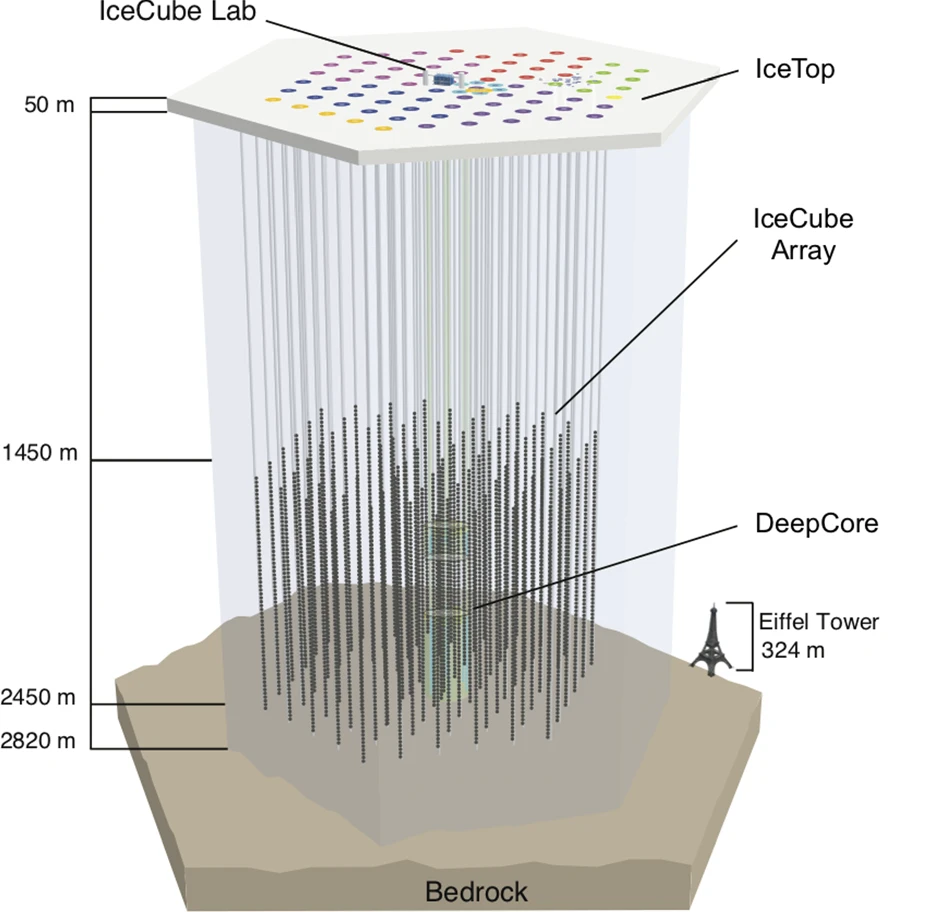
\includegraphics[width=0.5\textwidth]{Plots/detector2.png}
    \caption[IceCube-Detektor und IceTop Array]{Schematische Darstellung des sich im antarktischen Eis befindenden IceCube-Detektors und des IceTop Arrays.
    IceCube liegt \SIrange{1450}{2450}{\metre} unter dem Eis und beinhaltet den Teildetektor DeepCore.
    Jeder Punkt stellt einen DOM und jeder Kreis eine IceTop-Station auf der Eisoberfläche dar \cite{Ahlers_2018}.
    }
    \label{fig:detector}
\end{figure}

Ein großer Teil des DOMs besteht aus einem Photomultiplier der Licht im Wellenlängenbereich \SIrange{300}{650}{\nano\metre} registriert.
Hochenergetische Neutrinos wechselwirken mit dem Eis und zerfallen in Leptonen (Elektron, Myon, Tau-Lepton).
Aufgrund der Enegieerhaltung besitzen die Leptonen eine hohe kinetische Energie.
Sie bewegen sich mit einer Geschwindigkeit $v$ die größer als die Lichtgeschwindigkeit im Medium $c_m$ ist durch das Eis.
Dabei wird kegelförmig Cherenkov-Strahlung\cite{landau2013electrodynamics} im Winkel $\theta$ zur Teilchenbahn nach
\begin{equation*}
\cos(\theta) = \frac{c_m}{v}
\end{equation*}
emittiert.
Treffen die Photonen auf die Photomultiplier wird eine Ladung erzeugt, diese wird verstärkt und digitalisiert.
Das Signal wird von den DOMs an die nahliegende Amundsen-Scott Südpolstation übertragen.
\\
Die durch das Licht erzeugte Signatur im Detektor, gibt Kenntniss über die Energie und Herkunft des Neutrinos.
IceCube ist darauf ausgelegt Neutrinos mit Energien im \si{\tera\eV}-Bereich\cite{Ahlers_2018} zu detektieren.

% NEUTRINO
\section{Neutrino-Astronomie}
Neutrinos sind aufgrund ihrer Eigenschaften optimale Botenteilchen.
Sie sind neutral geladen und wechselwirken daher nicht mit elektromagnetischen Feldern.
Aufgrund der sehr geringen Masse sind auch gravitative Effekte nicht von Bedeutung.
\\
Die geringe Wechselwirkungswahrscheinlichkeit der Neutrinos hat den Vorteil, dass diese unabgelenkt von weitentfernten kosmischen Quellen auf der Erde ankommen.
Sie tragen Informationen der ursprünglichen Quelle in sich.
Zum einen lässt die Neutrinoenergie Rückschlüsse auf die Art der Quelle zu.
Zum anderen kann über die Rekonstruktion der Neutrinobahn die Quelle lokalisiert werden.
\\
Aus dem gleichen Grund gestaltet sich die Detektion der Neutrinos als große Herausforderung.
Um Neutrinos zu detektieren werden große Detektorvolumen benötigt.
IceCube deckt den Hochenergiebereich ab, wobei bis heute auch die höchsten Energien ($\gtrsim$ \SI{100}{\peta\eV}) verborgen bleiben.

\begin{figure}
    \centering
    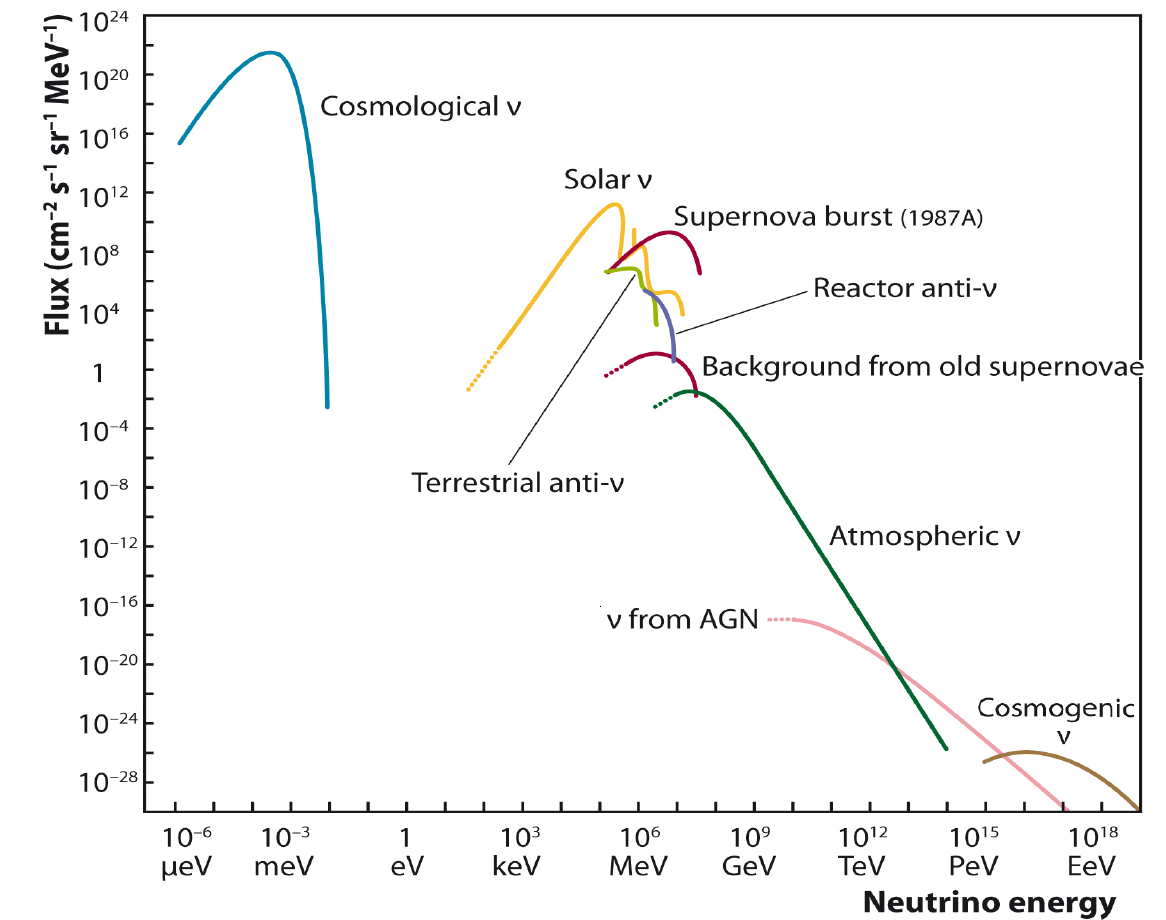
\includegraphics[width=0.7\textwidth]{Plots/neutrinoflux.png}
    \caption[Neutrinofluss in Abhängigkeit der Energie]{Neutrinofluss in Abhängigkeit der Energie für verschiedene Neutrinoquellen \cite{Spiering_2012}.
    }
    \label{fig:neutrino_flux}
\end{figure}

Der Neutrinofluss der energiereichsten Neutrinos ist so gering, dass zum Nachweis ein Detektor notwendig ist, der 1 bis 3 Größenordnungen größer als IceCube ist.
Wie in \autoref{fig:neutrino_flux} zu erkennen ist, handelt es sich bei den in IceCube detektierten Neutrinos um atmosphärische Neutrinos und Neutrinos aus aktiven Galaxiekernen (AGN).
\\
Atmosphärische Neutrinos entstehen bei der Kollision hochenergetischer Teilchen mit der Erdatmosphäre.
Kosmische Strahlung besteht überwiegend aus geladenen Kernen.
Diese wechselwirken mit den Atomkernen in der Atmosphäre und zerfallen über die schwache Wechselwirkung.
Es wird ein Neutrino frei.
\\
Ein Ziel von IceCube ist die Gewinnung neuer Erkenntnisse über die Quellen kosmischer Strahlung, in denen auch hochenergetische Neutrinos erzeugt werden.
\\
Es existieren drei Generationen (Flavor) von Neutrinos, das Elektron-Neutrino $\nu_e$, das Myon-Neutrino $\nu_\mu$ und das Tau-Neutrino $\nu_\tau$.
Aus Modellen, die verschiedene Neutrinoquellen betrachten geht hervor, dass Neutrinos im Verhältnis $\nu_e$:$\nu_\mu$:$\nu_\tau$ = $1$:$2$:$0$ entstehen.
Auf der Erde werden alle Neutrinos gleichermaße gemessen: $\nu_e$:$\nu_\mu$:$\nu_\tau$ = $1$:$1$:$1$.
Grund sind die Neutrino-Oszillationen\cite{oscillation_bilenky,oscillation_wolfenstein}, die einen Wechsel zwischen Generationen ohne weitere Wechselwirkung erlauben.
\\
Die drei Neutrinoarten erzeugen im Detektor unterschiedliche Signaturen und ermöglichen eine Bestimmung des Flavors.
Eine \textbf{Kaskade}\cite{signature_e} wird beobachtet, wenn bei der Wechselwirkung eines $\nu_e$ ein $e^{\pm}$ ensteht.
Aufgrund von Bremsstrahlungs- und Paarproduktionsprozessen nimmt die Energie ab.
Am Ort der Wechselwirkung befindet sich das Energiemaximum.
\\
Reagiert ein $\nu_\mu$ mit dem Eis, so entsteht als sekundäres Teilchen ein Myon $\mu$.
Dieses propagiert durch das Eis und verliert Energie in Form von Ionisation, Paarerzeugung, Bremsstrahlung und photonuklearen Wechselwirkungen.
Die Signatur entspricht einer \textbf{Spur} mit abnehmender Energie.
\\
Der \textbf{Double Bang} ("`Doppel-Knall"') wird durch ein $\nu_\tau$ hervorgerufen.
Bei der Wechselwirkung entsteht ein Tauon $\tau$ und es wird eine Kaskade erzeugt.
Der Zerfall des Tauons, nach der mittleren Lebensdauer von $\SI{290.3(5)e-15}{\second}$ \cite{pdg} führt zu einer weiteren Kaskade.
So ein Ereignis wäre ein klarer Nachweis für ein $\nu_\tau$.
\chapter{Entfaltung}
Vorerst wird das zugrundeliegende Problem in \autoref{sec:inverse_problem} aufgeführt und die Entfaltung diskutiert.
Im Anschluss wird in \autoref{sec:dsea} auf den Lösungsansatz mit DSEA eingegangen und der Algorithmus erläutert.
Das letzte Kapitel \autoref{sec:NN} befasst sich mit neuronalen Netzen und wie sie als Klassifikationsalgorithmus verwendet werden können.

% INVERSE PROBLEME
\section{Inverse Probleme} \label{sec:inverse_problem}
Inverse Probleme treten in der Physik überall da auf, wo die gesuchte physikalische Größe nicht \textit{direkt} messbar ist.
Die Neutrinoenergie ist nur \textit{indirekt} messbar.
Ziel ist die Rekonstruktion der gesuchten Größe, also der Neutrinoenergie aus der Messgröße.
In IceCube wird das Cherenkov-Licht der Zerfallsprodukte gemessen, siehe dazu \autoref{sec:icecube}.
\\
Mathematisch ist das Problem über die Fredholm-Integralgleichung\cite{twomey1963numerical} 
\begin{equation}
    \int_{\Omega} A(x,y) f(x) \mathrm{d}x + b(y) = g(y)
\end{equation}
definiert.
Die Verteilung des wahren Parameters $x$ wird durch $f(x)$ und die Verteilung der Messdaten durch $g(x)$ dargestellt.
Der gesamte Messprozess und die ablaufenden physikalischen Prozesse werden durch die Antwortfunktion $A(x,y)$ beschrieben.
Üblicherweise wird der Messprozess durch einen Untergrund $b(y)$ beeinflusst.
Dieser ist nicht von Interesse und kann mit Signal-Untergrund-Trennverfahren separiert werden.
\\
Im diskreten Fall werden die kontinuierlichen Verteilungen $f(x), g(y)$ zu \textbf{Vektoren} und $A(x,y)$ zu einer Antwort\textbf{matrix}.
Ohne Untergrund vereinfacht sich die Gleichung zu
\begin{equation}
    g_i = \sum_{j=1}^{n} A_{ij} f_j \, .
\end{equation}

Die Rekonstruktion der Größe $f$ wird als Entfaltung bezeichnet.
Der naive Ansatz über Bildung der Inverse von $A$ führt häufig zu unbrauchbaren Lösungen.
Kleine anfängliche Störungen verstärken sich und man erhält eine stark oszillierende Lösung.
Das Problem ist schlecht konditioniert und benötigt spezielle Ansätze.

% DSEA
\section{Lösungen mit DSEA} \label{sec:dsea}
Der \textbf{D}ortmund \textbf{S}pectrum \textbf{E}stimation \textbf{A}lgorithm (DSEA)\cite{ruhe,RockSolid2018DSEARR,boerner} betrachtet die Entfaltung als Klassifikationsproblem.
Vorab wird die Zielvariable $f(x)$ in $n$ Intervalle unterteilt:
\begin{equation}
    f(x) \rightarrow \vec{f}: \qquad f_j = \int_{y_{j-1}}^{y_j} f(x) \, \mathrm{d}x, \qquad j \in [1,n]
    \label{eq:diskretisierung}
\end{equation}
Jedes Intervall bzw. jeder Bin repräsentiert den in \autoref{eq:diskretisierung} definierten Energiebereich.
Die Bins stellen in DSEA die Zielklassen für eine Klassifikation dar.
\\
\\
DSEA ist ein iteratives Verfahren.
Im ersten Schritt wird ein Klassifikationsalgorithmus auf dem Datensatz ($X,W,F$) trainiert.
Dabei steht $X$ für die Features, die mit den Probengewichten $W$ gewichtet werden und $F$ für das Label.
DSEA geht von Daten mit gleichverteilten Klassen aus, d.h. die Gewichte $W$ werden dementsprechend initialisiert.
Dies hat den Vorteil, dass kein Prior angenommen werden muss und somit das Modell unabhängig von der Klassenverteilung im Trainingsdatensatz ist.
\\
Voraussetzung an den Klassifizier ist, dass dieser eine Konfidenz $c_{ij}$ ausgibt, die die Zugehörigkeit des $i$-ten Events zum $j$-ten Bin beschreibt.
Die Konfidenz wird als Wahrscheinlichkeit interpretiert.
\\
\\
Anschließend wird im 2. Schritt mit dem trainierten Klassifizierer/Modell eine Vorhersage für die zu entfaltenden Daten getroffen.
Über die für jedes Event $i$ und Bin $j$ erhaltende Konfidenz wird das Spektrum
\begin{equation}
    \hat{f}_{j} = \sum_{i=1}^{n} c_{ij}
    \label{eq:dsea_confidence}
\end{equation}
rekonstruiert, wobei $n$ die Anzahl der Datenpunkte angibt.
Die Konfidenzen werden für jeden Bin $j$ über alle Events aufsummiert und man erhält eine Vorhersage für den $j$-ten Bin des zu entfaltenden Spektrums $\hat{f}_j$.
\\
Im letzen (3.) Schritt werden die Probengewichte $w_{i}$
\begin{equation}
    w_{i} = \frac{f_{l_i}}{n}
\end{equation}
über das rekonstruierte Spektrum aktualisiert, wobei $l_i$ dem wahren Label des $i$-ten Events entspricht.
Die Gewichte entsprechen dem normierten Spektrum.
\\
Die erste DSEA-Iteration ist hiermit vollendet.
Anschließend wird wieder Schritt 1 ausgeführt und der Klassifizier mit angepassten Probengewichten trainiert.
Es werden soviele Iterationen ausgeführt bis Konvergenz eintritt.


% NEURONALE NETZE
\section{Neuronale Netze als Klassifikationsalgorithmus} \label{sec:NN}
Grundsätzlich kann jeder Klassifizierer verwendet werden, der für jede Zielklasse eine Konfidenz $c_{ij}$ ausgibt.
Beliebte Klassifikationsalgorithmen in DSEA sind Naive Bayes oder auch der Random Forest.
In dieser Arbeit werden neuronale Netze (\textbf{NN}) als Klassifizier in DSEA untersucht.
\begin{figure}
    \centering
    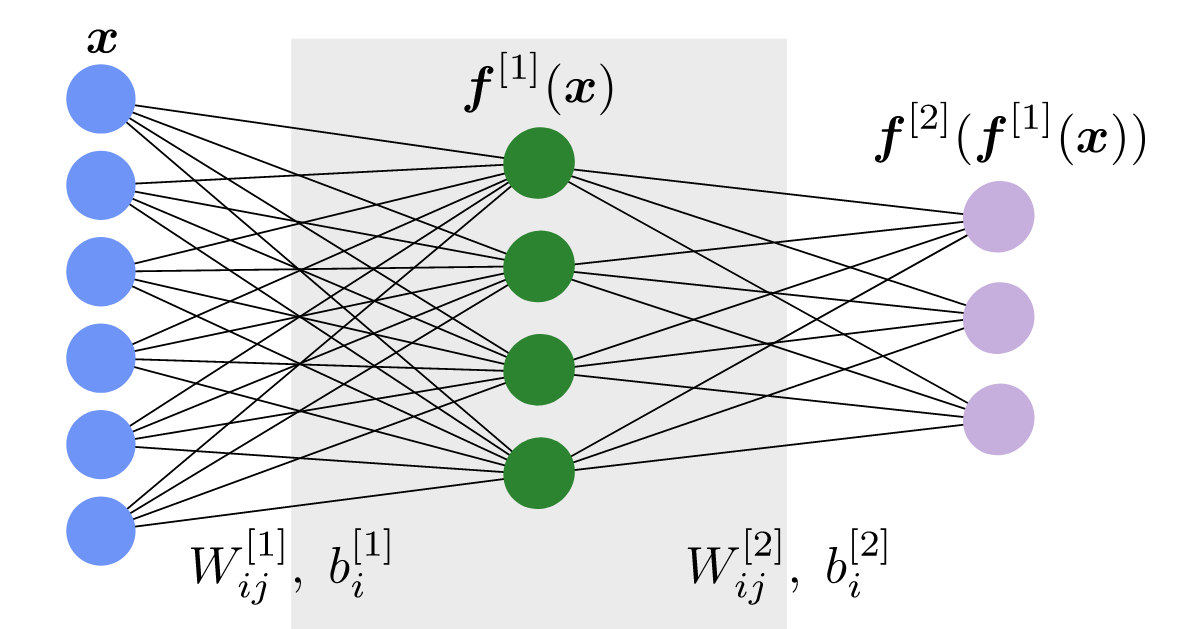
\includegraphics[width=0.8\textwidth]{Plots/nn_structure.png}
    \caption[Struktur eines NN mit einer tiefen Ebene]{Darstellung der Struktur eines einfachen neuronalen Netzes.
    Die blauen Kreise stellen die Neuronen der Eingansebene, die Grünen der tiefen Ebene und die Blauen der Ausgangsebene dar.
    Jedes Neuron besitzt zwei Parameter, eine Gewichtsmatrix $\mathbf{W}_{ij}$ und einen Biasvektor $\vec{b}_i$.
    Das Resultat für jede Ebene wird durch $f(x)$ beschrieben \cite{Neupert2021IntroductionTM}.
    }
    \label{fig:nn_structure}
\end{figure}
Das NN in \autoref{fig:nn_structure} beinhaltet drei Ebenen, wobei jede Ebene eine bestimmte Anzahl an Neurononen enthält.
Die Eingangsebene (Blau) besteht aus so vielen Neuronen, wie Features verwendet werden.
Jedes Neuron erhält also als Eingang ein Feature.
Es können beliebig viele tiefe Ebenen (Grün) verwendet werden.
Die Verbindungen zwischen zwei Ebenen wird durch die Gewichtsmatrix $\mathbf{W}$, den Biasvektor $\vec{b}$ und einer Aktivierungsfunktion $g(\vec{x})$ nach
\begin{equation*}
    g(f(\vec{x})) = g(\mathbf{W} \vec{x} + \vec{b})
\end{equation*}
beschrieben, wobei $\vec{x}$ den Ausgang aus der vorherigen Ebene beschreibt.
Es gibt eine große Auswahl an Aktivierungsfunktionen\cite{activationf}.
\begin{figure}
    \centering
    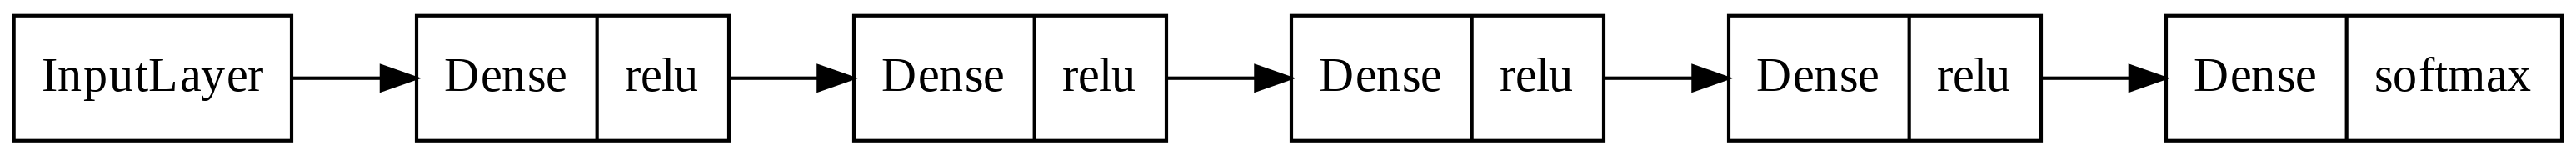
\includegraphics[width=\textwidth]{Plots/model_structure.png}
    \caption[Aufbau des verwendeten NN]{Der Aufbau des NN schematisch dargestellt.
    Nach der Eingangsebene folgen mehrere tiefe Ebenen mit der Aktivierungsfunktion ReLU.
    Die Verbindungen der letzten Ebene werden durch die Softmax-Funktion definiert.
    \label{fig:nn_aufbau}
    }
\end{figure}
Große NN mit vielen Parametern haben den Nachteil sich stark an die Daten anzupassen (Bias).
Bei dem in dieser Arbeit verwendeten NN handelt es sich um ein tiefes neuronales Netz mit etwa $\SI{60000}{\text{Parametern}}$.
Die Struktur ist in \autoref{fig:nn_aufbau} graphisch dargestellt.
Für quantitative Angaben der Ein- und Ausgangsdimensionen siehe \autoref{tab:nn_shape}.
Der einfache Aufbau soll zu einem geringen Bias im Modell führen.
\\
In den tiefen Ebenen wird die Aktivierungsfunktion \textit{ReLU} (\textbf{Re}ctified \textbf{L}inear \textbf{U}nit)
\begin{equation*}
    g_\text{ReLU}(x)=
        \begin{cases}
            x & {\text{if }} x \geq 0,\\
            0 & {\text{otherwise}}
        \end{cases}
\end{equation*}
genutzt.
Ist der Eingang $x$ größer 0, so wird dieser unverändert weitergegeben, sonst 0.
\\
Die Ausgangsebene enthält genauso viele Neuronen, wie es Zielklassen gibt.
In dieser Ebene wird die Aktivierungsfunktion Softmax verwendet.
Wie die Definition
\begin{equation*}
    g_\text{Softmax}(x_i) = \frac{\exp(x_i)}{\sum_j \exp(x_j)} \, .
\end{equation*}
zeigt, ist die Summe über alle Klassen für jedes Event gleich eins.
Sie erfüllt damit die Vorgabe an DSEA, dass für jede Zielklasse eine Konfidenz $c_{ij}$ ausgegeben wird.
\\
Die Kostenfunktion \textit{kategorische Kreuzentropie}\cite{cross_entropy} kann für ein Klassifikationsproblem verwendet werden.
Ziel ist die Minimierung der Kosten in Abhängigkeit der Modellparameter.
Die Minimierung der Kreuzentropie ist äquivalent zu einer Maximierung der Log-Likelihood-Funktion.
\\
Mit dem Optimierer \textit{ADAM} (Adaptive Moment Estimation)\cite{ADAM} wird die Kostenfunktion minimiert.
Der Algorithmus ist eine Erweiterung des Gradientenverfahrens und beachtet zusätzlich zu der Steigung das Moment.
Bildlich gesehen entspricht dies einer Kugel, die in einer hügeligen Landschaft Richtung globalem Minimum rollt und dabei lokale Minima überwindet.
Die Lernrate stellt ein Hyperparameter des Optimierers dar und ist ein Maß für die Schrittweite entlang des fallenden Gradienten.
\\
Das Modell wird auf einem Teil der Daten trainiert und evaluiert.
Dazu wird der Datensatz in mehrere Unter-Datensätze mit einer spezifizierten Größe (\textit{Batch Size})\cite{brownlee2018difference} unterteilt.
Das Modell wird auf einem Batch trainiert und die Kostenfunktion ausgewertet.
Wird dies für alle Batches durchgeführt, so wurde jeder Datenpunkt im Training einmal berücksichtigt.
Durch das häufige Anpassen der Parameter konvergiert die Kostenfunktion schneller.
\\
Das Modell wird mehrfach auf den Trainingsdaten trainiert.
Die Anzahl der Trainingsprozesse wird durch die \textit{Epochenzahl}\cite{brownlee2018difference} angegeben.
\chapter{Verwendete Methoden}
In diesem Kapitel werden die verwendeten Methoden vorgestellt.
\autoref{sec:chi2} behandelt die $\Chi^2$-Distanz als Abstandsmaß zweier diskreter Verteilungen.
In \autoref{sec:bootstrap} wird die Berechnung der Unsicherheiten mithilfe von Bootstrapping erläutert.

\section{Chi-Quadrat-Distanz} \label{sec:chi2}
Die $\chi^2$-Distanz\cite{LIU20022617} ist ein gewichtetes Abstandsmaß und dient zur Überprüfung von Konvergenz.
Der Abstand zwischen der wahren Verteilung $f$ und der rekonstruierten Verteilung $\hat{f}$ wird über die Abstände der einzelnen Bins $j$ nach
\begin{equation}
    \chi^2 = \frac{1}{2} \sum_{j=1}^{n} \frac{(\hat{f}_j - f_j)^2}{\hat{f_j} + f_j}
\end{equation}
bestimmt.
Ist die $\chi^2$-Distanz kleiner oder gleich der $\chi^2$-Distanz in der vorherigen DSEA-Iteration, kann das Verfahren abgebrochen werden.

\section{Bootstrapping: Abschätzung der Unsicherheiten} \label{sec:bootstrap}
Bootstrapping\cite{lewis_poole_2004} ist eine Methode zur Bestimmung der Unsicherheiten von Wahrscheinlichkeitsmodellen.
Sie ist sinnvoll, wenn normalerweise nur ein kleiner Teil des Trainingsdatensatzes entfaltet wird.
\\
Die Methode beruht auf dem "`Resampling"', also einer Veränderung des ursprünglichen Datensatzes durch Mehrfachzählung und Nichtbeachtung von Events.
\\
\\
In \textbf{Schritt 1} wird der Datensatz durch Ersetzung von Events variiert.
Dieser Datensatz wird in \textbf{Schritt 2} mit DSEA (siehe \autoref{sec:dsea}) entfaltet.
In \textbf{Schritt 3} wird das entfaltete Spektrum gespeichert.
Die Schritte 1-3 werden $n$-mal wiederholt.
\\
\\
Anschließend kann die Verteilung jedes einzelnen Energie-Bins untersucht werden.
Zur Bestimmung des Mittelwerts kann der Median 
\begin{equation}
    \tilde {x} =
    \begin{cases}
        x_{m+1} & \text{ ,für ungerades n = 2m+1}\\
        \frac{1}{2} (x_{m}+x_{m+1}) & \text{ ,für gerades n = 2m}
    \end{cases}
\end{equation}
für jeden Energie-Bin berechnet werden, wobei $n$ die Anzahl der Entfaltungen angibt.
Die zugehörigen Unsicherheiten können allgemein über das untere und obere Quantil angegeben werden.
Das untere Quantil beinhaltet $\SI{16}{\percent}$ und das obere Quantil $\SI{84}{\percent}$ der Datenpunkte.
Zwischen den Quantilen liegen also $~\SI{68}{\percent}$ der Messwerte.
\\
Handelt es sich um normalverteilte Daten, so sind die Quantile äquivalent zu der Standardabweichung und der Median ist gleich dem Mittelwert.
\chapter{Testen der Hyperparameter in DSEA und neuronalen Netzen}
In diesem Kapitel werden die Ergebnisse präsentiert und diskutiert.
Vorerst wird der verwendete Datensatz charakterisiert und die Schritte der Daten-Vorverarbeitung beschrieben.
In \autoref{sec:nn_no_dsea} wird die Entfaltung über eine Klassifikation mit einem NN analysiert.
Ebenfalls wird bereits das Spektrum über die Aufsummierung der Konfidenzen rekonstruiert.
Hinzu kommt die iterative Anpassung der Gewichte, in \autoref{sec:deconv_dsea}.
Es werden neuronale Netze in DSEA systematisch über eine Gittersuche analysiert.
Anschließend wird der Trainingsprozess, die entfalteten Spektren und Korrelationen betrachtet.
Zum Schluss, wird in \autoref{sec:bias} die Abhängigkeit der Modelle vom Trainingsspektrum untersucht.

\section{Datensatz}
Der Monte-Carlo Datensatz 11374 \cite{dataset} beinhaltet Neutrinos mit einem simulierten Spektrum $E^{-2}$.
Es werden nur sog. "`upgoing"'  Neutrinos betrachtet.
Das sind Neutrinos die vor der Detektion die Erde durchquert haben.
Es wurde bereits eine Eventauswahl durchgeführt.
\begin{table}
    \centering
    \caption{Statistische Kennzahlen zu der Energie des primären Neutrinos.
    Links für die ursprünglichen MC-Daten (Rohdaten) und im direkten Vergleich, der abgeschnittene Datensatz mit Energien $\leq \SI{100}{\tera\eV}$ (rechts).
    }
    \label{tab:energy_stats}
    \begin{tabular}{l|c c}
        \toprule
        & Rohdaten & Daten nach Schnitt \\
        \midrule
        Anzahl Events & $\SI{1.334e+7}{}$ & $\SI{1.326e+7}{}$\\
        Mittlere Energie $\mu$ & $\SI{6.3}{\tera\eV}$ & $\SI{2.2}{\tera\eV}$ \\
        Standardabweichung $\sigma$ & $\SI{246}{\tera\eV}$ & $\SI{7}{\tera\eV}$ \\
        Minimum & $\SI{100}{\giga\eV}$ & $\SI{100}{\giga\eV}$ \\
        Maximum & $\SI{e+8}{\giga\eV}$ & $\SI{e+5}{\giga\eV}$ \\
        $\SI{25}{\percent}$-Quantil & $\SI{271}{\giga\eV}$ & $\SI{270}{\giga\eV}$ \\ 
        $\SI{50}{\percent}$-Quantil & $\SI{547}{\giga\eV}$ & $\SI{543}{\giga\eV}$ \\ 
        $\SI{75}{\percent}$-Quantil & $\SI{1.42}{\tera\eV}$ & $\SI{1.39}{\tera\eV}$ \\ 
        \bottomrule
    \end{tabular}
\end{table}
Dazu wird der Zenitwinkel mit einem Fehler von \SI{5}{\degree} rekonstruiert und Events von \SIrange{86}{180}{\degree} beibehalten.
Dies hat den Vorteil, dass keine Signaturen von Myonen beachtet werden müssen.
Die Myonen wechselwirken mit der Erde und können den Detektor nicht erreichen.
Anders als für Myonen, stellt die Erde für Neutrinos kein Hindernis dar.
Aufgrund des geringen Wirkungsquerschnitts erreichen die meisten Neutrinos den Detektor.
Der Datensatz beinhaltet 13 Millionen Events.
Die Energie des primären Neutrinos stellt die Zielvariable des Klassifikationsproblems dar.
In \autoref{tab:energy_stats} sind wichtige Informationen über die Lage und Streuung der Neutrinoenergie aufgeführt.
%%%%%%%
Auffällig ist, dass der größte Teil der Events im niederenergetischem Bereich liegt.
Augrund der geringen Statistik im Hochenergiebereich werden nur Events unter $\SI{100}{\tera\eV}$ berücksichtigt.
Die untere Energiegrenze bleibt unverändert und beträgt $\SI{100}{\giga\eV}$.
Mit einer logarithmischen Skala wird die Energie in 10 Klassen aufgeteilt.
Das logarithmische Binning kompensiert zum Teil die wenigen Events im Hochenergiebereich.
Wird mit realen Daten gearbeitet, so können an dieser Stelle Under- und Overflow-Bins eingeführt werden.
Diese decken den für die Analyse nicht-relevanten Bereich ab.
$\SI{90}{\percent}$ der Events werden zum Trainieren und die restlichen Events zur Evaluation des Modells verwendet.
\\
Die 12 Features (siehe \autoref{tab:feature}) werden vor der Entfaltung normalisiert
\begin{equation*}
    z = \frac{x-\mu}{\sigma}
\end{equation*}
um gleiche Abstände zwischen den Features zu gewährleisten.
Dies ist ein notwendiger Schritt zur Optimierung des Trainingsprozesses \cite{scaler}.

% NN OHNE DSEA
\section{Entfaltung als Klassifikationsproblem} \label{sec:nn_no_dsea}
Die Betrachtung der Entfaltung als Klassifikationsproblem ist eine der grundlegenden Ideen von DSEA.
In diesem Kapitel soll vorerst die Entfaltung über eine klassische Klassifikation diskutiert werden.
Die \autoref{fig:single_event} zeigt exemplarisch die Vorhersage eines einzelnen Events.
Die Zugehörigkeit des Events zum $j$-ten Energie-Bin wird durch die Konfidenz $c_j$ angegeben.
Ein Datenpunkt wird nach dem Prinzip \textit{maximum a posterioro} der Klasse mit der \textbf{maximalen Konfidenz} zugeordnet \cite{max_pred}:
\begin{equation*}
    \hat{y} = \underset{j}{\arg\max} \{ c_j \}, \qquad j=[0,...,n-1]
\end{equation*}
Die Anzahl der Energie-Bins ist über $n$ definiert.
Das NN wird auf den Trainingsdaten mit \SI{50}{\text{Epochen}} trainiert.
In \autoref{tab:nn_params} sind die verwendeten Hyperparameter des NN aufgeführt.
\SI{500000}{\text{Events}} der Evaluationsdaten werden entfaltet und analysiert.
Ein Event wird jeweils der maximal vorhergesagten Klasse zugeordnet.
Die Kostenfunktion, sowie die Metriken werden in jeder Epoche im Trainingsprozess für die Trainings- und Evaluationsdaten ausgewertet.
Der Verlauf der kategorischen Kreuzentropie und der $\Chi^2$-Distanz ist in \autoref{fig:NN_history} dargestellt.
\\
\begin{wrapfigure}{l}{.5\textwidth} %[17]{l}{.5\textwidth}
    \centering
    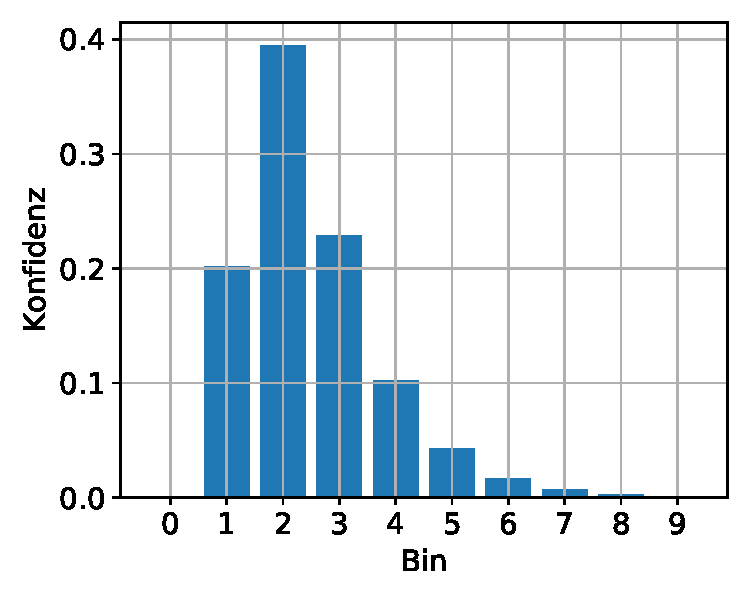
\includegraphics[width=.5\textwidth]{Plots/NN/single_events_class2.pdf}
    \caption[Graphische Darstellung der Ausgabe des NN]{Visuelle Darstellung der Ausgabe des NN für ein Event mit der wahren Energieklasse 2.
    Die Zugehörigkeit des Events zu Bin $j$ ist durch die Konfidenz $c_j$ definiert.
    }
    \label{fig:single_event}
\end{wrapfigure}
Die $\Chi^2$-Distanz, als Abstandsmaß zwischen dem wahren und vorhergesagten Spektrum konvergiert.
Ebenso verläuft der Verlust der Evaluationsdaten gegen ein Minimum.
Der Anstieg des Trainingsverlusts deutet auf ein leichtes Overtraining ("`Übertrainieren"') hin.
Eine Fortsetzung des Trainings ist daher nicht sinnvoll.
Das resultierende Spektrum in \autoref{fig:NN_spectrum_hard} weist starke Abweichungen von der wahren Verteilung auf.
Bins im hochenergetischen Bereich werden stark unterschätzt, hingegen werden die Bins bis etwa \SI{1}{\tera\eV} überschätzt.
Aufgrund der geringen Accuracy von $\sim\SI{39}{\percent}$ kommt es zu vielen Fehlklassifikationen.
Siehe dazu den Verlauf der Accuracy im Trainingsprozess \autoref{fig:NN_acc}.
Die Korrelation zu ähnlichen Energien bzw. benachbarten Bins wird hier nicht berücksichtigt.
\begin{figure}%
    \begin{subfigure}{0.5\textwidth}%
        \centering%
        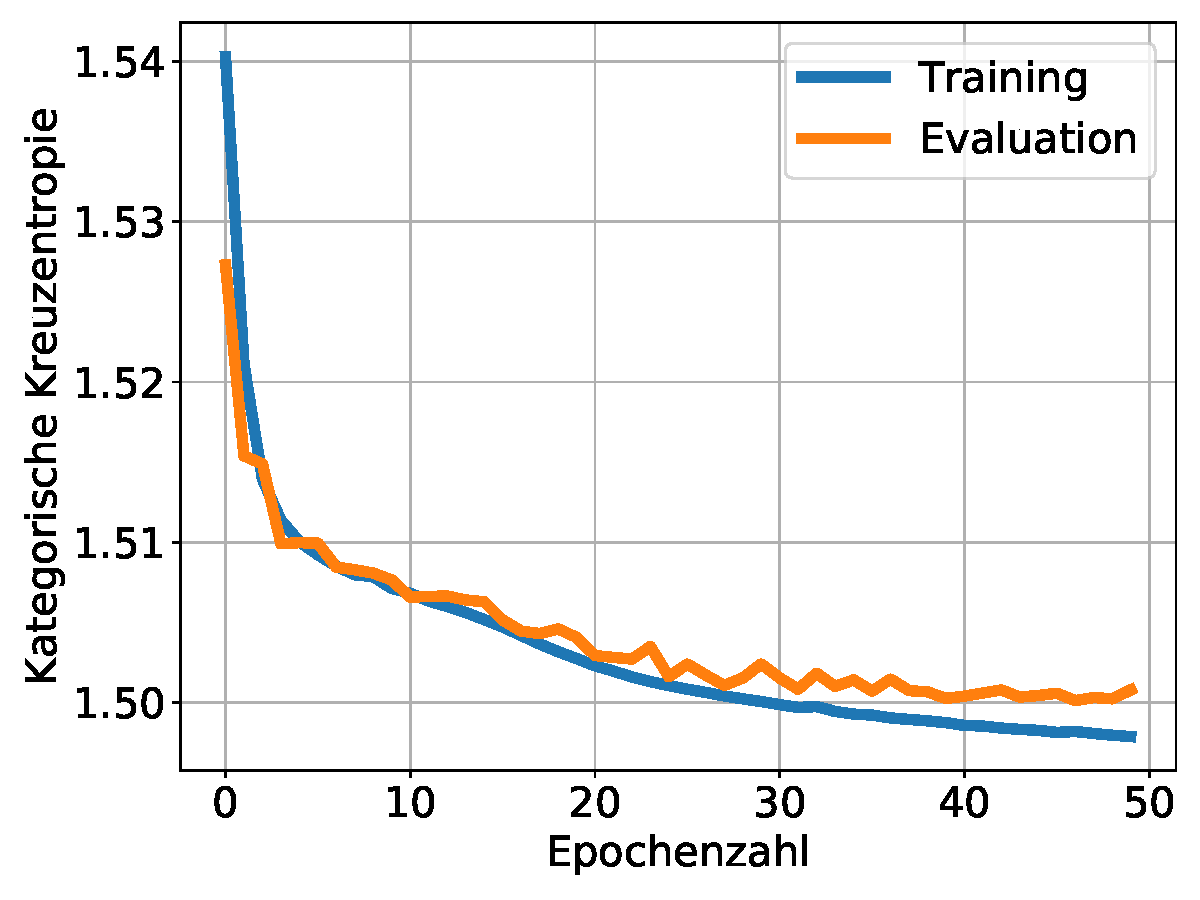
\includegraphics[height=5cm]{Plots/NN/loss.pdf}%
        \caption{Kostenfunktion: Kategorische Kreuzentropie}%
        \label{fig:NN_loss}%
    \end{subfigure}%
    \hfill% Fills available space in the center -> space between figures
    \begin{subfigure}{0.5\textwidth}%
        \centering%
        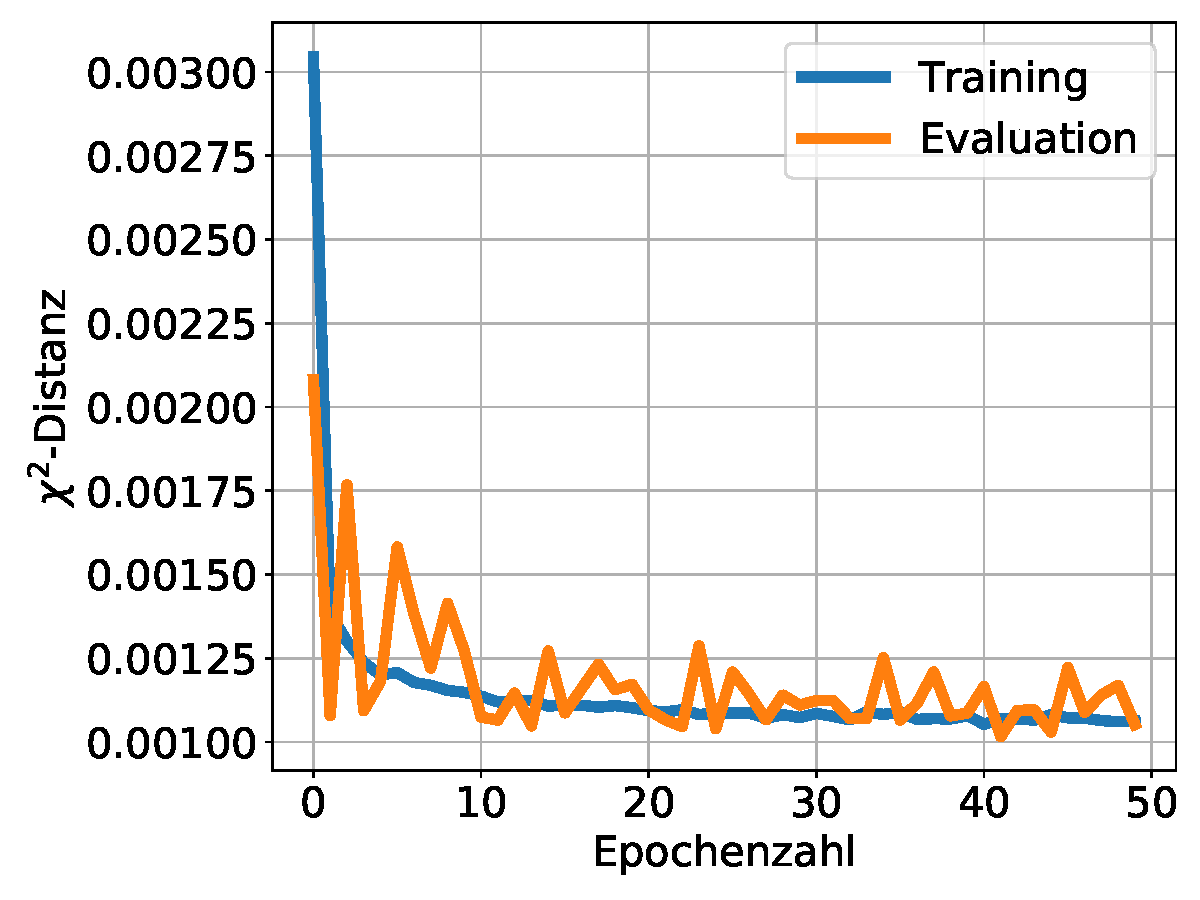
\includegraphics[height=5cm]{Plots/NN/chi.pdf}%
        \caption{Metrik: $\Chi^2$-Distanz}%
        \label{fig:NN_chi}%
    \end{subfigure}%
    \caption[Verlauf des Trainingsprozesses des NN ohne DSEA]{Verlauf des Trainingsprozess des NN.
    Zum einen ist die Kostenfunktion \textit{kategorische Kreuzentropie} und zum anderen die \textit{Chi-Quadrat-Distanz} als Metrik in Abhängigkeit der Epochenzahl aufgeführt.
    }
    \label{fig:NN_history}%
\end{figure}%

\begin{figure}
    \centering
    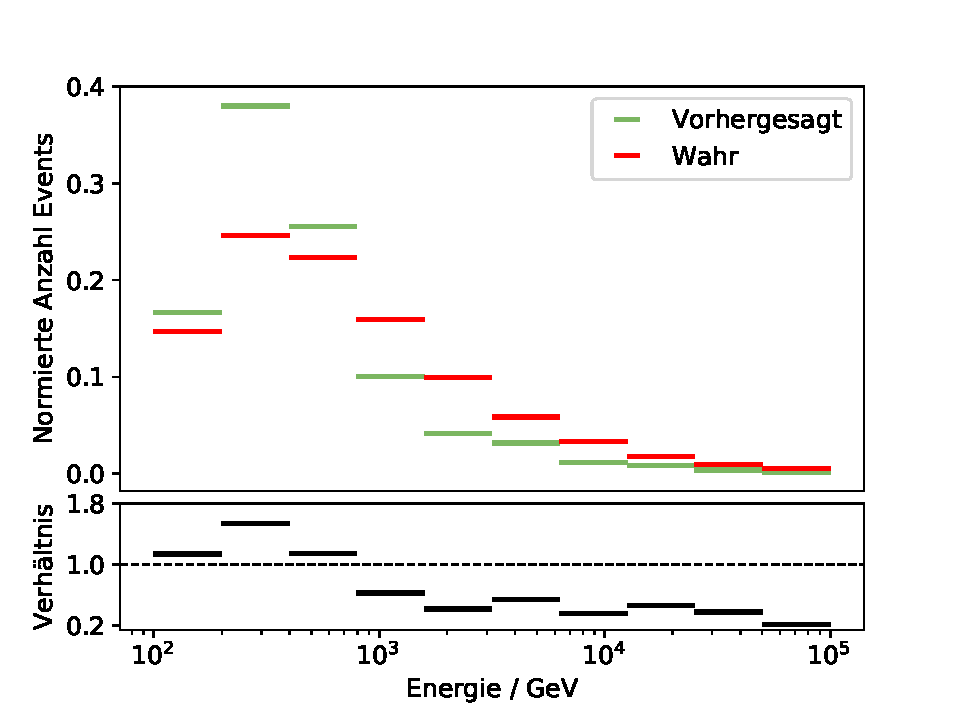
\includegraphics[width=\textwidth]{Plots/NN/spectrum_hard_10bins_50ep_500000samples_200pulls.pdf}
    \caption[Spektrum des NN ohne DSEA bei einer Klassifikation nach dem "`maximum a posterioro"'-Prinzip]{Das vorhergesagte und wahre Spektrum für ein NN, wenn ein Event der maximal vorhergesagten Klasse zugeordnet wird.
    Der untere Teil zeigt das Verhältnis zwischen wahrem und vorhergesagtem Spektrum und ist ein Maß für die relative Abweichung.
    Energien bis etwa \SI{1}{\tera\electronvolt} werden systematisch überschätzt, wobei die hochenergetischen Events unterschätzt werden.
    }
    \label{fig:NN_spectrum_hard}
\end{figure}
Die zweite grundlegende Idee die DSEA definiert, ist die \textbf{Wahrscheinlichkeitsinterpretation} der Konfidenzen $c_{ij}$.
Anstatt die Klasse mit der größten Konfidenz zu wählen, werden die Konfidenzen für jede Zielklasse aufsummiert (\autoref{eq:dsea_confidence}).
Die \autoref{fig:NN_spectrum} zeigt das resultierende Spektrum mit zugehöriger Abweichung.
\begin{figure}
    \centering
    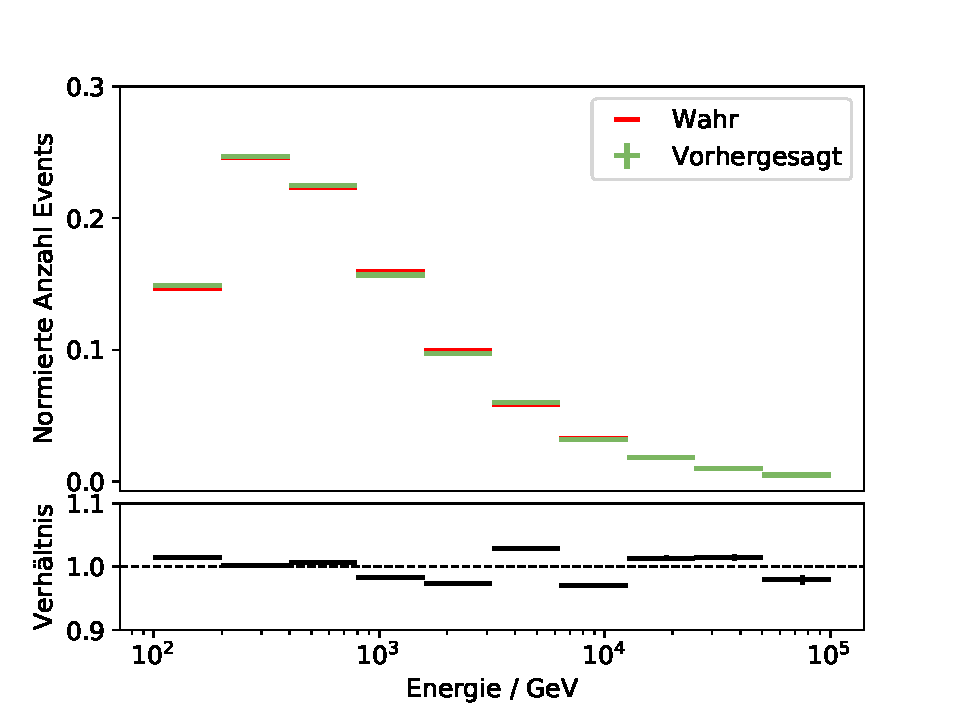
\includegraphics[width=0.9\textwidth]{Plots/NN/spectrum_dist_10bins_50ep_500000samples_200pulls.pdf}
    \caption[Spektrum des NN ohne DSEA mit Beachtung der Wahrscheinlichkeitsinterpretation]{Vorhergesagtes und wahres Spektrum für ein NN, wenn die Konfidenzen für jeden Bin aufsummiert werden.
    Der untere Teil zeigt das Verhältnis zwischen wahrem und vorhergesagtem Spektrum und dient als Maß für die relative Abweichung.
    Bestimmung der Unsicherheiten über das Bootstrapping-Verfahren, siehe \autoref{sec:bootstrap}.
    }
    \label{fig:NN_spectrum}
\end{figure}
Die Vorhersage stimmt hier weitgehend mit dem wahren Spektrum überein, wie auch der Verhältnis-Plot zeigt.
Größere Abweichungen sind in den Hochenergie-Bins zu beobachten.
Dort treten auch die für eine Entfaltung typischen Oszillationen auf.
\\
\\
Wie die Vorhersage einzelner Events (\autoref{fig:NN_single_events}) andeutet, wird durch die in \autoref{fig:nn_correlation} dargestellte Korrelationsmatrix bestätigt.
Es gibt eine starke Korrelation zwischen benachbarten Bins.
Grund dafür ist die ordinale Natur des Problems.
Jede Klasse repräsentiert bestimmte Energien, die einer definierten Ordnung folgen.
\begin{figure}
    \centering
    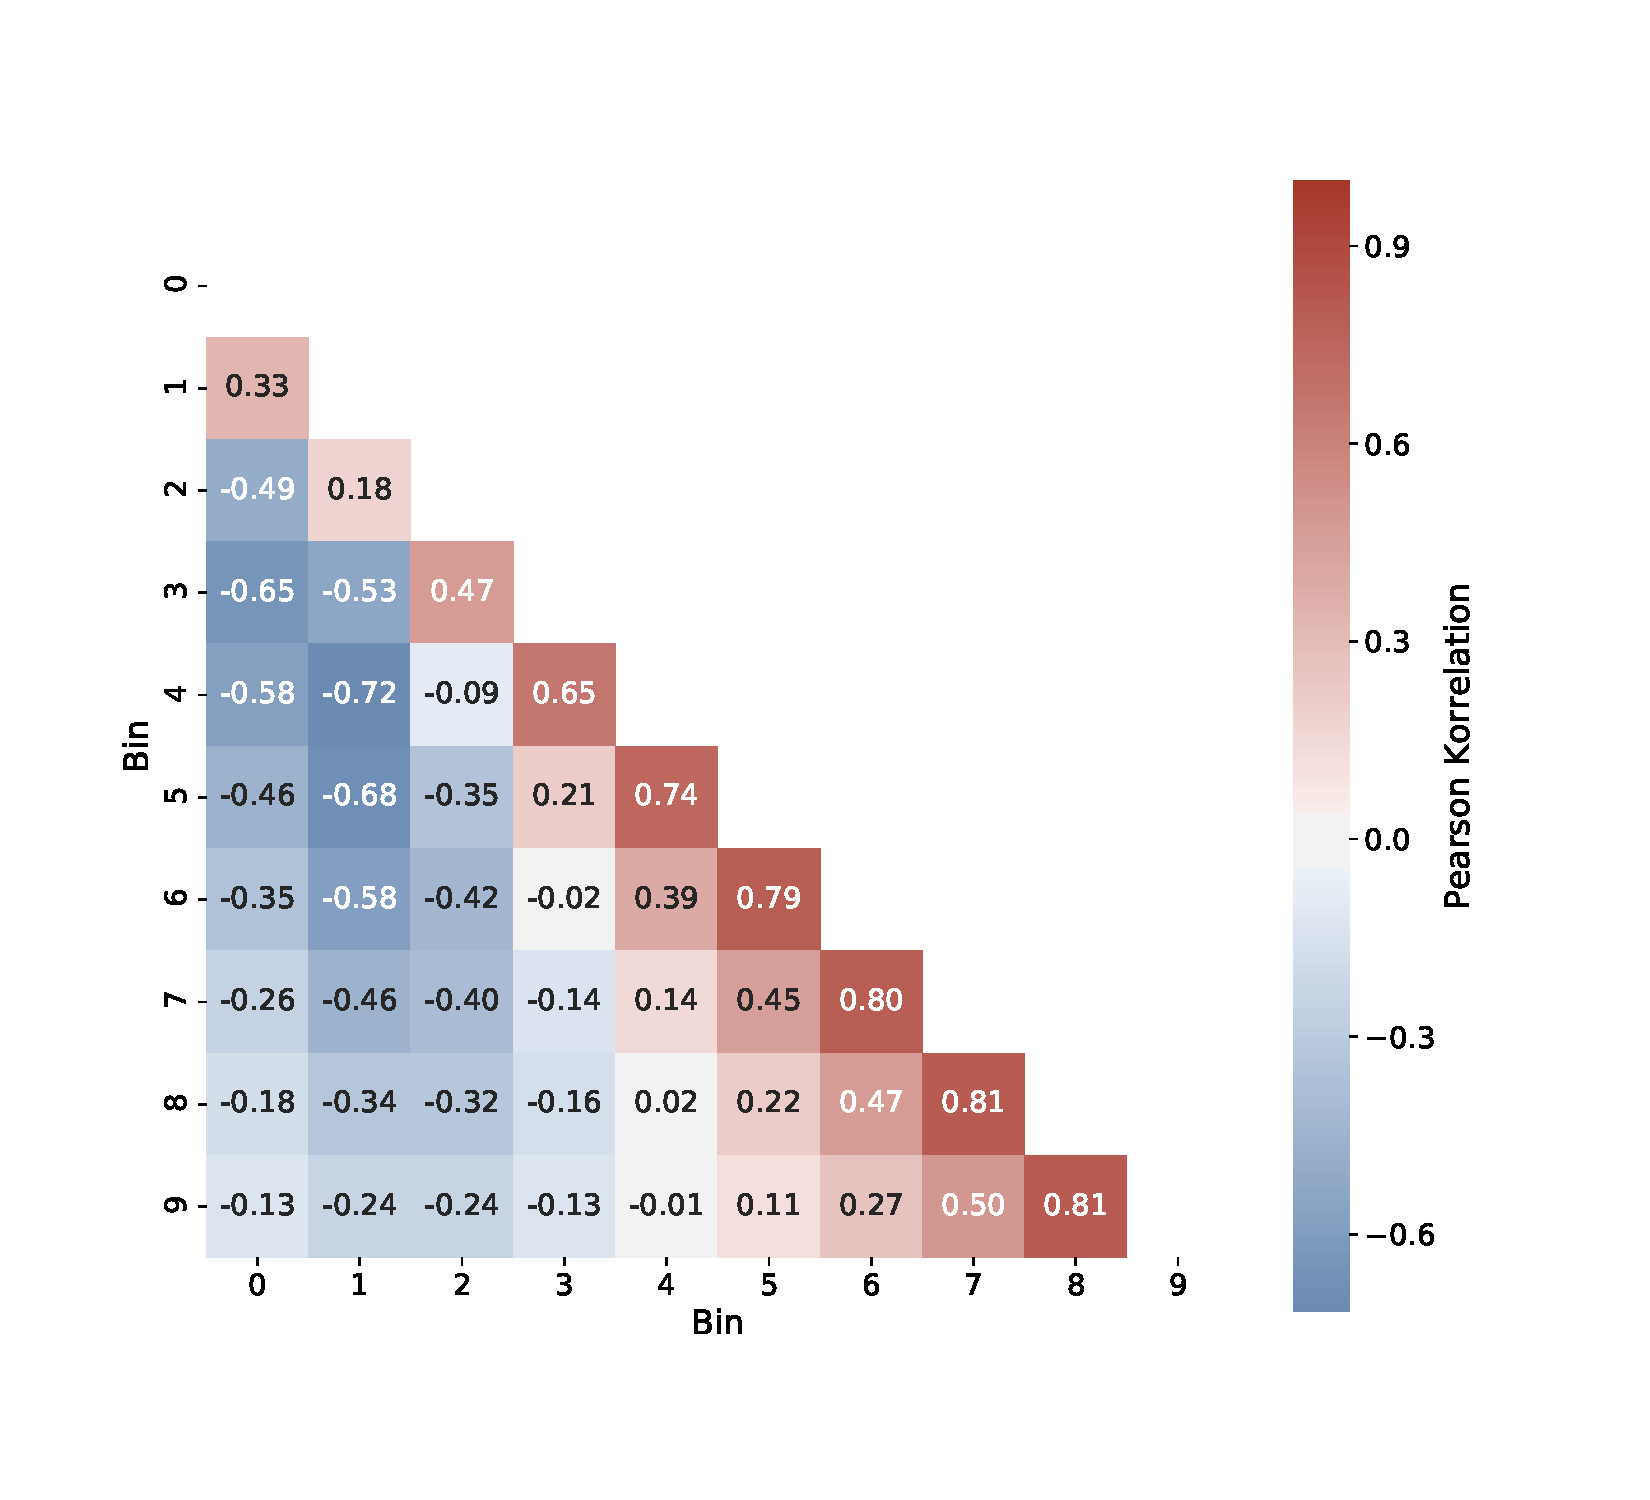
\includegraphics[width=\textwidth]{Plots/NN/correlation_matrix.pdf}
    \caption[Korrelationsmatrix des NN ohne DSEA]{Darstellung der relevanten Komponenten der symmetrischen Korrelationsmatrix.
    Sie gibt die Korrelationen zwischen den \SI{10}{\text{Bins}} für das NN an.
    }
    \label{fig:nn_correlation}
\end{figure}

% NN IN DSEA
\section{Entfaltung mit DSEA} \label{sec:deconv_dsea}
\subsection{Initialisierung}
DSEA ist für Klassifikationsalgorithmen der Scikit-Learn-Bibliothek\cite{scikit-learn} ausgerichtet.
Diese ist nicht für die Implementierung neuronaler Netze optimiert.
In der Arbeit wird dazu das Framework \textit{Tensorflow}\cite{tensorflow2015-whitepaper} und dessen API \textit{Keras} verwendet.
\\
Statt den Quellcode von DSEA anzupassen, wird ein Wrapper ("Verpackung") für die Keras-API entwickelt.
Der Wrapper kann im Anhang \ref{code:wrapper} eingesehen werden.
\\
Die Methoden \textit{fit()} und \textit{predict()} sind, wie die Methoden der Klassifizierer der Scikit-Learn-Bibliothek aufgebaut.
Die Konsequenz ist, dass bereits bei der Initialisierung die Hyperparameter übergeben werden.
Das sind Parameter die üblicherweise in der \textit{fit()} Methode auftreten. 
Betroffen sind die Anzahl der Epochen, Batchgröße und die Lernrate.
\\
Der neu eingeführte Parameter \textbf{one\_model} $[$Bool$]$ gibt an, ob im gesamten Trainingsprozess nur ein Modell verwendet wird:

\begin{description}
    \item [True]Ein Modell wird trainiert, wobei die Gewichte in jeder DSEA-Iteration aktualisiert werden
    \item [False]In jeder DSEA-Iteration wird ein neues Modell erstellt, welches auf den angepassten Gewichten trainiert wird
\end{description}
Die meisten Klassifizierer basieren nicht auf einer Verlustfunktion und können somit den Trainingsprozess nicht fortsetzen.
Das bedeutet, dass die Klassifizierer der Scikit-Learn-Bibliothek in jeder DSEA-Iteration neu initialisiert werden.
NN in DSEA bieten also die Freiheit, zwischen den beiden Szenarien zu wählen.
\\
Die Anzahl an Epochen pro DSEA \textit{Iteration} ist durch den Parameter \textit{Epochen} definiert.
Die Gesamtanzahl der Epochen ergibt sich durch \textit{Epochen} $\times$ \textit{Iterationen}.

% Gridsearch
\subsection{Optimierung der Hyperparameter}
Zur systematischen Untersuchung der drei Parameter \textit{Anzahl Epochen}, \textit{Anzahl Iterationen in DSEA} und \textit{one\_model} wird eine Gittersuche durchgeführt.
Es wird das bereits bekannte Modell \ref{tab:nn_shape} mit der gleichen Batchsize und Lernrate verwendet.
Aufgrund der Rechenzeit wird für die Gittersuche nur ein Teil des Trainingsdatensatzes mit $\sim \SI{1000000}{\text{Events}}$ genutzt.
\\
Zur Evaluation der Modelle werden die Abstände zwischen dem wahren und entfalteten Spektrum betrachtet.
Es werden $\sim \SI{500000}{\text{Events}}$ entfaltet und ausgewertet.
In \autoref{tab:gridsearch} sind die Parameter der 10 besten Modelle der Gittersuche, nach der $\Chi^2$-Distanz sortiert, aufgelistet.

\begin{table}
    \centering
    \caption{Die 10 besten Modelle der Gittersuche für die Parameter \textit{Anzahl Epochen}, \textit{Anzahl Iterationen in DSEA} und \textit{one\_model} aufgeführt. Die Ergebnisse sind nach der $\Chi^2$-Distanz sortiert. Ebenfalls ist der Root Mean Square Error (RMSE) angegeben.}
    \label{tab:gridsearch}
    \begin{tabular}{l l l | l l}
        \toprule
        Epochen & Iterationen &	one\_model & RMSE & $\Chi^2$-Distanz \\
        \midrule
        \rowcolor{tugreen}
        $75	$ & $12$ & False & $0.003123$ & $0.000269$ \\
        \rowcolor{tugreen}
        $60	$ & $16$ & True & $0.003282$ & $0.000293$ \\
        $50	$ & $16$ & True & $0.004092$ & $0.000439$ \\
        $50	$ & $8$ & False & $0.004332$ & $0.000449$ \\
        $10	$ & $12$ & True & $0.005303$ & $0.000518$ \\
        $100$ & $20$ & False & $0.006635$ & $0.000623$ \\
        $25	$ & $12$ & False & $0.006319$ & $0.000653$ \\
        $100$ & $16$ & True & $0.006286$ & $0.000686$ \\
        $25	$ & $16$ & True & $0.005821$ & $0.000688$ \\
        $75	$ & $8$ & True & $0.005655$ & $0.000694$ \\
        \bottomrule
    \end{tabular}
\end{table}
Ebenfalls wird der Root Mean Square Error (\glqq Wurzel des mittleren quadratischen Fehlers\grqq), kurz \textbf{RMSE} als Abstandsmaß betrachtet.
\\
Zur Veranschaulichung sind die Ergebnisse in einem Streudiagramm für \textit{one\_model=True} in \autoref{fig:scatter_true} bzw. für \textit{one\_model=False} in \autoref{fig:scatter_false} dargestellt.
Die logarithmisch skalierte Farbskala gibt die $\Chi^2$-Distanz an.
Auffällig ist, dass bei einer geringen Anzahl an Iterationen in DSEA der Abstand besonders groß ist.
Mit steigender Anzahl an Iterationen konvergiert dieser.
\\
Im Bezug auf die Anzahl der Epochen liegen die Modelle mit den kleinsten Abständen zwischen 50 und \SI{75}{\text{Epochen}}.
\\
Die zwei Modelle mit dem geringsten $\Chi^2$-Abstand werden genauer untersucht:

\begin{minipage}{0.44\textwidth}
    %\centering
    {\color{tugreen} \underline{\textbf{Modell 1}}}
    \begin{description}
        \item [Epochenzahl] 75
        \item [Iterationen] 12
        \item [one\_model] False
        \item [Grafiken] im Anhang \ref{fig:dsea_history_false} \ref{fig:dsea_spectrum_false} \ref{fig:dsea_correlation_false}
    \end{description}
\end{minipage}%
\vline
\hfill
\begin{minipage}{0.48\textwidth}
    %\centering
    {\color{tugreen} \underline{\textbf{Modell 2}}}
    \begin{description}
        \item [Epochenzahl] 60
        \item [Iterationen] 16
        \item [one\_model] True
        \item [Grafiken] in Abbildung \ref{fig:dsea_history_true} \ref{fig:dsea_spectrum_true} \ref{fig:dsea_correlation_true}
    \end{description}
\end{minipage}%

In den folgenden Abschnitten \ref{sec:dsea_training} bis \ref{sec:dsea_correlation} wird exemplarisch die Trainingshistorie, das Energiespektrum und die Korrelationsmatrix des 2. Modells gezeigt.
Analog dazu befinden sich die Plots des 1. Modells der Übersichtlichkeit halber im Anhang.
\begin{figure}
    \centering
    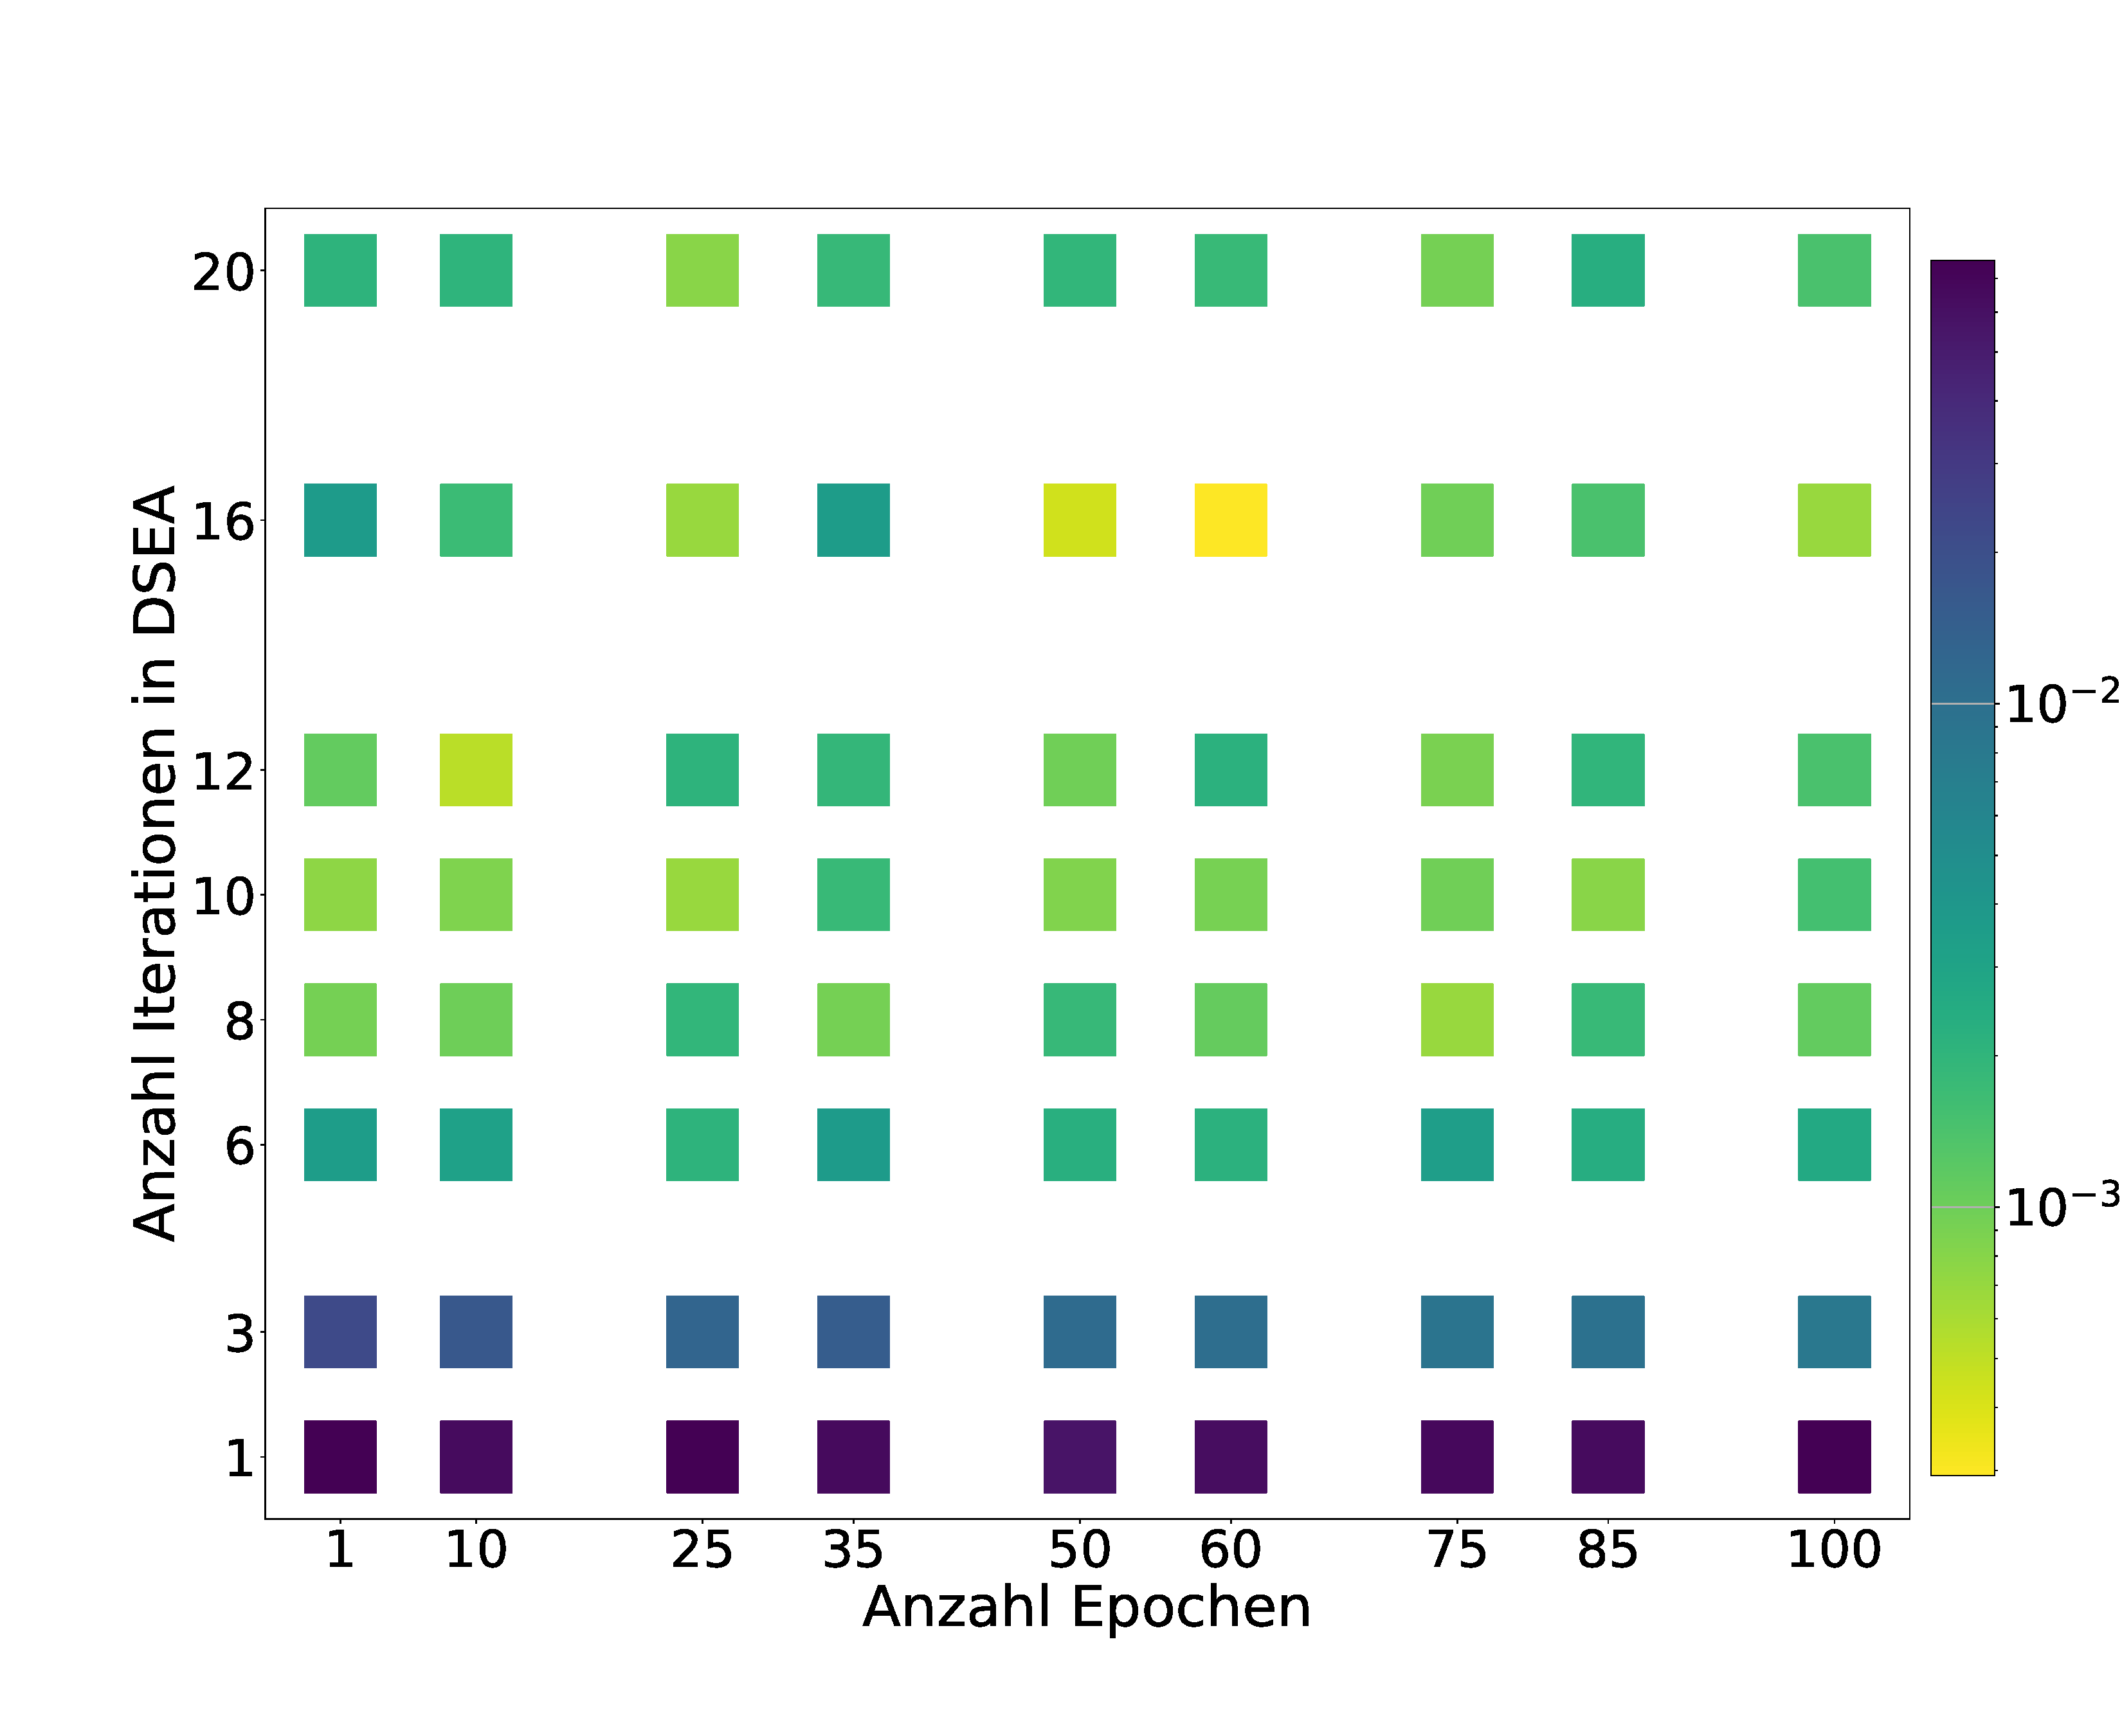
\includegraphics[width=\textwidth]{Plots/DSEA/True/scatter_chi2.pdf}
    \caption[Ergebnisse der Gittersuche für ein NN in DSEA]{Streudiagramm zur Darstellung der Ergebnisse der Gittersuche für \textit{one\_model=True}.
    Der Trainingsprozess des Modells wird in jeder DSEA-Iteration mit angepassten Gewichten fortgesetzt.
    Die logarithmisch-skalierte Farbskala gibt den $\Chi^2$-Abstand zwischen dem wahren und vorhergesagten Spektrum an.
    }
    \label{fig:scatter_true}
\end{figure}

% Trainingsprozess
\subsection{Trainingsprozess} \label{sec:dsea_training}
Der Verlauf des Trainingsprozess des 2. Modells in \autoref{fig:dsea_history_true} hat einen näherungsweisen stetigen Verlauf.
\begin{figure}%
    \begin{subfigure}{0.5\textwidth}%
        \centering%
        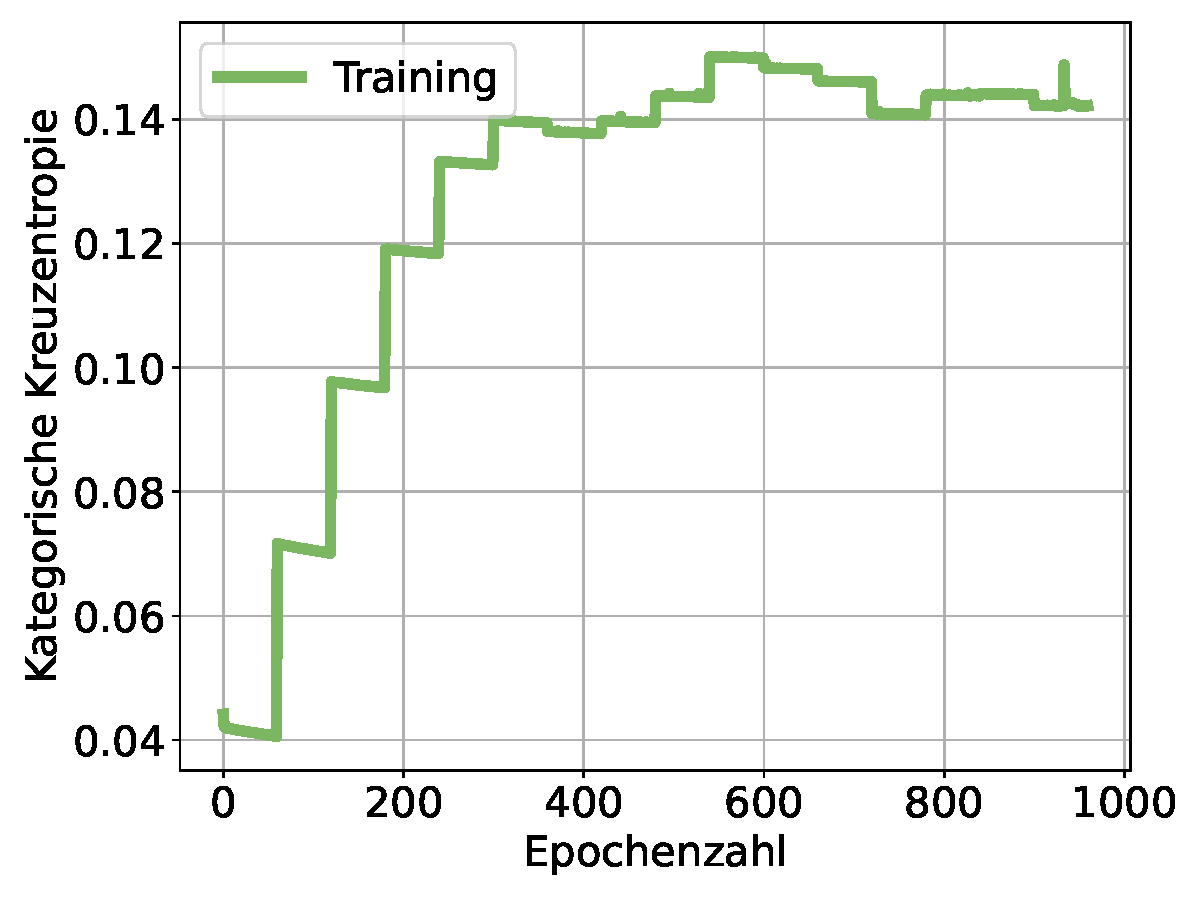
\includegraphics[height=5cm]{Plots/DSEA/True/loss.pdf}%
        \caption{Kostenfunktion: Kategorische Kreuzentropie}%
        %\label{fig:NN_loss}%
    \end{subfigure}%
    \hfill% Fills available space in the center -> space between figures
    \begin{subfigure}{0.5\textwidth}%
        \centering%
        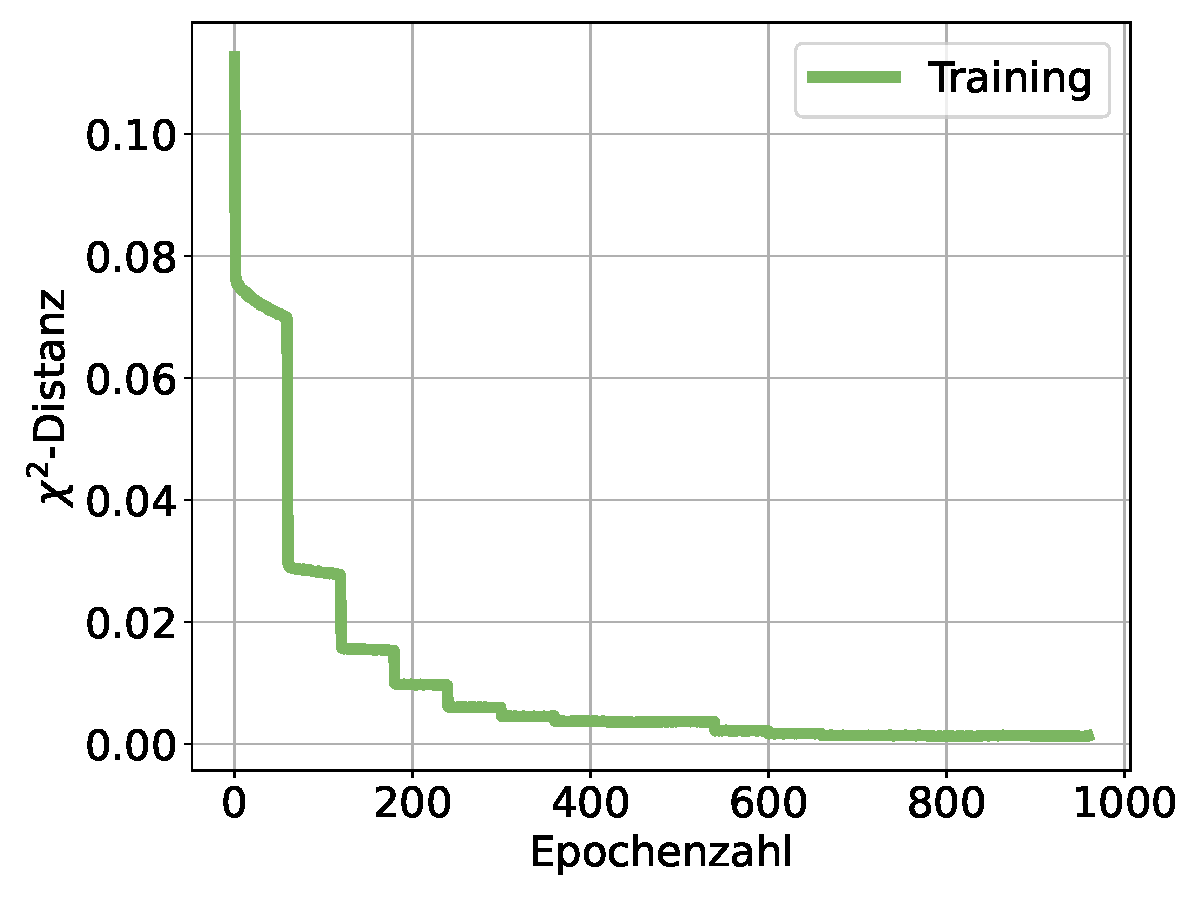
\includegraphics[height=5cm]{Plots/DSEA/True/chi.pdf}%
        \caption{Metrik: $\Chi^2$-Distanz}%
        %\label{fig:NN_chi}%
    \end{subfigure}%
    \caption[Verlauf des Trainingsprozess des 2. Modells in DSEA]{Verlauf des Trainingsprozess des 2. Modells mit dem Parameter \textit{one\_model=True}.
    Im gesamten Trainingsverlauf wird ein Modell trainiert, wobei die Gewichte in jeder DSEA-Iteration angepasst werden.
    Zum einen ist die Kostenfunktion \textit{kategorische Kreuzentropie} und zum anderen die \textit{Chi-Quadrat-Distanz} als Metrik in Abhängigkeit der Epochenzahl aufgeführt.
    }
    \label{fig:dsea_history_true}%
\end{figure}%}
Das liegt daran, dass über den gesamten Prozess nur die Kostenfunktion eines Modells betrachtet wird.
Kleine Unstetigkeiten werden durch die angepassten Gewichte am Ende jeder DSEA-Iteration verursacht.
\\
Anders sieht es bei dem Trainingsverlauf des 1. Modells in \autoref{fig:dsea_history_false} aus.
In jeder DSEA-Iteration wird ein neues Modell erstellt und die Optimierung der Kostenfunktion beginnt von vorne.
Dies ist der Grund für den sprungartigen Verlauf der Metrik und der Verlustfunktion.
\\
Die $\Chi^2$-Distanz beider Modelle sinkt mit der Epochenzahl und konvergiert.
Hingegen steigt die kategorische Kreuzentropie bei jeder Neugewichtung.
Die Gewichte werden in der Kostenfunktion aktualisiert und führen zu einem Anstieg.
Die angepasste Kostenfunktion wird in den darauffolgenden Epochen bis zur nächsten Iteration minimiert.
Sie konvergiert, wenn auch die Gewichte konvergieren.

% Spektrum (Bootstrap in Anhang)
\subsection{Spektrum} \label{sec:dsea_spectrum}
Das entfaltete Spektrum ist für das 2. Modell in \autoref{fig:dsea_spectrum_true} bzw. für das 1. Modell in \autoref{fig:dsea_spectrum_false} abgebildet.
Es treten Oszillationen im gesamten Energiebereich auf.
Diese verstärken sich, insbesondere bei Modell 1 zu höheren Energien.
\\
Auffällig sind auch die ungewöhnlich großen absoluten Abstände in den ersten vier Energie-Bins.
Aufgrund der hohen Statistik in diesen Bins (viele Events im niedrigen Energiebereich) werden hier kleine Abweichungen erwartet.
Eine mögliche Ursache ist, dass die Hochenergie-Bins eine stärkere Gewichtung als die Bins im niederenergetischen Bereich erfahren.
Dadurch werden die Events mit hohen Energien im Trainingsprozess mehr berücksichtigt.
Die Verteilung der Ergebnisse des Bootstrap-Verfahrens zur Bestimmung der Unsicherheiten kann im Anhang eingesehen werden (Modell 1 im Anhang \ref{fig:dsea_bootstrap_true}, Modell 2 im Anhang \ref{fig:dsea_bootstrap_false}).
\begin{figure}
    \centering
    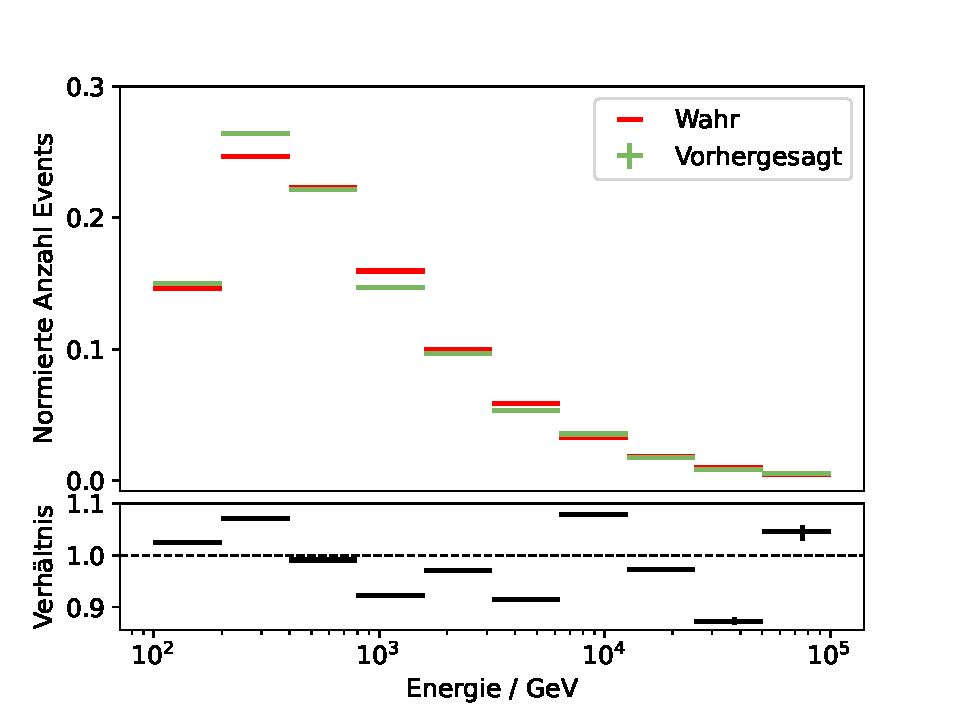
\includegraphics[width=0.9\textwidth]{Plots/DSEA/True/spectrum_dist_10bins_60ep_500000samples_200pulls.pdf}
    \caption[Spektrum des 2. Modells in DSEA]{Das entfaltete Spektrum des 2. Modells mit dem Parameter \textit{one\_model=True}.
    Im gesamten Trainingsverlauf wird ein Modell trainiert, wobei die Gewichte in jeder DSEA-Iteration angepasst werden.
    Der untere Teil zeigt das Verhältnis zwischen wahrem und vorhergesagtem Spektrum und dient als Maß für die relative Abweichung.
    }
    \label{fig:dsea_spectrum_true}
\end{figure}

% Correlation
\subsection{Korrelation} \label{sec:dsea_correlation}
Die Vorhersage einzelner Events (Modell 1 im Anhang \ref{fig:dsea_single_events_false}, Modell 2 im Anhang \ref{fig:dsea_single_events_true}) weisen für beide Modelle nur geringe Unterschiede auf.
Je nach Event variiert die Verteilung der Konfidenzen unterschiedlich stark.
\\
Aufällig sind hier die starken Korrelationen zu den benachbarten Bins.
Dies wird auch durch die Korrelationsmatrix in \autoref{fig:dsea_correlation_true} für Modell 2 (bzw. für Modell 1 im Anhang \ref{fig:dsea_correlation_false}) bestätigt.
\begin{figure}
    \centering
    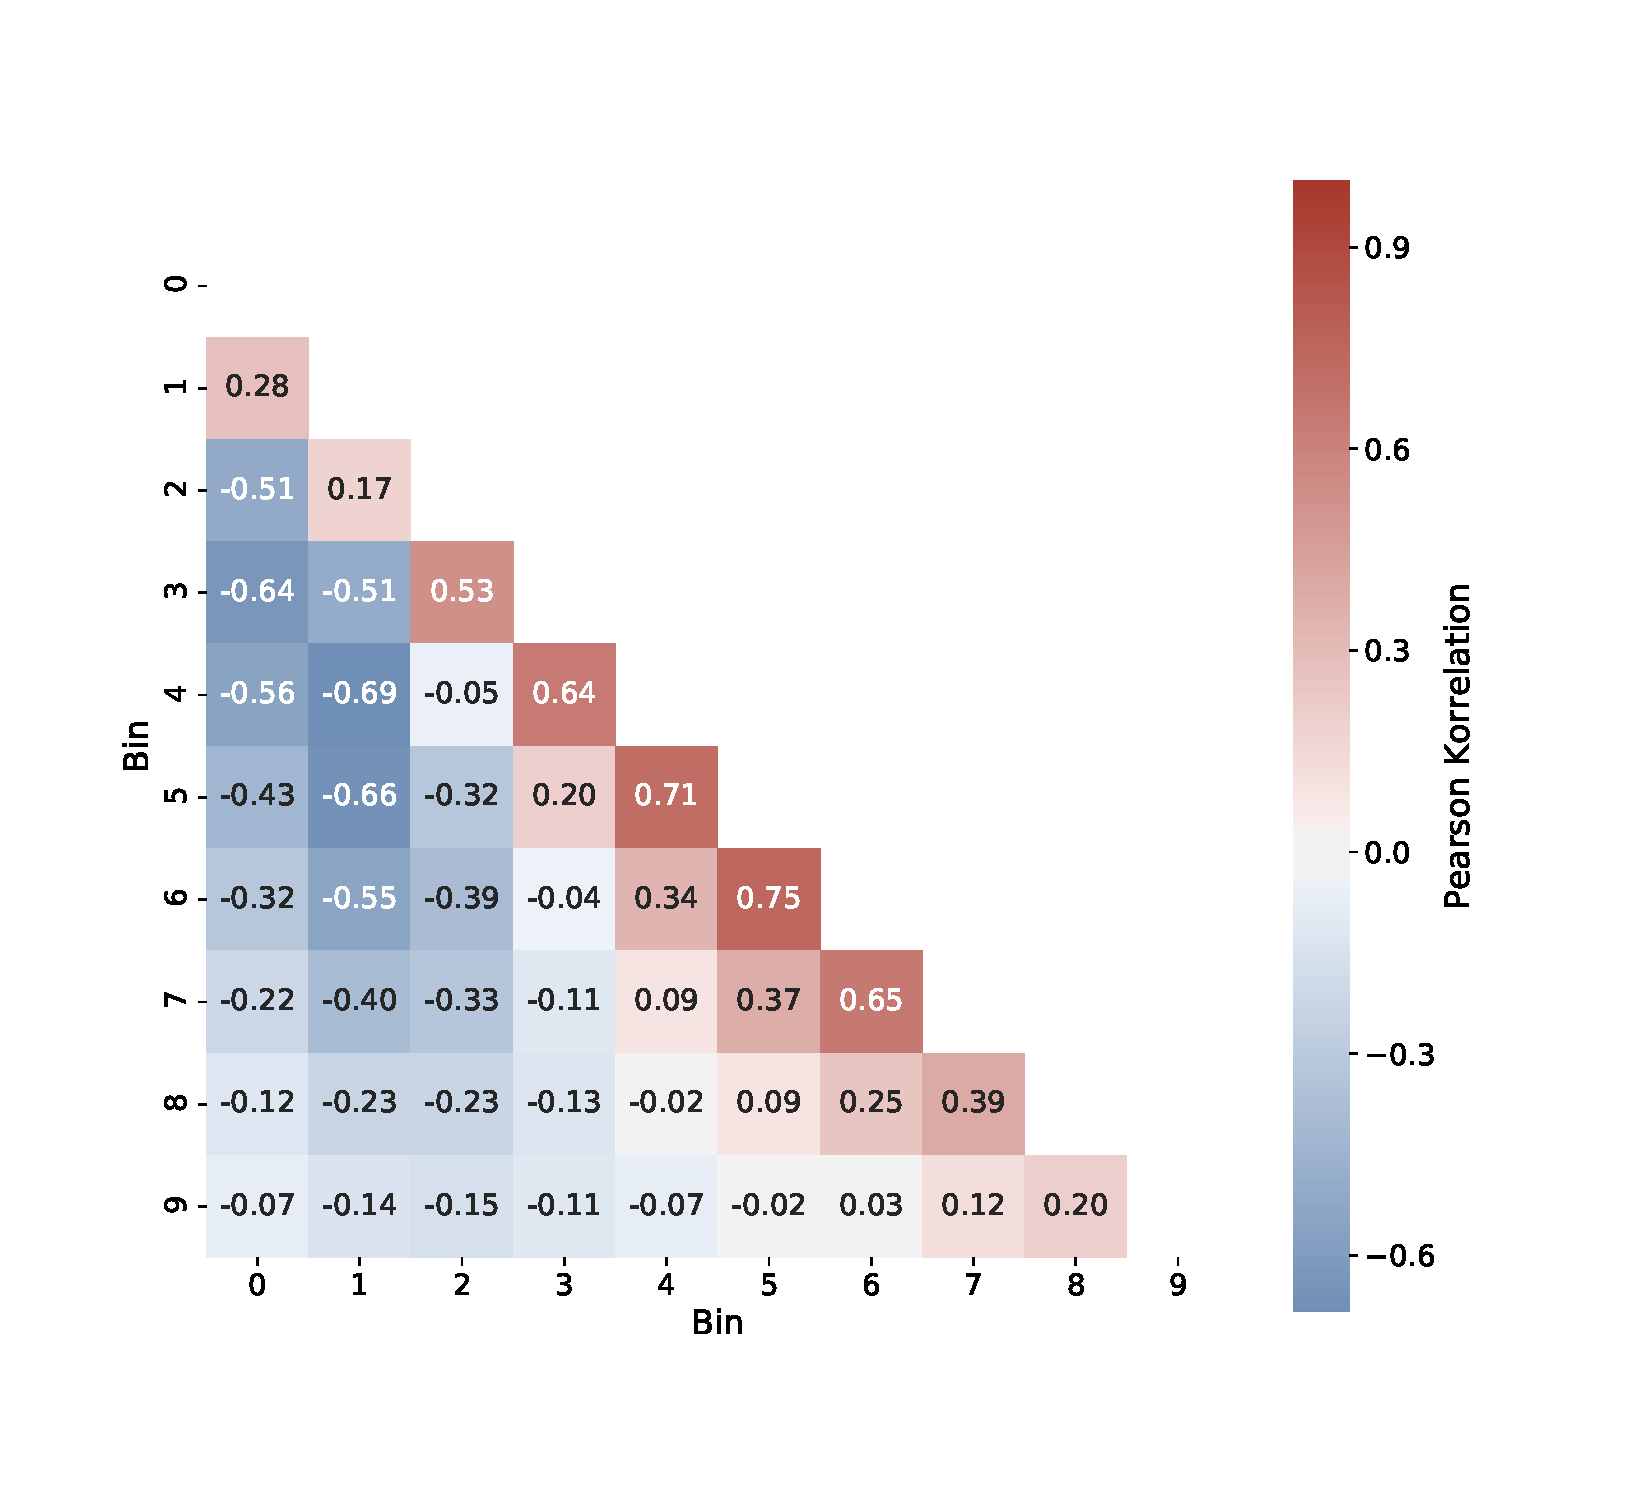
\includegraphics[width=1\textwidth]{Plots/DSEA/True/correlation_matrix.pdf}
    \caption[Korrelationsmatrix des 2. Modells in DSEA]{Die Korrelationsmatrix des 2. Modells (\textit{one\_model=True}).
    Sie gibt die Korrelationen zwischen den entfalteten Energie-Bins an.
    }
    \label{fig:dsea_correlation_true}
\end{figure}
Die benachbarten Bins sind stark positiv korreliert.
Wird also der $n$-te Bin vorhergesagt, so werden dem ($n$-1)-ten und ($n$+1)-ten Bin ebenfalls hohe Konfidenzen zugeordnet.
Die Korrelation nimmt zu entfernten Energien ab.
\\
Im niederenergetischen Bereich treten starke negative Korrelationen auf.
Insbesondere sind die Bins 3-6 mit Bin 1 korreliert.
Dies lässt sich auf die hohe Statistik im Bin 1 zurückführen.
Diesem Energiebereich sind die meisten Events zuzuordnen.
Wird nun exemplarisch der 4. Bin vorhergesagt, so wird dem 1. Bin eine niedrigere Konfidenz als im Durchschnitt zugeordnet.
% BIAS
\section{Abhängigkeit der Entfaltung vom Trainingsspektrum} \label{sec:bias}
In diesem Kapitel wird die Abhängigkeit des entfalteten Spektrums von den Trainingsdaten (\textit{Bias}) untersucht.
Dazu wird aus dem bekannten MC-Datensatz eine Teilprobe mit gleichverteilten Klassen erstellt.
Die Methode wird als \textit{Undersampling} bezeichnet.
\\
Die Probe beinhaltet von jeder der 10 Energie-Klassen \SI{50000}{\text{Events}} und umfasst somit insgesamt \SI{500000}{\text{Events}}.
Diese Teilprobe wird als Trainingsdatensatz verwendet.
Entfaltet und evaluiert werden \SI{500000}{\text{Events}} des bekannten Neutrino-Spektrums.
\\
Zum einen wird der Bias des gleichen NN, wie in \autoref{sec:nn_no_dsea} untersucht.
Zum anderen wird die Entfaltung eines NN in DSEA auf eine Abhängigkeit geprüft.
%Die Parameter des 1. Modells (siehe \autoref{sec:deconv_dsea}) sollen dabei verwendet werden.
% NN
\\
In \autoref{fig:bias_nn} sind die Ergebnisse des auf \SI{50}{\text{Epochen}} trainierten NN dargestellt.
\begin{figure}
    \centering
    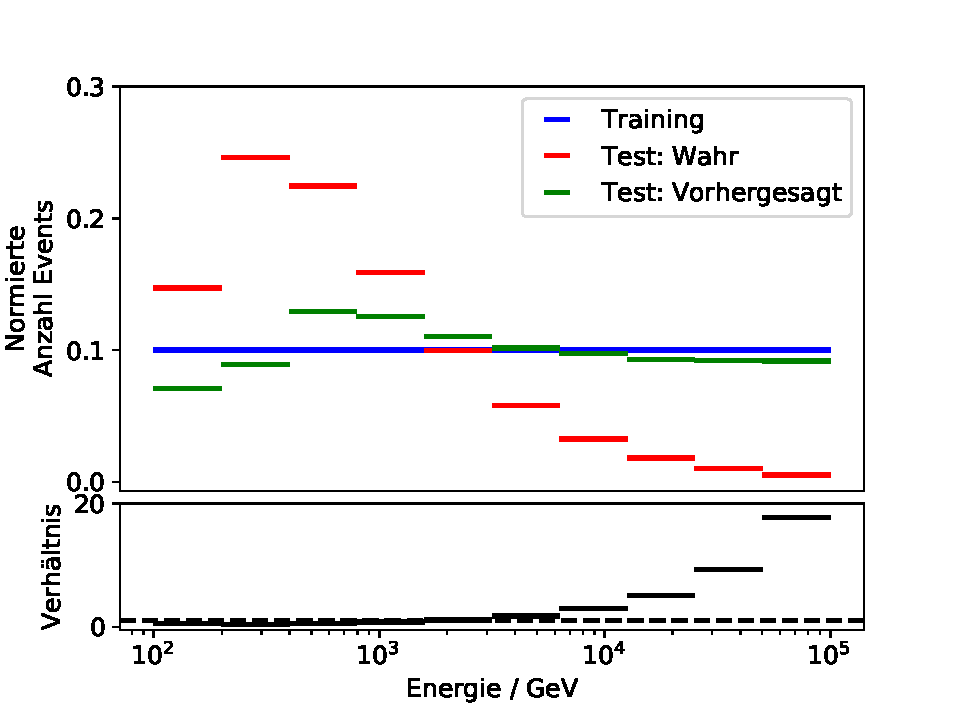
\includegraphics[width=0.9\textwidth]{Plots/BIAS/NN/spectrum.pdf}
    \caption[Überprüfung des Bias: Spektrum des NN ohne DSEA]{Das mit einem NN entfaltete Energiespektrum, der Neutrinos bei Verwendung von Trainingsdaten mit gleichverteilten Klassen.
    Vergleich der Spektren der Trainingsdaten (Blau), der wahren Evaluationsdaten (Rot) und der entfalteten Evaluationsdaten (Grün).
    }
    \label{fig:bias_nn}
\end{figure}
Zu sehen ist das Spektrum der gleichverteilten Trainingsdaten in Blau, der entfalteten Daten in Grün und des wahren Spektrums in Rot.
Das vorhergesagte Spektrum liegt nahe dem Trainingsspektrum.
Nur in Bin 3 und 4 wird das Maximum des zu entfaltenden Spektrums leicht angedeutet.
Insgesamt ist also ein starker Bias zu beobachten.
% DSEA
\\
Im folgenden wird das 1. Modell (\SI{12}{\text{Iterationen}}, \SI{75}{\text{Epochen}}, \textit{one\_model=False}) zur Entfaltung des Neutrino-Spektrums verwendet.
Trainiert wird das Modell auf den gleichverteilten Daten.
Die Spektren sind analog zum vorherigen Plot in \autoref{fig:bias_dsea_false} graphisch dargestellt.
Das entfaltete Spektrum unterscheidet sich erheblich von den Trainingsdaten.
Im Hochenergiebereich werden die Bins stark überschätzt.
Auch die anderen entfalteten Energiebereiche passen nur bedingt mit dem wahren Spektrum überein.
Dies liegt hier nicht an einer starken Abhängigkeit von den Daten, sondern lässt sich auf die geringe Accuracy zurückführen.
\\
Der gleiche Prozess wird für das 2. Modell (\SI{16}{\text{Iterationen}}, \SI{60}{\text{Epochen}}, \textit{one\_model=True}) durchgeführt.
Das entfaltete Spektrum in \autoref{fig:bias_dsea_true} weist starke Abweichungen von der wahren Verteilung auf.
Insbesondere die Hochenergie-Bins werden überschätzt.
Insgesamt unterscheiden sich die entfalteten Verteilungen signifikant von dem Trainingsspektrum.
Die Modellunabhängigkeit von DSEA wird dadurch wiedermal bestätigt.
\begin{figure}
    \centering
    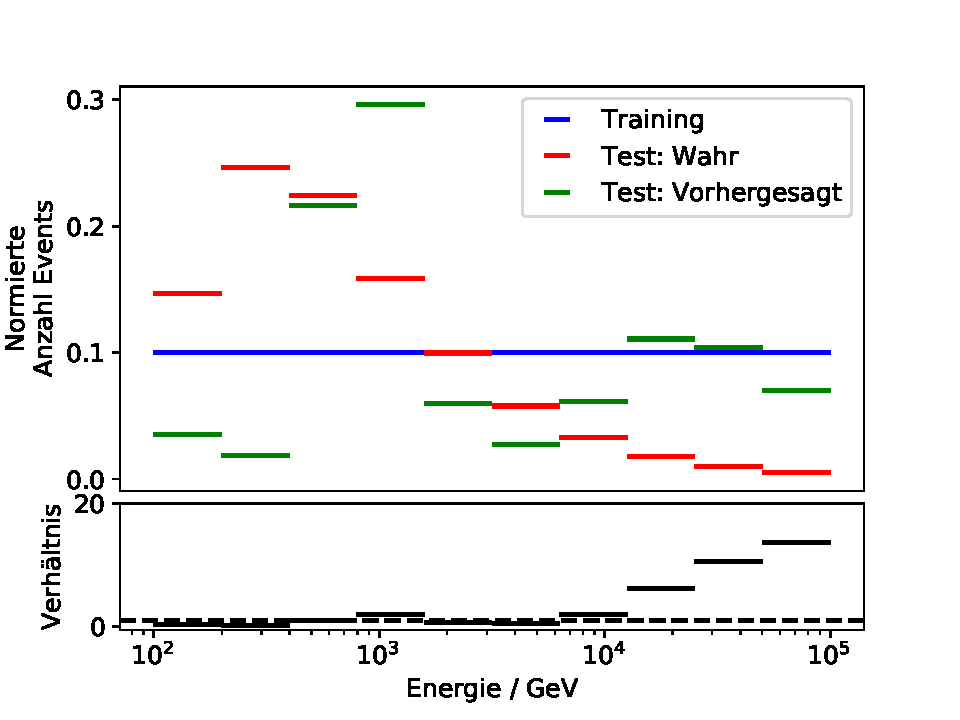
\includegraphics[width=0.9\textwidth]{Plots/BIAS/DSEA/spectrum_12it_75ep_False.pdf}
    \caption[Überprüfung des Bias: Spektrum des 1. Modells in DSEA]{Das mit einem NN in DSEA entfaltete Energiespektrum der Neutrinos.
    Das NN (Modell 1) wird in DSEA auf einem Datensatz mit gleichverteilten Klassen trainiert.
    Dargestellt ist das Spektrum der Trainingsdaten (Blau), der wahren Evaluationsdaten (Rot) und der entfalteten Evaluationsdaten (Grün).
    }
    \label{fig:bias_dsea_false}
\end{figure}

\chapter{Fazit und Ausblick}

%Ziel der Arbeit und zusammenfassung
Ziel der Arbeit ist die Untersuchung von Entfaltungen mit neuronalen Netzen in \textbf{DSEA}.
Das Verhalten der Parameter \textit{Epochenzahl} und Anzahl \textit{DSEA-Iterationen} wurde systematisch untersucht.
Es wurde geprüft, wie sich NN in DSEA entwickeln, wenn in jeder Iteration ein neues Modell erstellt und trainiert wird.
Ebenfalls wurde eine neue Methode geprüft, die nur bei auf Verlustfunktion basierenden Klassifizierern möglich ist.
Statt in jeder Iteration ein neues Modell zu erstellen, werden die Gewichte der Kostenfunktion \textbf{eines} Modells angepasst.
Dies führt zu einer schnelleren Konvergenz.
Ein signifkanter Unterschied im resultierenden Spektrum konnte jedoch nicht festgestellt werden.
\\
%Vergleich NN und NN in DSEA: modellunabhängig, geringerer bias,
Ebenfalls wurde eine Entfaltung über eine klassische Klassfikation mit einem NN betrachtet.
Die Abhängigkeit vom Trainingsspektrum dieses Modells und der von neuronalen Netze in DSEA wurde zuletzt geprüft.
Die Entfaltung über eine klassische Klassifikation zeigt einen starken Bias.
NN in DSEA weisen auch eine große Abweichung vom wahren Spektrum auf.
In diesem Fall liegt das nicht an einem Bias, sondern an der geringen Accuracy $< \SI{39}{\percent}$.
Die Modellunabhängigkeit von DSEA konnte hier bestätigt werden.
\\
%Datensatz mit gewählten features war schwierig zu entfalten.
Allgemein weisen die Entfaltungen des vorliegenden Datensatzes große Abweichungen auf.
Die Entfaltung mit NN in DSEA kann möglicherweise durch einen Datensatz der Rohdaten beinhaltet verbessert werden.
Grund dafür ist, dass die Stärke von NN nicht in der Klassifikation von tabellarischen Daten liegt.
Bei der Klassifikation von graphischen Daten sind Convolutional Neural Networks ("`Faltendes Neuronales Netzwerk"'), kurz \textbf{CNN} unersetzbar.
Optimal ist dafür ein Datensatz, der die drei-dimensionale Struktur des Detektors widerspiegelt.
Dies zeigt auch die Arbeit \cite{reconstruction_nn} über die Rekonstruktion von Neutrinoereignissen mit graphischen neuronalen Netzen (GNN), die eine Erweiterung der CNNs \cite{reconstruction_nn} darstellen.
\\
% weitere NN mit mehr parameter testen mit Regularisierung
Größere Modelle mit mehr Parameter haben grundsätzlich ein größeres Potenzial.
Um Overfitting zu reduzieren, können Methoden der Regularisierung, wie die L2-Parameter-Regularisierung, Dropout oder die Batch-Norm verwendet werden.
\\
Auffällig waren die in allen Entfaltungen auftretenden Oszillationen.
Zur Glättung dieser Störung könnte ebenfalls ein Regularisierungsterm in der Kostenfunktion beitragen.
Analog zur Tikhonov-Regularisierung\cite{tikhonov}, könnte Glattheit über eine kleine zweite Ableitung gefordert werden.

\appendix
% Hier beginnt der Anhang, nummeriert in lateinischen Buchstaben
\chapter{Monte-Carlo Sample}
    
%\begin{tabular}{ l }
    %\centering
    %\caption{Eine Tabelle mit Messdaten.}
    %\label{tab:features}
    %\hline
    %Featurename \\
    %\hline
    %SplineMPEDirectHitsICE.n_dir_doms \\ 
    %VariousVariables.Cone_Angle \\
    %SplineMPECramerRaoParams.variance_theta \\
    %Borderness.Q_ratio_in_border \\
    %SplineMPETruncatedEnergy_SPICEMie_BINS_MuEres.value \\
    %SplineMPETruncatedEnergy_SPICEMie_DOMS_Neutrino.energy \\
    %SplineMPEDirectHitsICB.n_late_doms \\
    %Dustyness.n_doms_in_dust \\
    %LineFitGeoSplit1Params.n_hits \\
    %SplineMPEDirectHitsICC.dir_track_hit_distribution_smoothness \\
    %SPEFit2GeoSplit1BayesianFitParams.logl \\
    %SplineMPECharacteristicsIC.avg_dom_dist_q_tot_dom \\
%\end{tabular}
\begin{table}
    \centering
    \caption{Namen der verwendeten Features aus dem Monte-Carlo 11374 Datensatz.}
    \label{tab:feature}
    \begin{tabular}{l}
        \toprule
        Featurename \\
        \midrule
        SplineMPEDirectHitsICE.n\_dir\_doms \\
        VariousVariables.Cone\_Angle \\
        SplineMPECramerRaoParams.variance\_theta \\
        Borderness.Q\_ratio\_in\_border \\
        SplineMPETruncatedEnergy\_SPICEMie\_BINS\_MuEres.value \\
        SplineMPETruncatedEnergy\_SPICEMie\_DOMS\_Neutrino.energy \\
        SplineMPEDirectHitsICB.n\_late\_doms \\
        Dustyness.n\_doms\_in\_dust \\
        LineFitGeoSplit1Params.n\_hits \\
        SplineMPEDirectHitsICC.dir\_track\_hit\_distribution\_smoothness \\
        SPEFit2GeoSplit1BayesianFitParams.logl \\
        SplineMPECharacteristicsIC.avg\_dom\_dist\_q\_tot\_dom \\
        \bottomrule
    \end{tabular}
\end{table}
\chapter{Entfaltung als Klassifikationsproblem}
\begin{table}
    \centering
    \begin{tabular}{l l l l}
        \toprule
        Ebene & Aktivierungsfunktion & Eingangsdimension & Ausgangsdimension \\
        \midrule
        Eingang & - & $12$ & $12$ \\
        Tief & ReLU & $12$ & $120$ \\
        Tief & ReLU & $120$ & $240$ \\
        Tief & ReLU & $240$ & $120$ \\
        Tief & ReLU & $120$ & $12$ \\
        Ausgang & Softmax & $12$ & $10$ \\
        \bottomrule
    \end{tabular}
    \caption{Die Struktur des neuronalen Netzes von oben nach unten gelesen.
    Die Aktivierungsfunktion und Eingangs- und Ausgangsdimensionen sind für jede Ebene aufgeführt.
    }
    \label{tab:nn_shape}
\end{table}

\begin{table}
    \centering
    \begin{tabular}{l l}
        \toprule
        Parameter & Wert \\
        \midrule
        Epochenzahl & $50$ \\
        Batchgröße & $2048$ \\
        Lernrate (ADAM) & $0.0005$ \\
        \bottomrule
    \end{tabular}
    \caption{Hyperparameter des neuronalen Netzes.}
    \label{tab:nn_params}
\end{table}

\begin{figure}%
    \centering%
    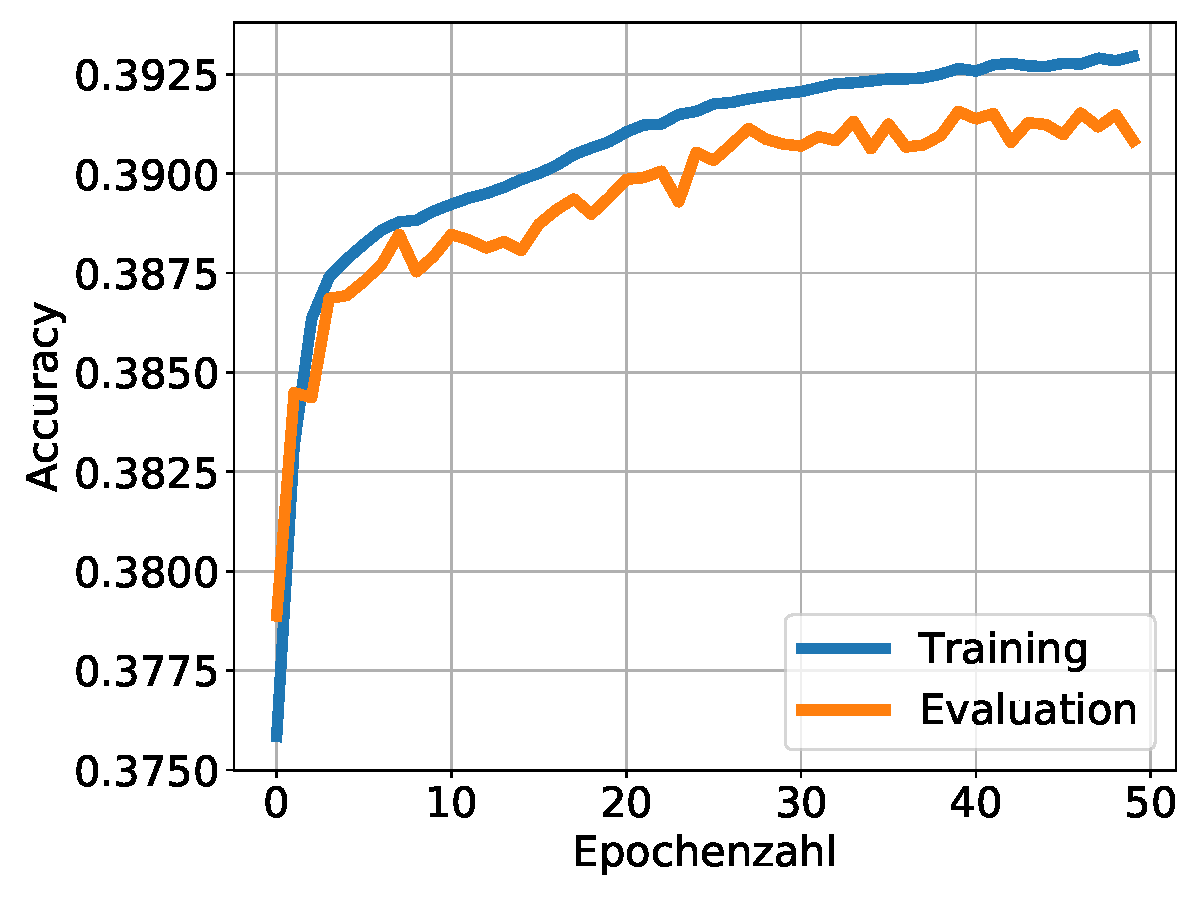
\includegraphics[width=0.7\textwidth]{Plots/NN/acc.pdf}%
    \caption[Verlauf der Accuracy für den Trainingsprozess des NN ohne DSEA]{Verlauf der Accuracy in Abhängigkeit der Epochenzahl für den Trainingsprozess des NN.}%
    \label{fig:NN_acc}%
\end{figure}%

\begin{figure}%
    \centering%
    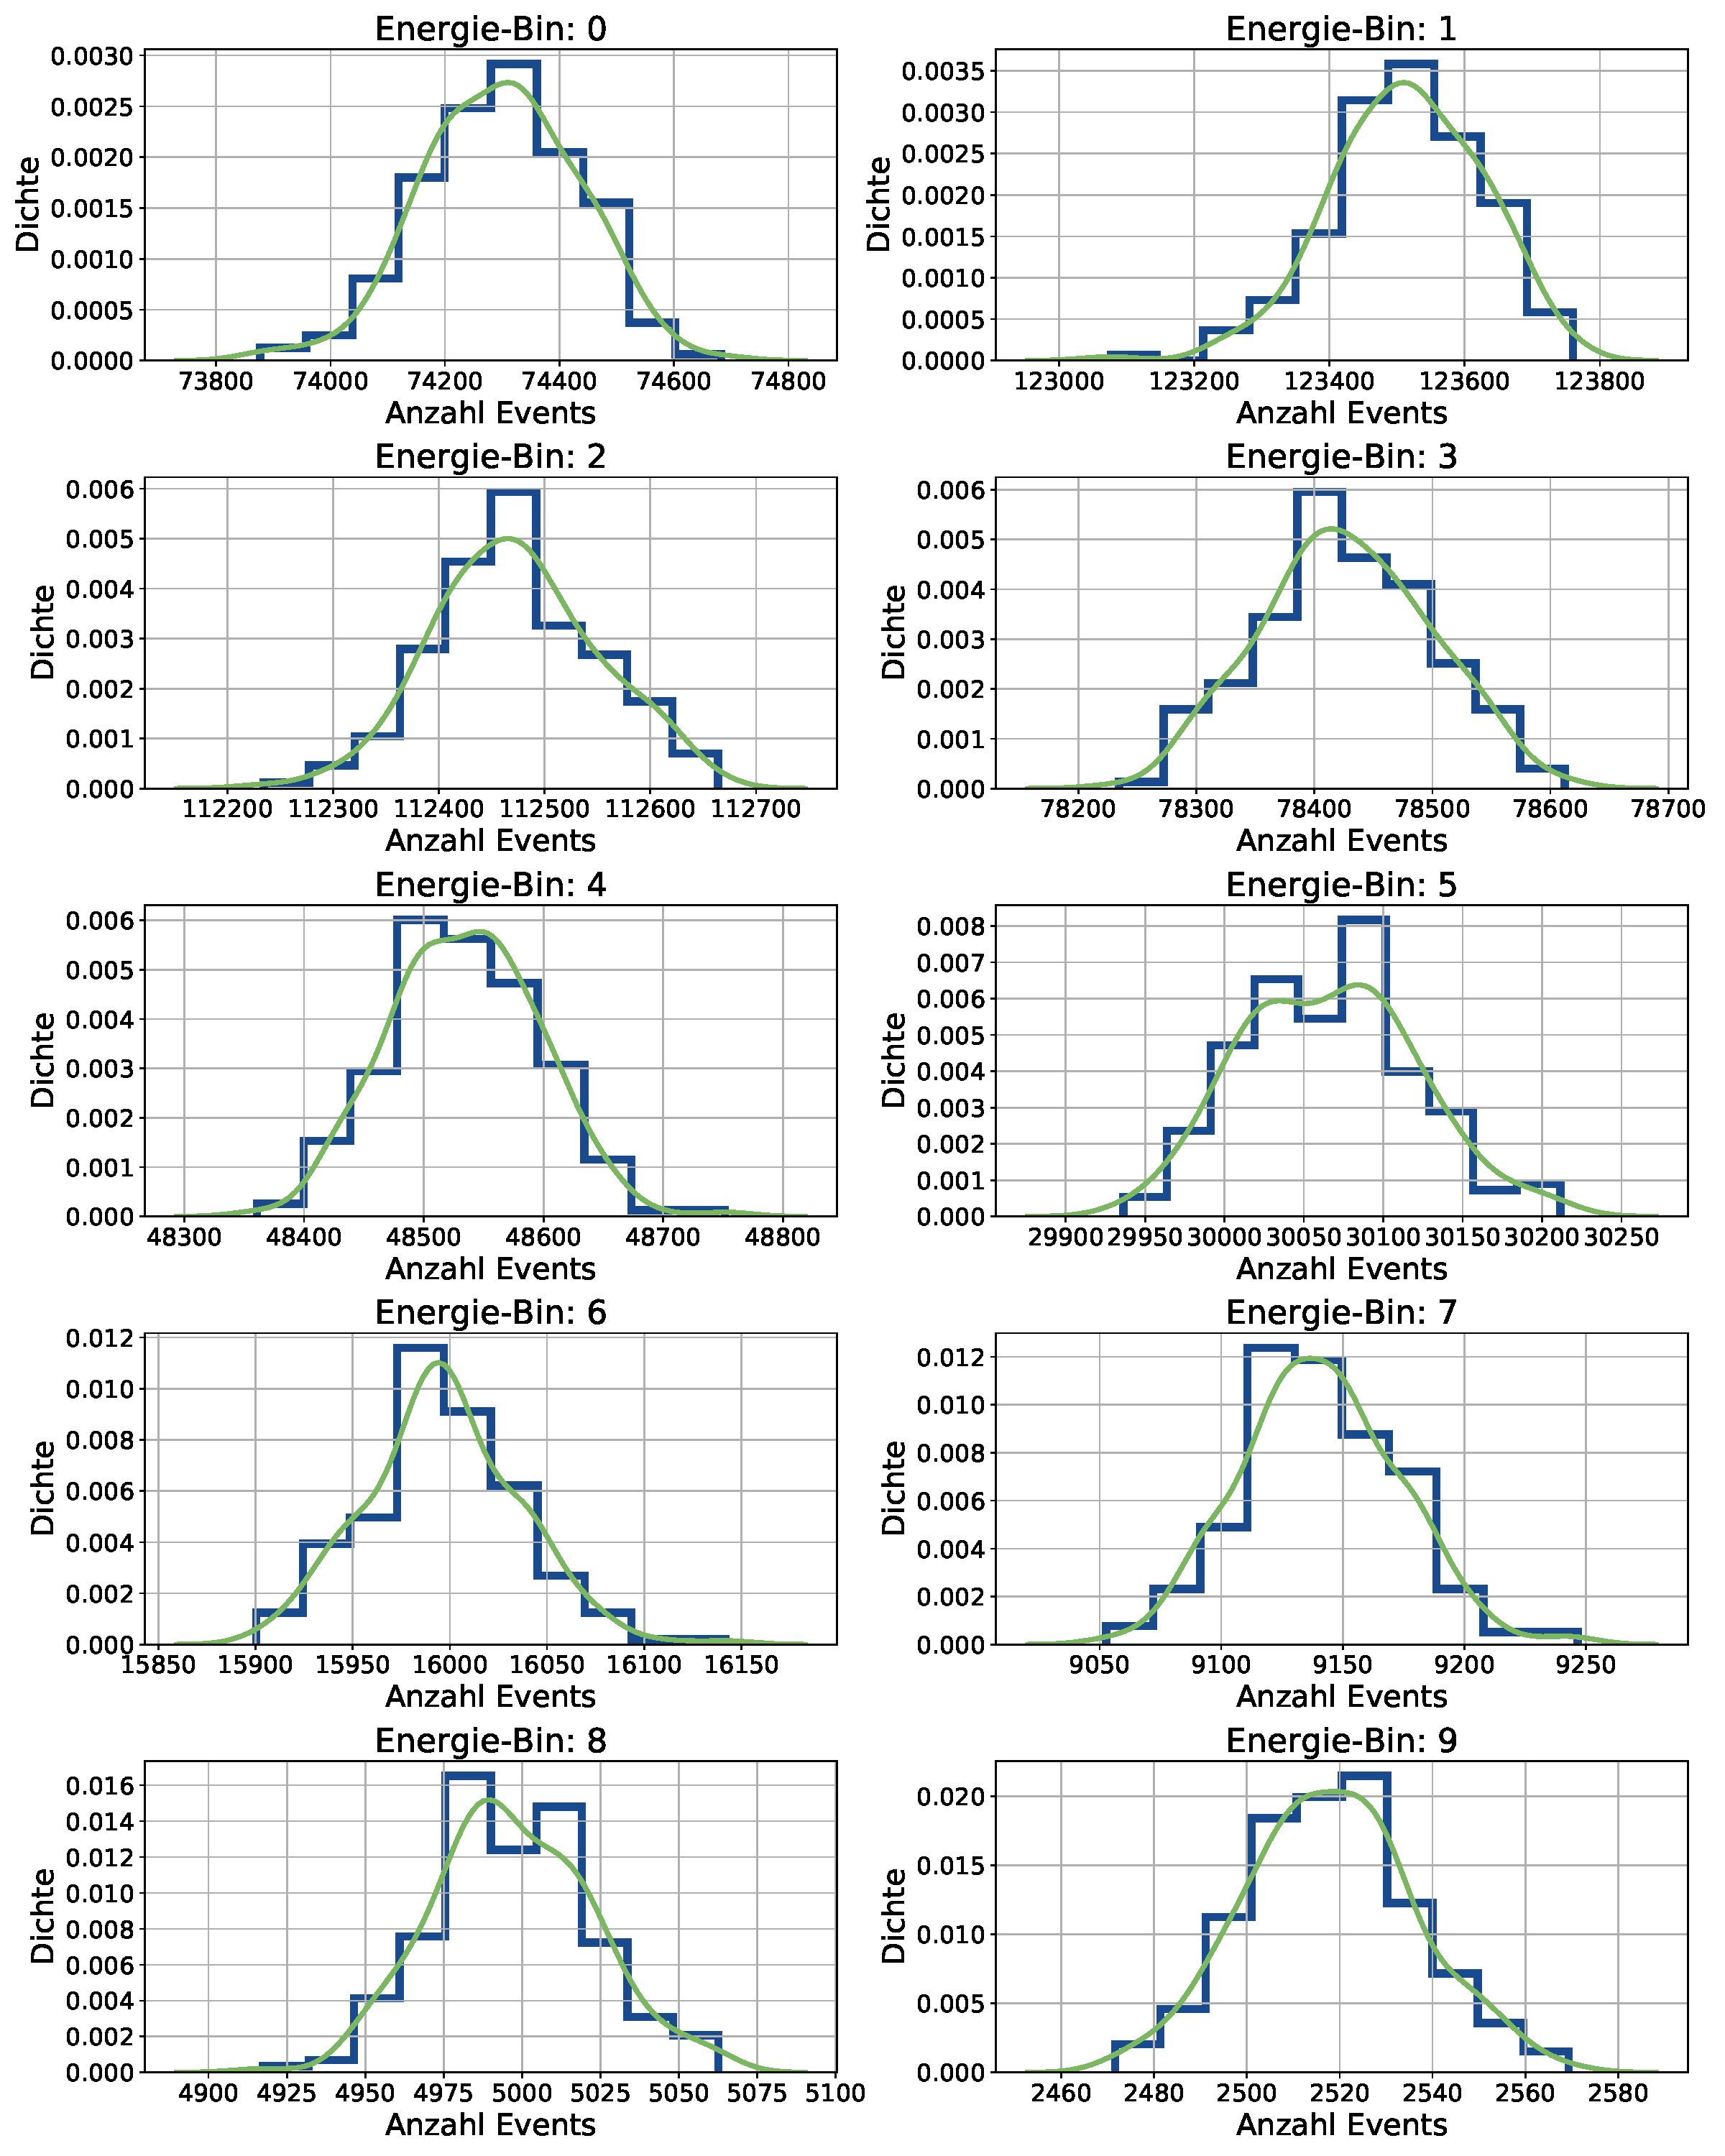
\includegraphics[width=\textwidth]{Plots/NN/class_dist_10bins_50ep_500000samples_200pulls.pdf}%
    \caption[Ergebnisse des Bootstrapping-Vefahrens für das NN ohne DSEA]{Das blaue Histrogramm stellt die Verteilung der Bootstrap-Ergebnisse mit 200 Iterationen dar.
    Die rote Funktion repräsentiert einen Kerndichteschätzer(KDE) mit Gaußkern.
    Die Bin-Höhe wird durch den Median angegeben.
    Über das untere und obere Quantil werden die Unsicherheiten bestimmt.
    }%
    \label{fig:NN_bootstrap}%
\end{figure}%

\begin{figure}%
    \centering%
    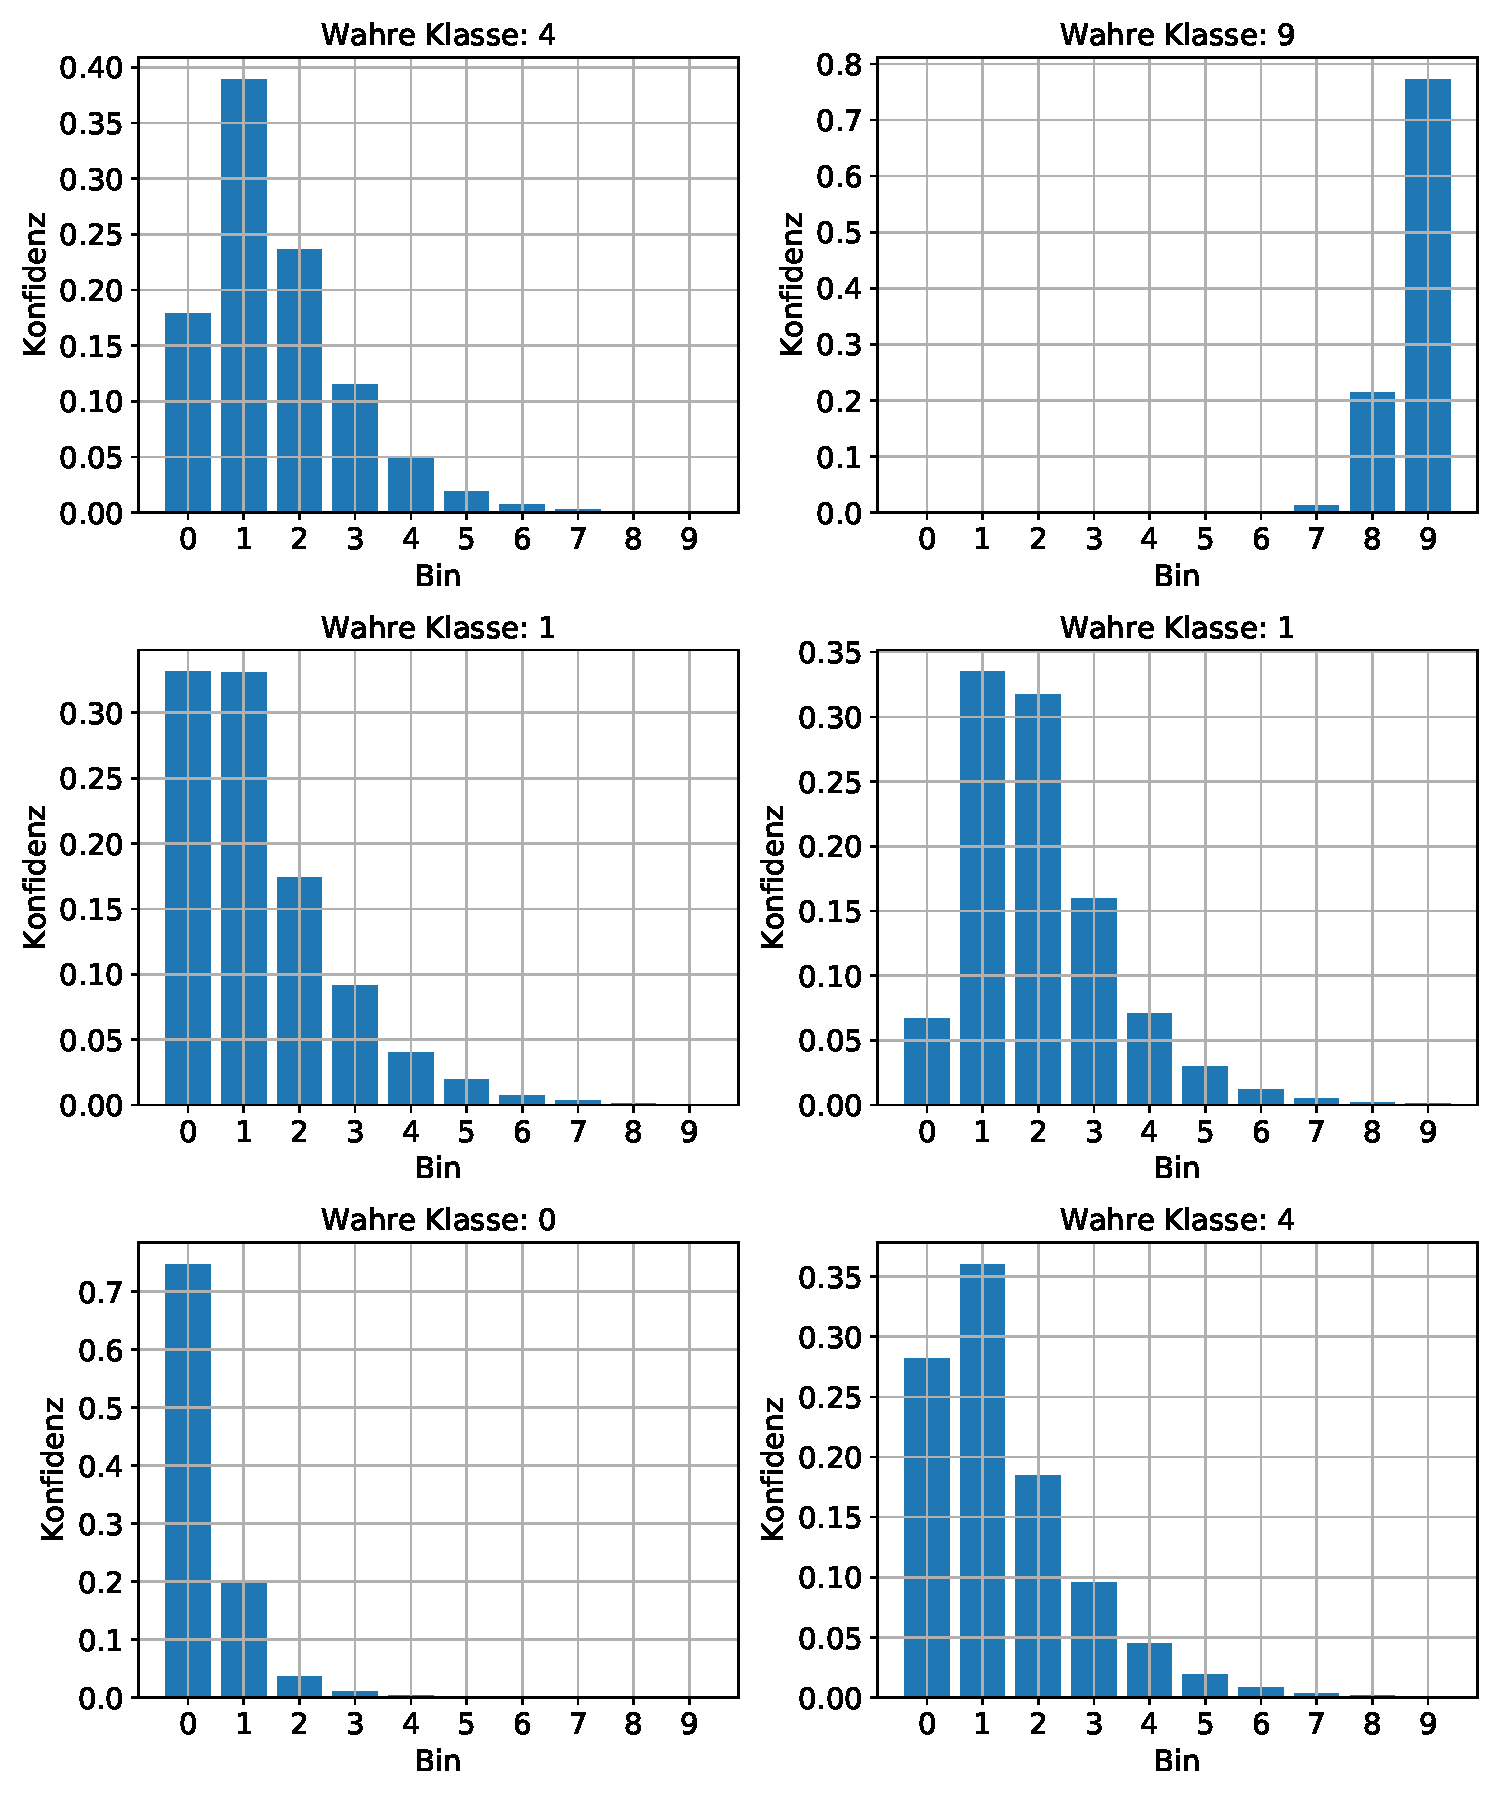
\includegraphics[width=\textwidth]{Plots/NN/single_events.pdf}%
    \caption[Vorhersage einzelner Events des NN ohne DSEA]{Vorhersage einzelner Events des NN.
    Jedem Energie-Bin wird eine Konfidenz zugeordnet.
    Diese gibt die Wahrscheinlichkeit an, dass das betrachtete Event zu dem Energie-Bin gehört.
    }%
    \label{fig:NN_single_events}%
\end{figure}%


\chapter{Entfaltung mit DSEA}

% MAKE MODEL
\begin{lstlisting}[language=Python, basicstyle=\small, captionpos=b, caption=Die Funktion wird zu Erstellung des Modells verwendet. Hier wird das NN mithilfe der Keras-API \cite{tensorflow2015-whitepaper} definiert. Die Ebenen können beliebig angepasst und erweitert werden., label=code:model]
def make_model(num_features, num_classes, learning_rate=0.0005): 
    """
    num_features: Number of features
    num_classes: Number of energy classes
    learning_rate: Hyperparameter of the ADAM optimizer
    """
    model = tf.keras.Sequential()

    # input layer
    model.add(tf.keras.layers.Dense(120, input_shape=num_features,
    activation='relu'))
    
    # dense layer
    model.add(tf.keras.layers.Dense(240, activation='relu'))
    model.add(tf.keras.layers.Dense(120, activation='relu'))
    model.add(tf.keras.layers.Dense(12, activation='relu'))
    
    # output layer
    model.add(tf.keras.layers.Dense(num_classes, activation='softmax'))

    # define optimizer, loss function and metric
    opt = tf.keras.optimizers.Adam(learning_rate=learning_rate)
    loss = tf.keras.losses.CategoricalCrossentropy()
    acc = tf.keras.metrics.CategoricalAccuracy(
        name="categorical_accuracy", dtype=None)

    # compile the tensorflow model
    model.compile(optimizer=opt, loss=loss, metrics=[acc, chi2])

    return model
\end{lstlisting}

\newpage
% WRAPPER
\begin{lstlisting}[language=Python, basicstyle=\small, captionpos=b, caption=Quellcode des Wrappers zur Verwendung der Keras-API\cite{tensorflow2015-whitepaper} in DSEA. Es wird die Funktion \textbf{make\_model} im Anhang \ref{code:model} zur Erstellung der Tensorflow-Modelle benötigt., label=code:wrapper]
class MyClassifier():
    """
    Parameters
    ---------
    one_model: bool
        If True, dsea will train only one model instead of 
        generating a new one in each dsea iteration
    batch_size: int
        Split data into batches with the size of batch_size
    epochs: int
        Number of epochs
    learning_rate: float
        Stepsize of the optimizer ADAM
    """

    def __init__(self, batch_size=2048, epochs=5, learning_rate=0.0005,
    one_model=True):        
        self.batch_size = batch_size
        self.epochs = epochs
        self.learning_rate = learning_rate
        self.one_model = one_model
        self.model = None #tensorflow model if created
        self.Niter = 0 #current DSEA iteration
        self.history = [] #model history for each dsea iteration

    def fit(self, X, y, sample_weight=None):
        # train self.model on weighted data X with label y

        # print progress
        self.Niter += 1
        print(f'\nNumber iteration in DSEA: {self.Niter}')

        # y is NOT one-hot encoded yet
        y_hot = np.zeros((y.size, y.max()+1))
        y_hot[np.arange(y.size),y] = 1
        
        # create new model if (one_model=False) or
        # (one_model = True and there exist no model yet)
        if self.model is None or self.one_model is False:
            self.model = make_model(num_features=(len(feature_list), ),
            num_classes=y.max()+1, learning_rate=self.learning_rate)

        # save training history
        history = self.model.fit(X, y_hot, sample_weight=sample_weight,
        batch_size=self.batch_size, epochs=self.epochs)
        self.history.append(history)

        return self

    def predict_proba(self, X):
        # predict X, returns confidences c_ij for each row i and class j
        return self.model.predict(X)

    def get_model(self):
        # return the tensorflow model
        return self.model

    def get_model_history(self):
        # return the history of loss, accuracy and chi2 distance
        # of the training process
        list_loss = []
        list_acc = []
        list_chi = []

        # list of lists --> one list
        for history in self.history:
            list_loss += history.history['loss']
            list_acc += history.history['categorical_accuracy']
            list_chi += history.history['chi2']

        # list to numpy array
        list_loss = np.array(list_loss, dtype='float32')
        list_acc = np.array(list_acc, dtype='float32')
        list_chi = np.array(list_chi, dtype='float32')

        return list_loss, list_acc, list_chi
\end{lstlisting}

% chi2 scatter: False
\begin{figure}
    \centering
    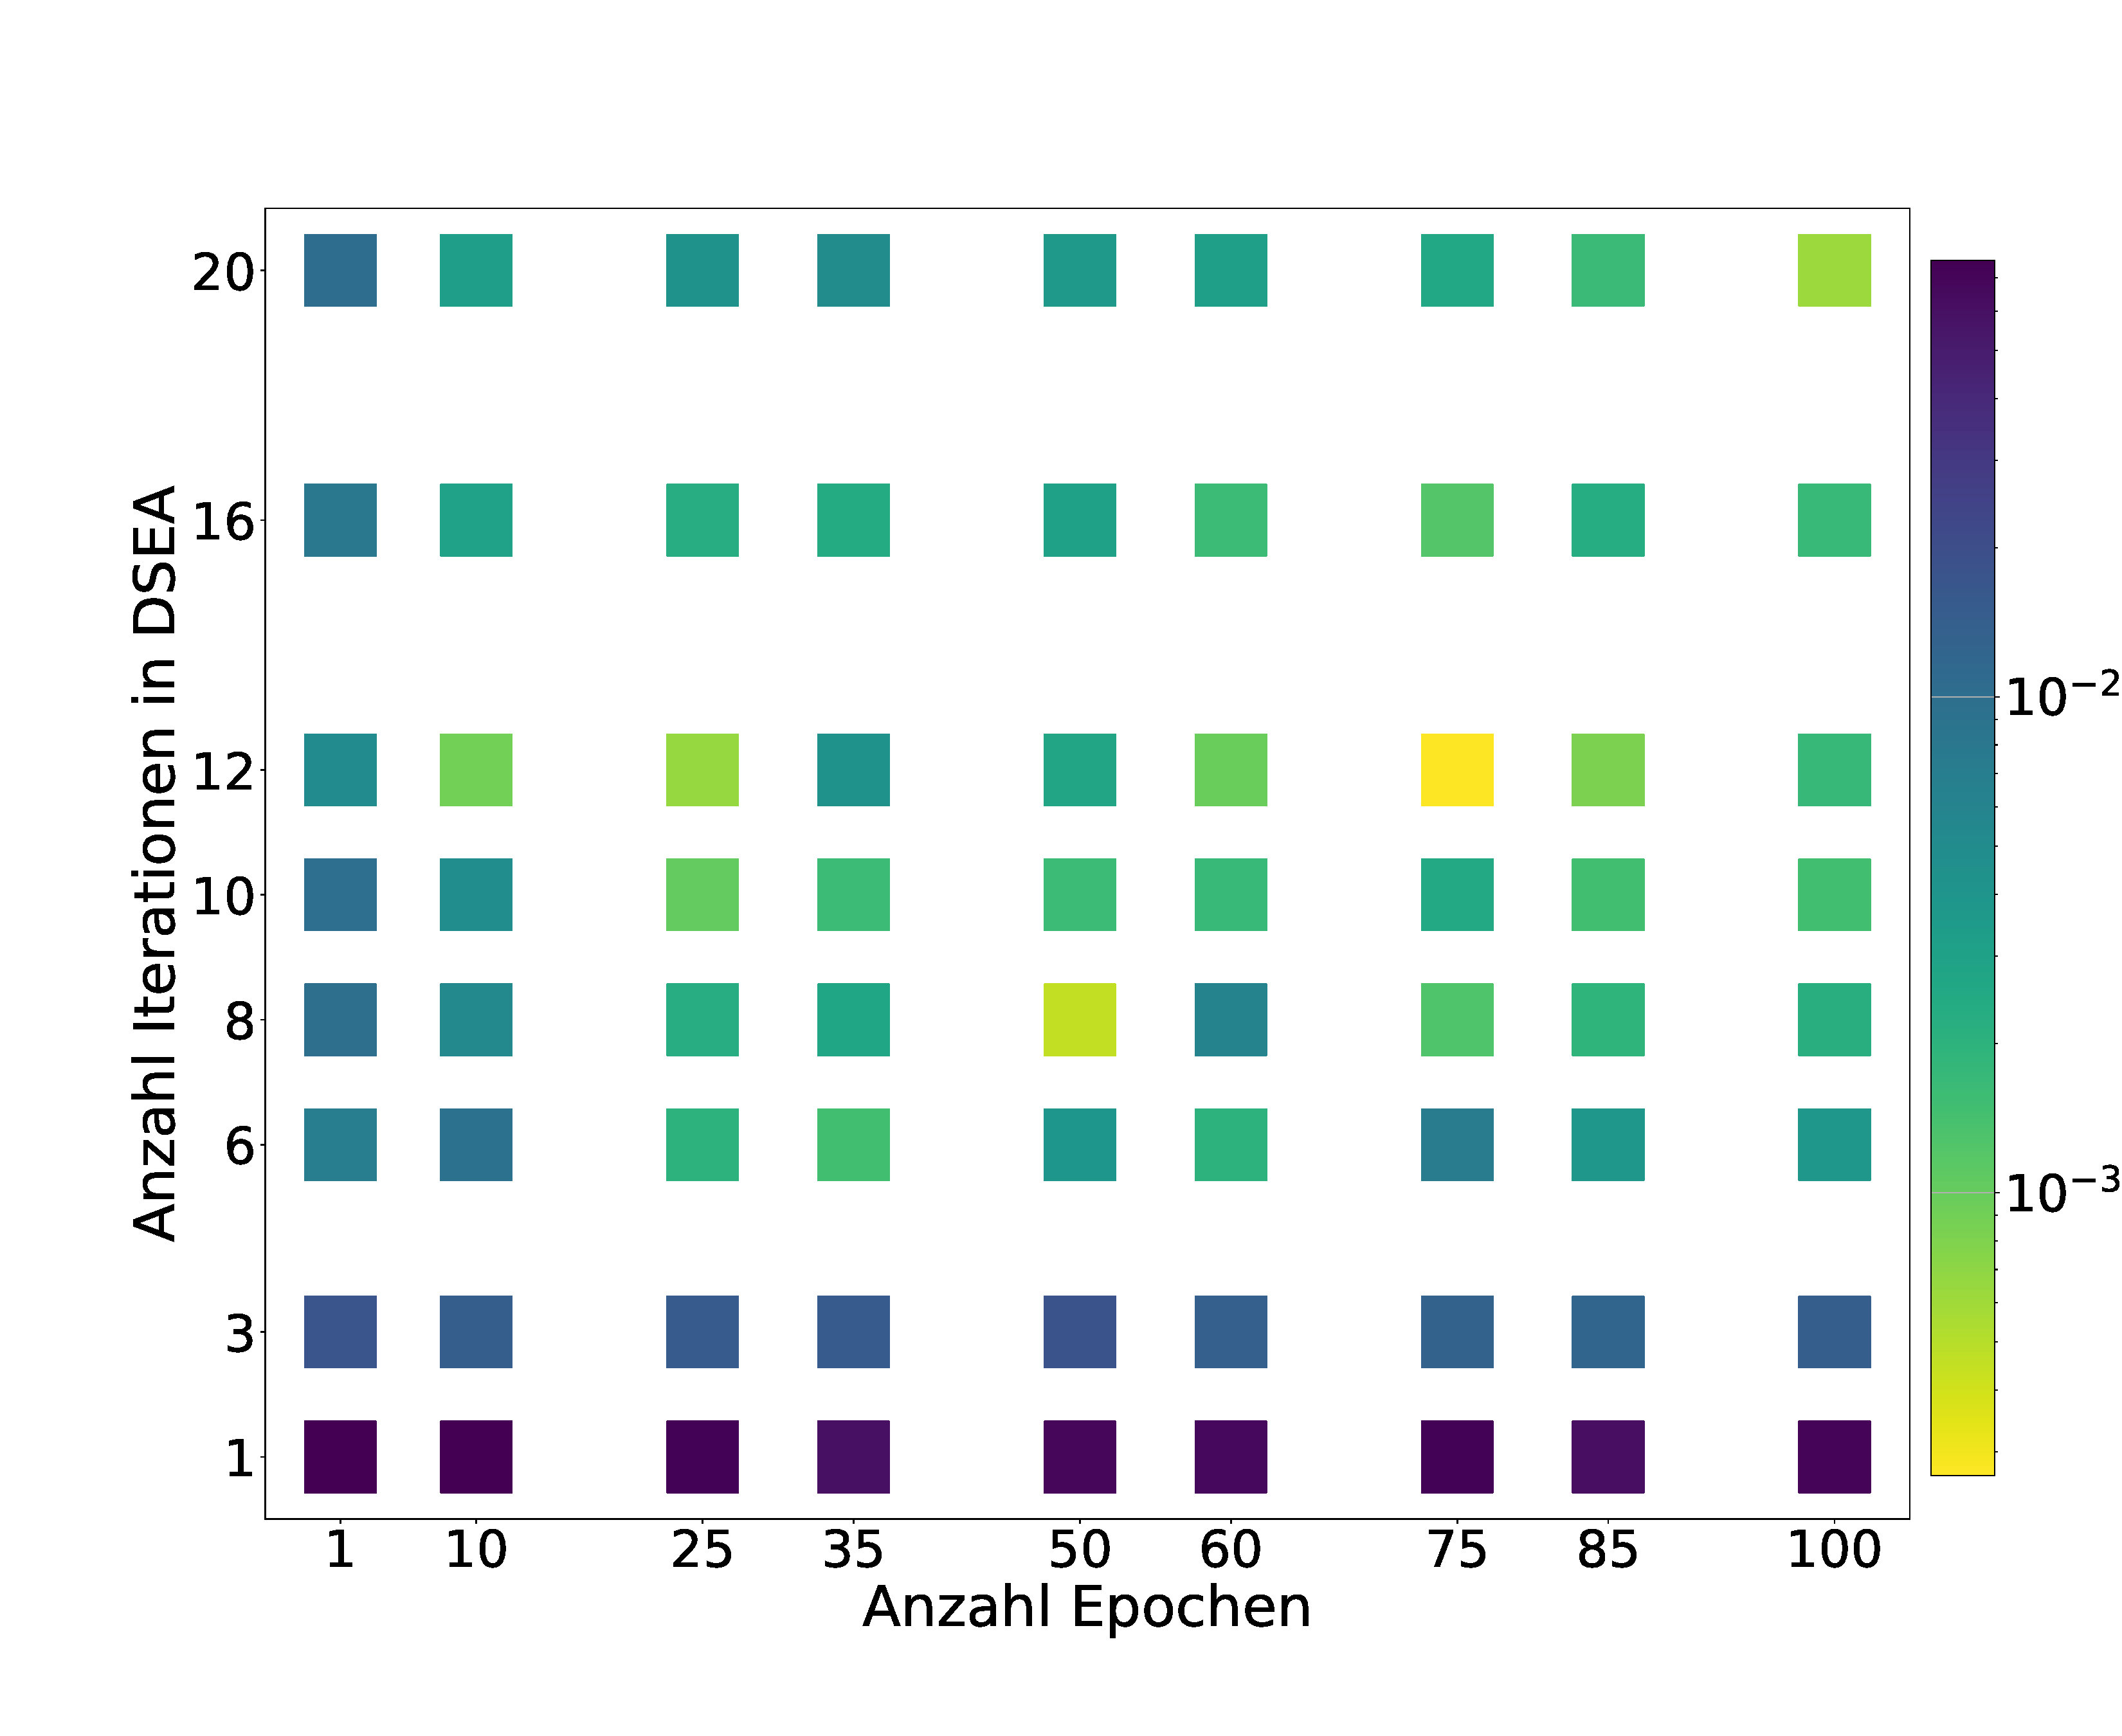
\includegraphics[width=1\textwidth]{Plots/DSEA/False/scatter_chi2.pdf}
    \caption[Ergebnisse der Gittersuche für mehrere (Anzahl: $n_\text{Iterationen}$) NN in DSEA]{Streudiagramm zur Darstellung der Ergebnisse der Gittersuche für Modell 1 (one\_model=False).
    In jeder DSEA-Iteration wird ein neues Modell erstellt und der Trainingsprozess beginnt von vorne.
    Die logarithmische Farbskala gibt den $\Chi^2$-Abstand zwischen dem wahren und vorhergesagten Spektrum an.
    }
    \label{fig:scatter_false}
\end{figure}

% trainings history: model 1 (one_model=False)
\begin{figure}%
    \begin{subfigure}{0.5\textwidth}%
        \centering%
        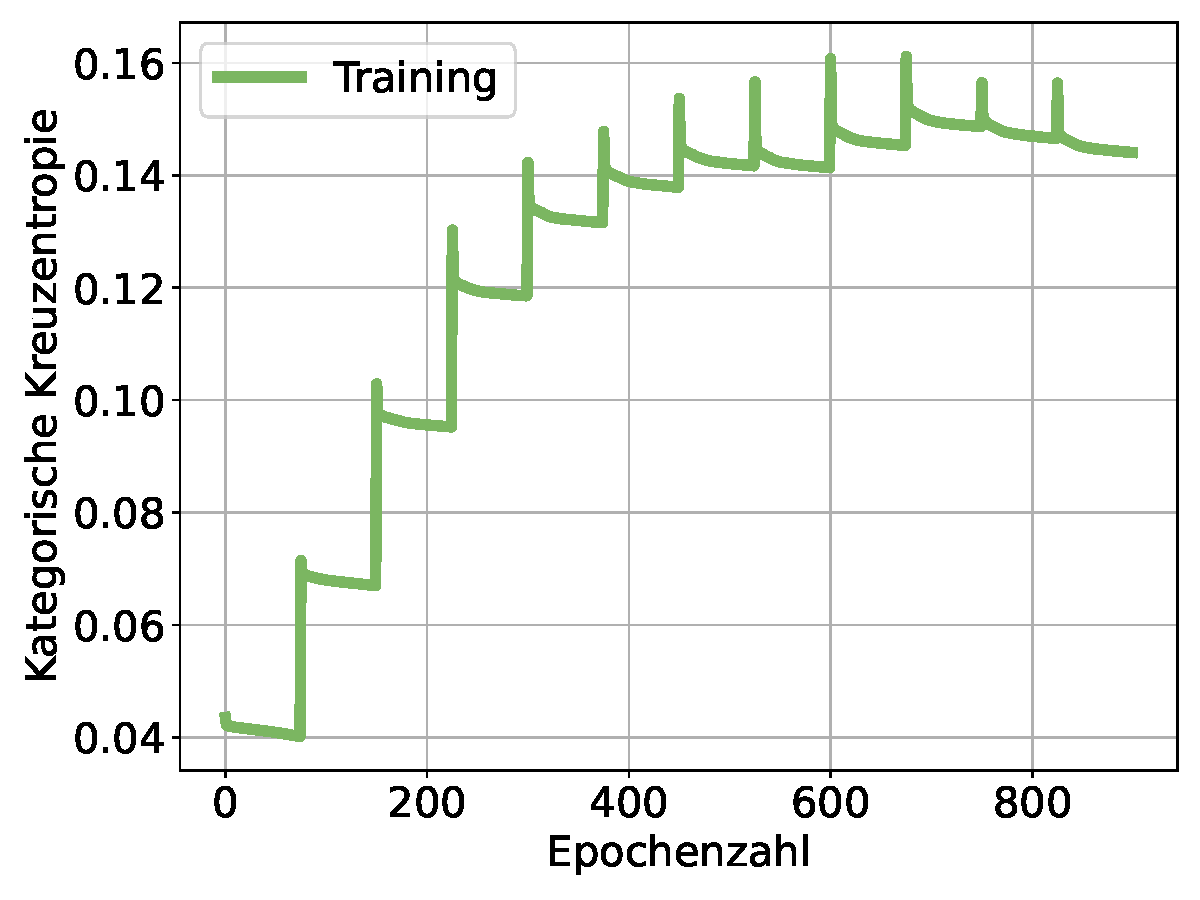
\includegraphics[height=5cm]{Plots/DSEA/False/loss.pdf}%
        \caption{Kostenfunktion: Kategorische Kreuzentropie}%
        %\label{fig:NN_loss}%
    \end{subfigure}%
    \hfill% Fills available space in the center -> space between figures
    \begin{subfigure}{0.5\textwidth}%
        \centering%
        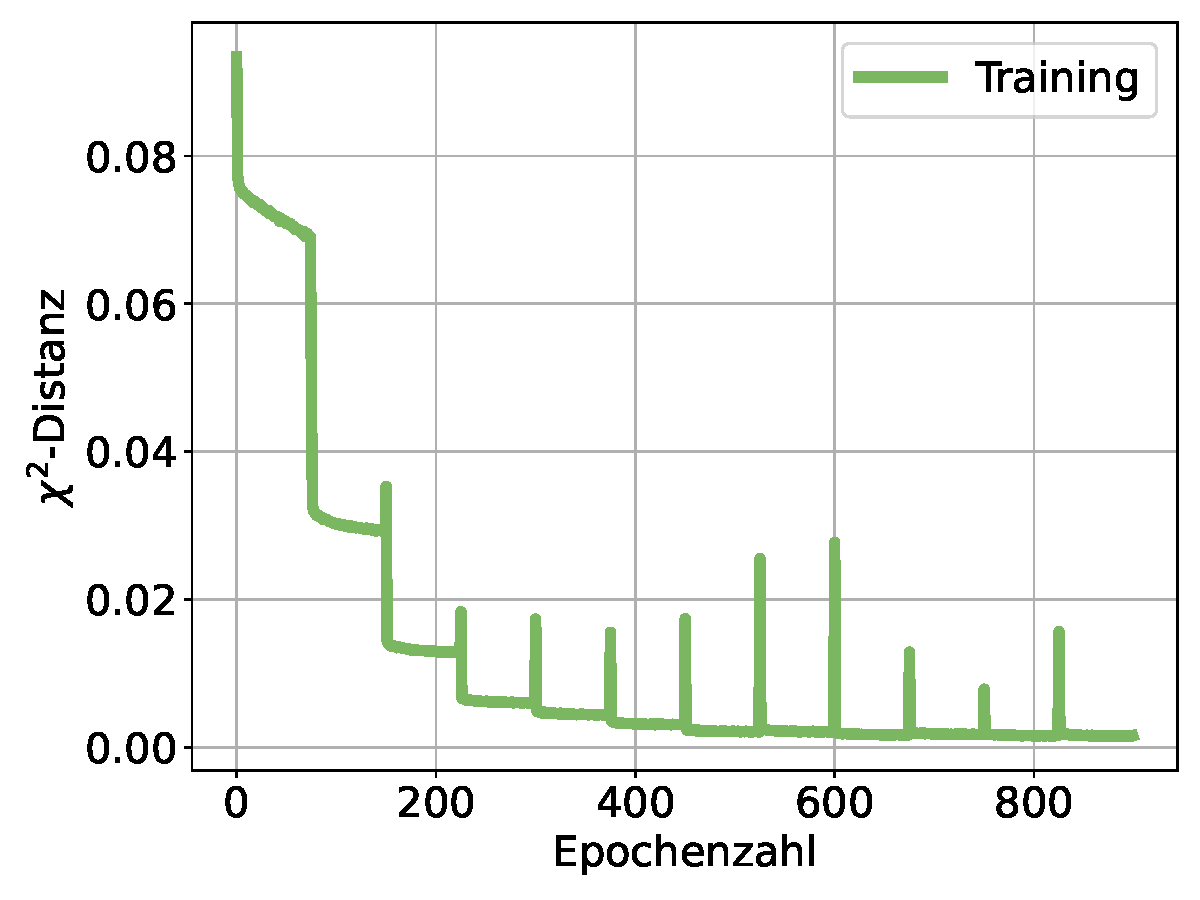
\includegraphics[height=5cm]{Plots/DSEA/False/chi.pdf}%
        \caption{Metrik: $\Chi^2$-Distanz}%
        %\label{fig:NN_chi}%
    \end{subfigure}%
    \caption[Verlauf des Trainingsprozesses des 1. Modells in DSEA]{Verlauf des Trainingsprozess des 1. Modells mit dem Parameter one\_model=False.
    In jeder DSEA-Iteration wird ein neues Modell mit aktualisierten Gewichten trainiert.
    Zum einen ist die Kostenfunktion \textit{kategorische Kreuzentropie} und zum anderen die \textit{Chi-Quadrat-Distanz} als Metrik in Abhängigkeit der Epochenzahl aufgeführt.
    }
    \label{fig:dsea_history_false}%
\end{figure}%}

% spectrum: model 1 (one_model=False)
\begin{figure}
    \centering
    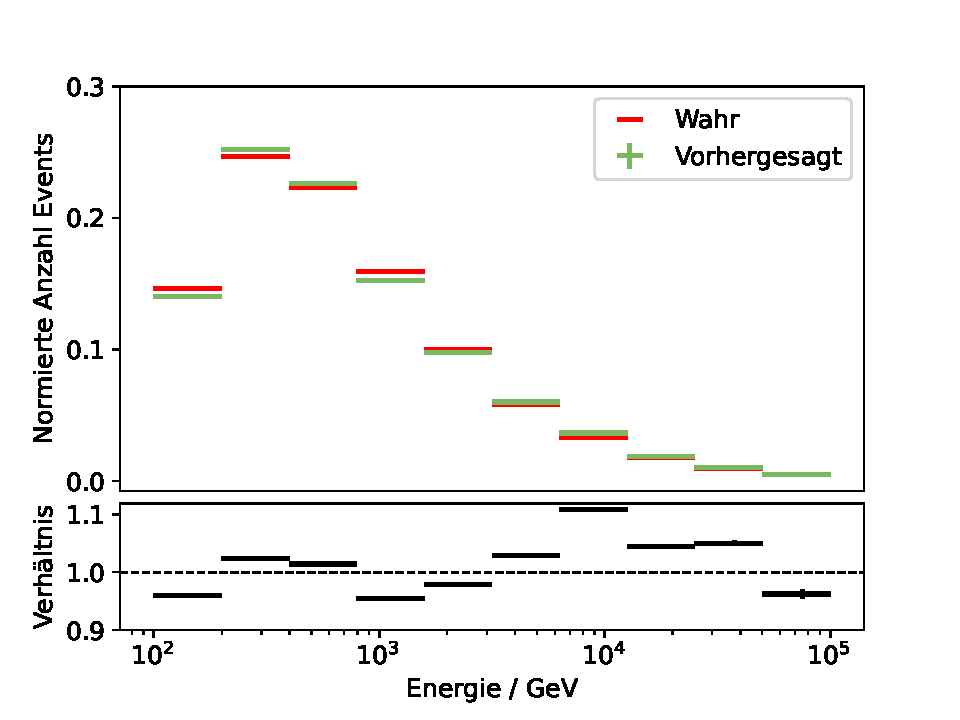
\includegraphics[width=0.9\textwidth]{Plots/DSEA/False/spectrum_dist_10bins_75ep_500000samples_200pulls.pdf}
    \caption[Spektrum des 1. Modells in DSEA]{Das entfaltete Spektrum des 1. Modells mit dem Parameter \textit{one\_model=False} und der zugehörige Verhältnis-Plot.
    In jeder DSEA-Iteration wird ein neues Modell mit aktualisierten Gewichten trainiert.
    }
    \label{fig:dsea_spectrum_false}
\end{figure}

% bootstrap: model 1 (one_model=False)
\begin{figure}%
    \centering%
    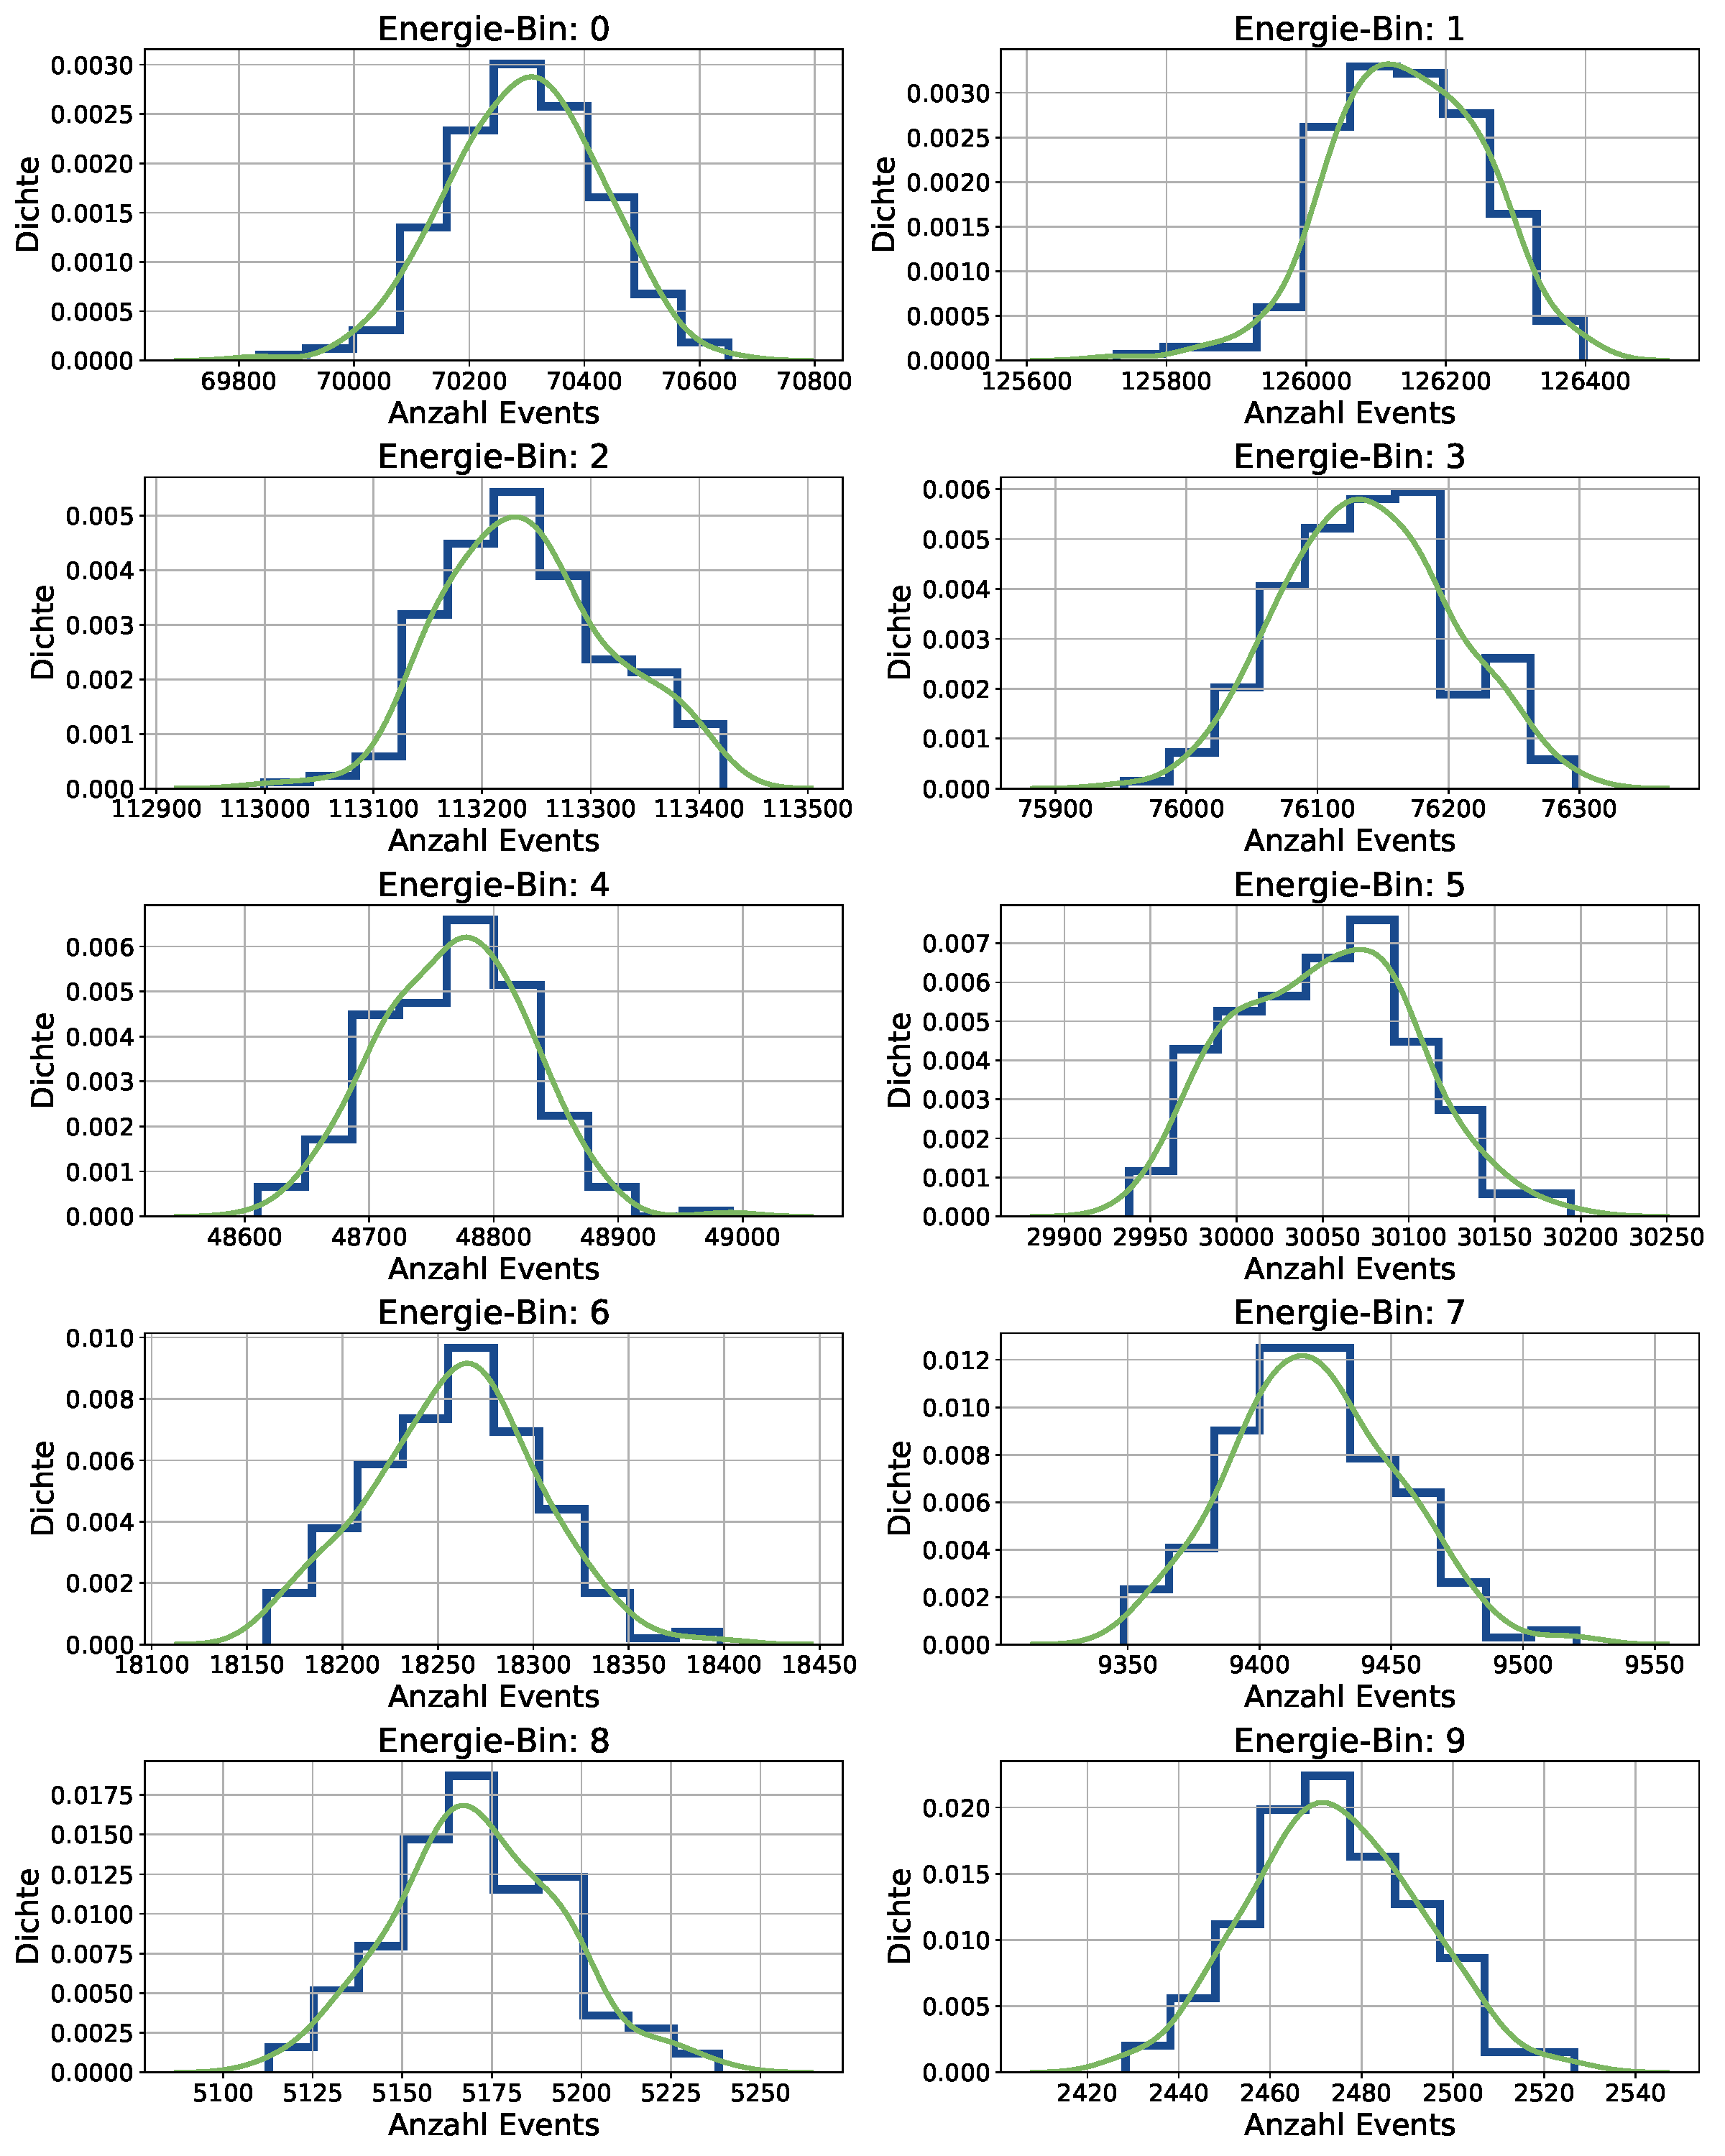
\includegraphics[width=\textwidth]{Plots/DSEA/False/class_dist_10bins_12it_75ep_500000samples_200pulls.pdf}%
    \caption[Ergebnisse des Bootstrapping-Vefahrens für das 1. Modell in DSEA]{Das blaue Histrogramm stellt die Verteilung der Bootstrap-Ergebnisse für Modell 1 (\textit{one\_model=False}) mit 200 Iterationen dar.
    Die rote Funktion repräsentiert einen Kerndichteschätzer(KDE) mit Gaußkern.
    Die Bin-Höhe wird durch den Median angegeben.
    Über das untere und obere Quantil werden die Unsicherheiten bestimmt.
    }%
    \label{fig:dsea_bootstrap_false}%
\end{figure}%

% bootstrap: model 2 (one_model=True)
\begin{figure}%
    \centering%
    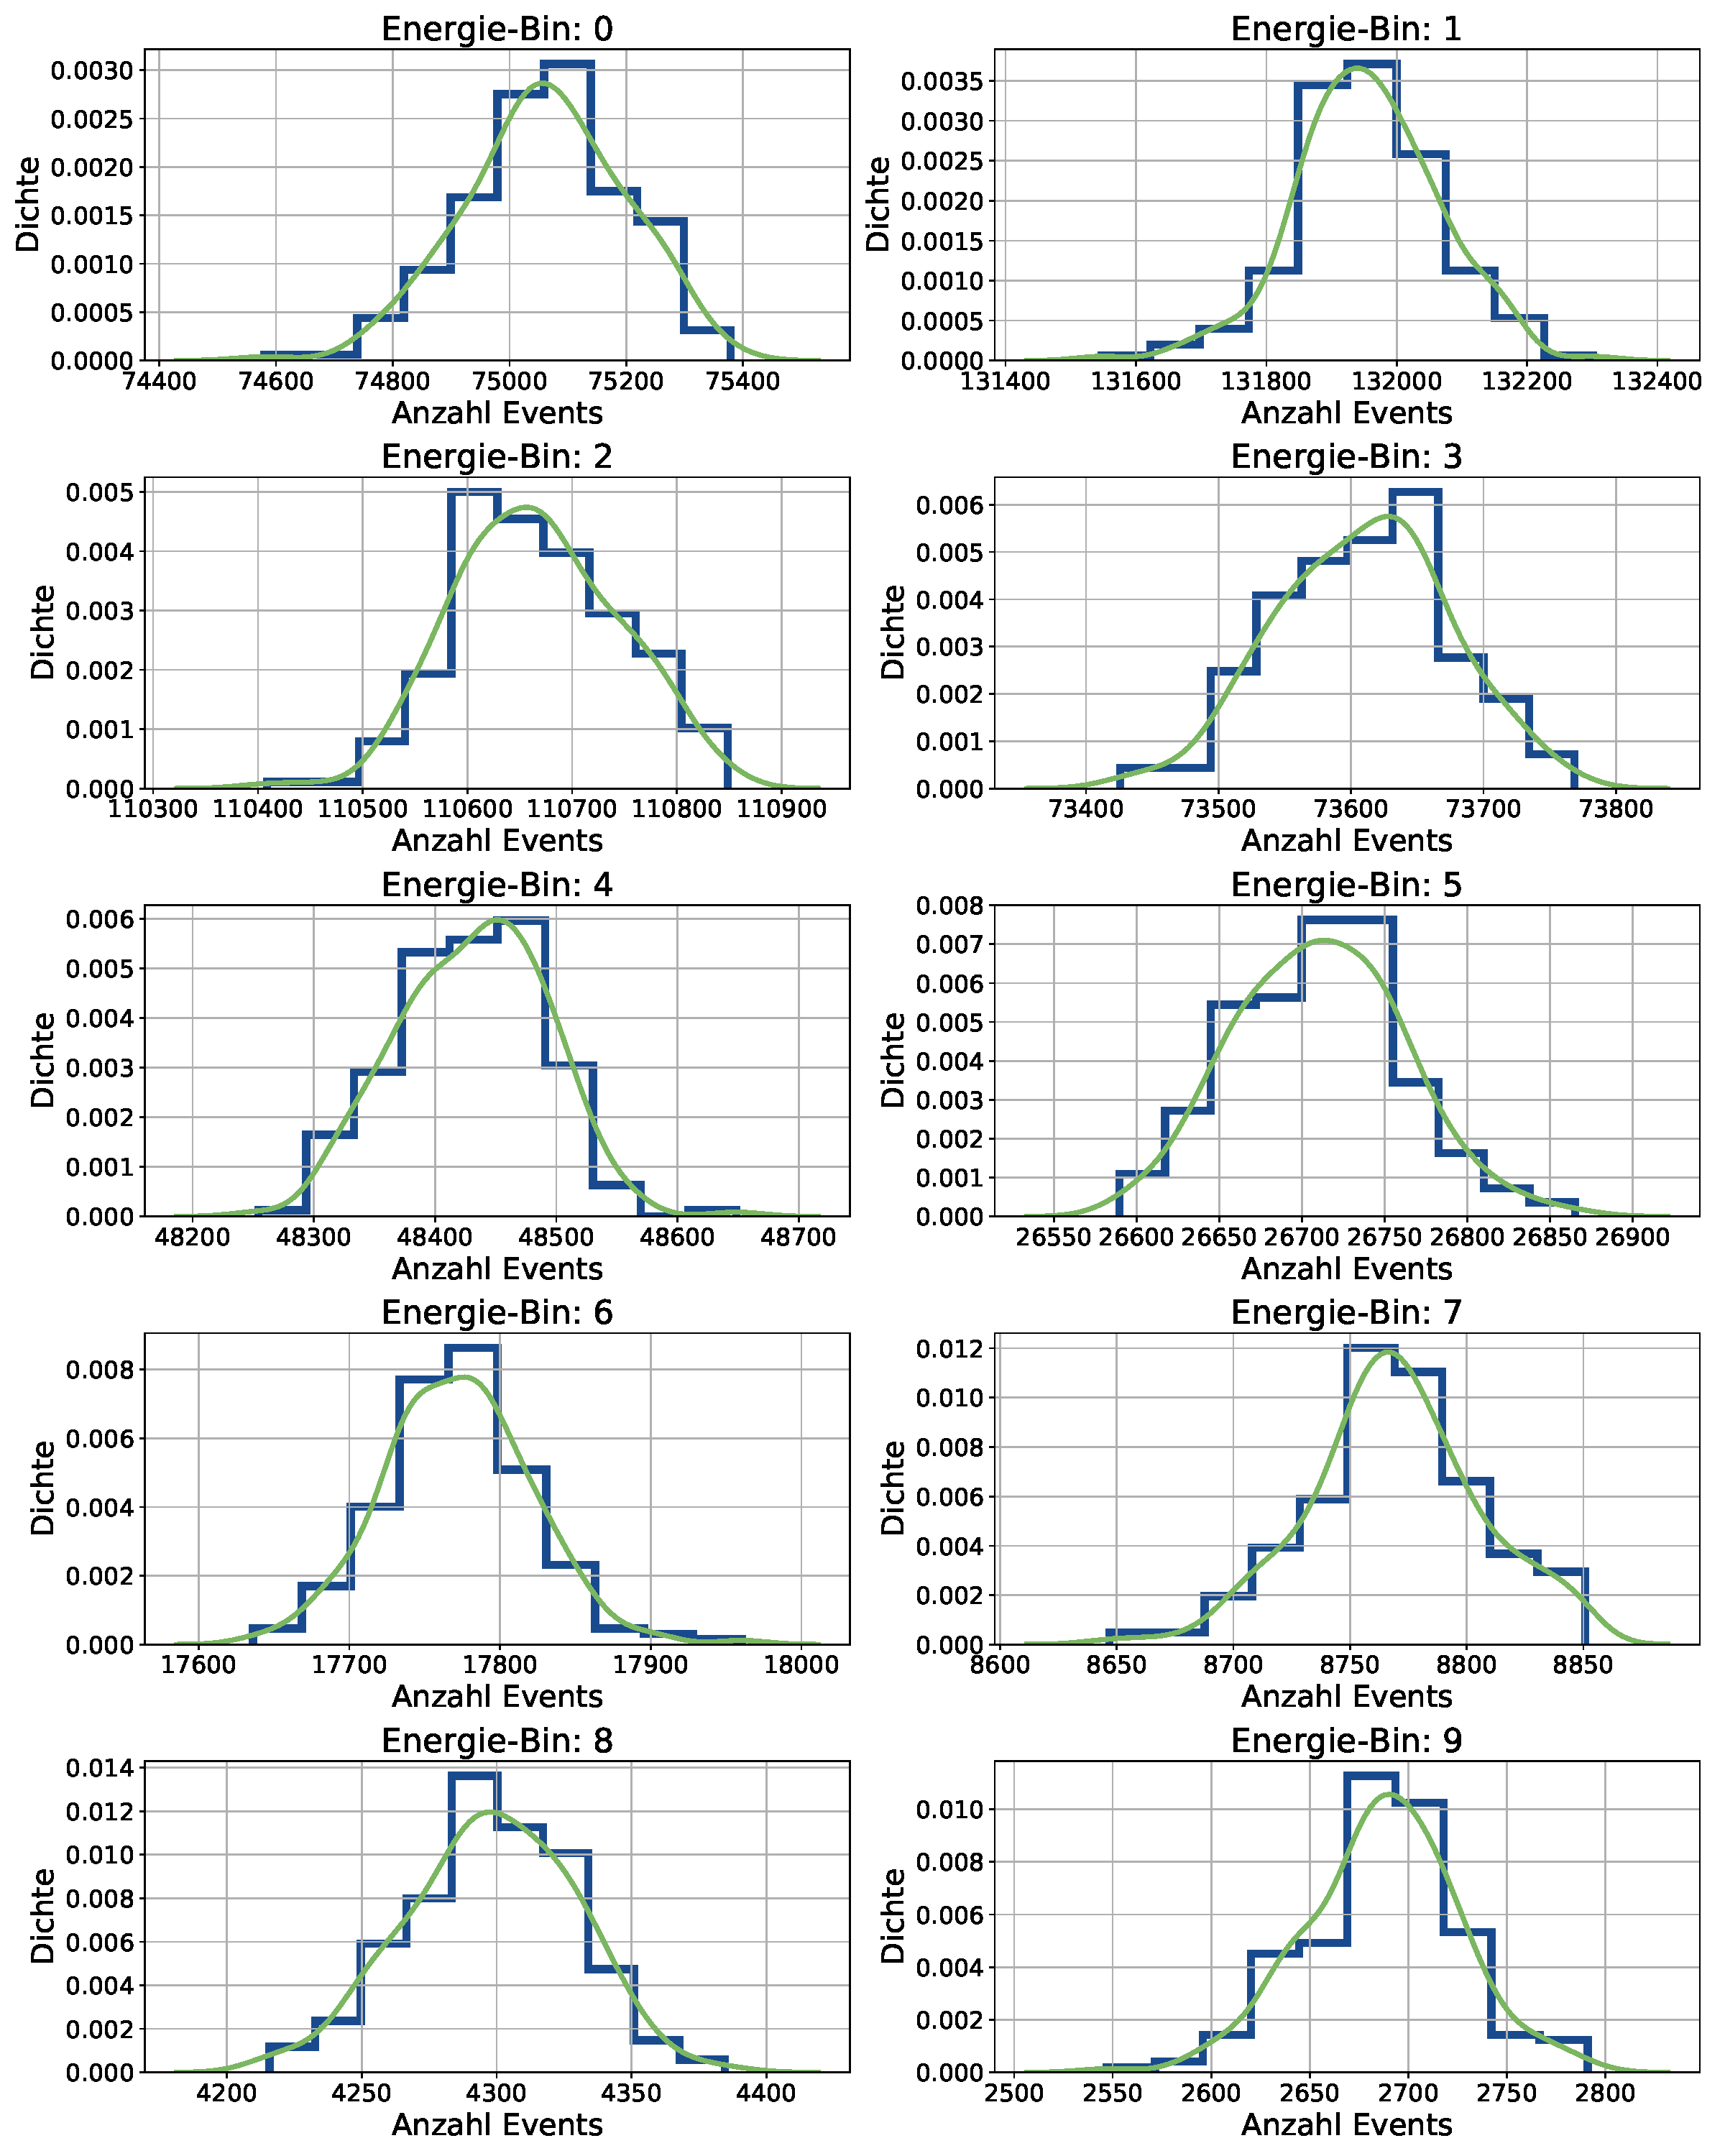
\includegraphics[width=\textwidth]{Plots/DSEA/True/class_dist_10bins_16it_60ep_500000samples_200pulls.pdf}%
    \caption[Ergebnisse des Bootstrapping-Vefahrens für das 2. Modell in DSEA]{Das blaue Histrogramm stellt die Verteilung der Bootstrap-Ergebnisse für Modell 2 (\textit{one\_model=True}) mit 200 Iterationen dar.
    Die rote Funktion repräsentiert einen Kerndichteschätzer(KDE) mit Gaußkern.
    Die Bin-Höhe wird durch den Median angegeben.
    Über das untere und obere Quantil werden die Unsicherheiten bestimmt.
    }%
    \label{fig:dsea_bootstrap_true}%
\end{figure}%

% single events: model 1(one_model=False)
\begin{figure}%
    \centering%
    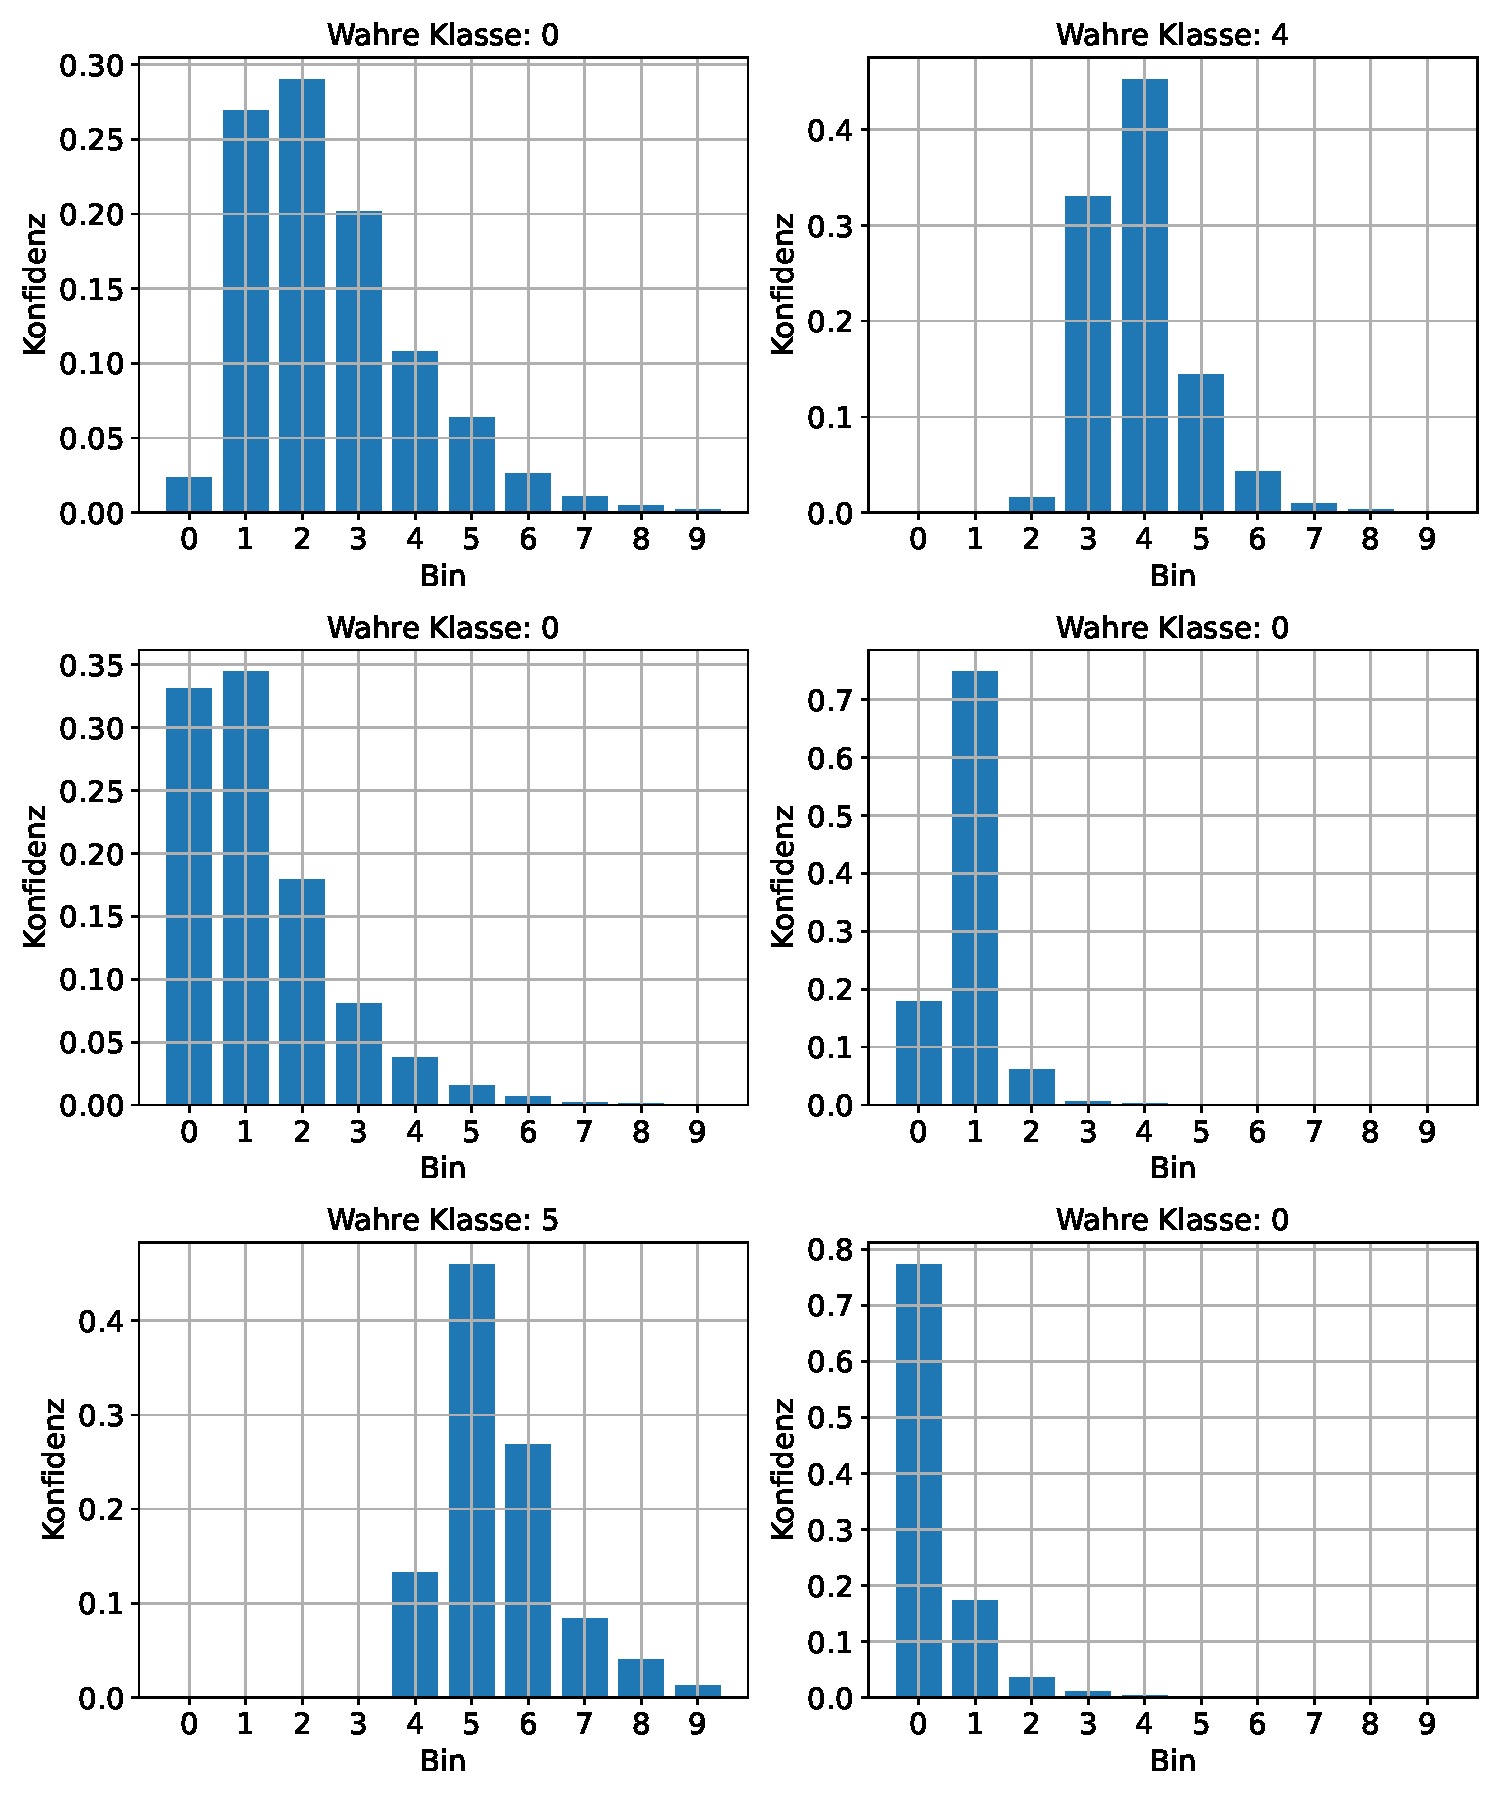
\includegraphics[width=\textwidth]{Plots/DSEA/False/SingleEvents_10bins_75ep_500000samples_200pulls.pdf}%
    \caption[Vorhersage einzelner Events des 1. Modells in DSEA]{Vorhersage einzelner Events des 1. Modells (\textit{one\_model=False}).
    Jedem Energie-Bin wird eine Konfidenz zugewiesen.
    Sie gibt die Zugehörigkeit des Events zu diesem Bin an.
    }%
    \label{fig:dsea_single_events_false}%
\end{figure}%

% single events: model 2(one_model=True)
\begin{figure}%
    \centering%
    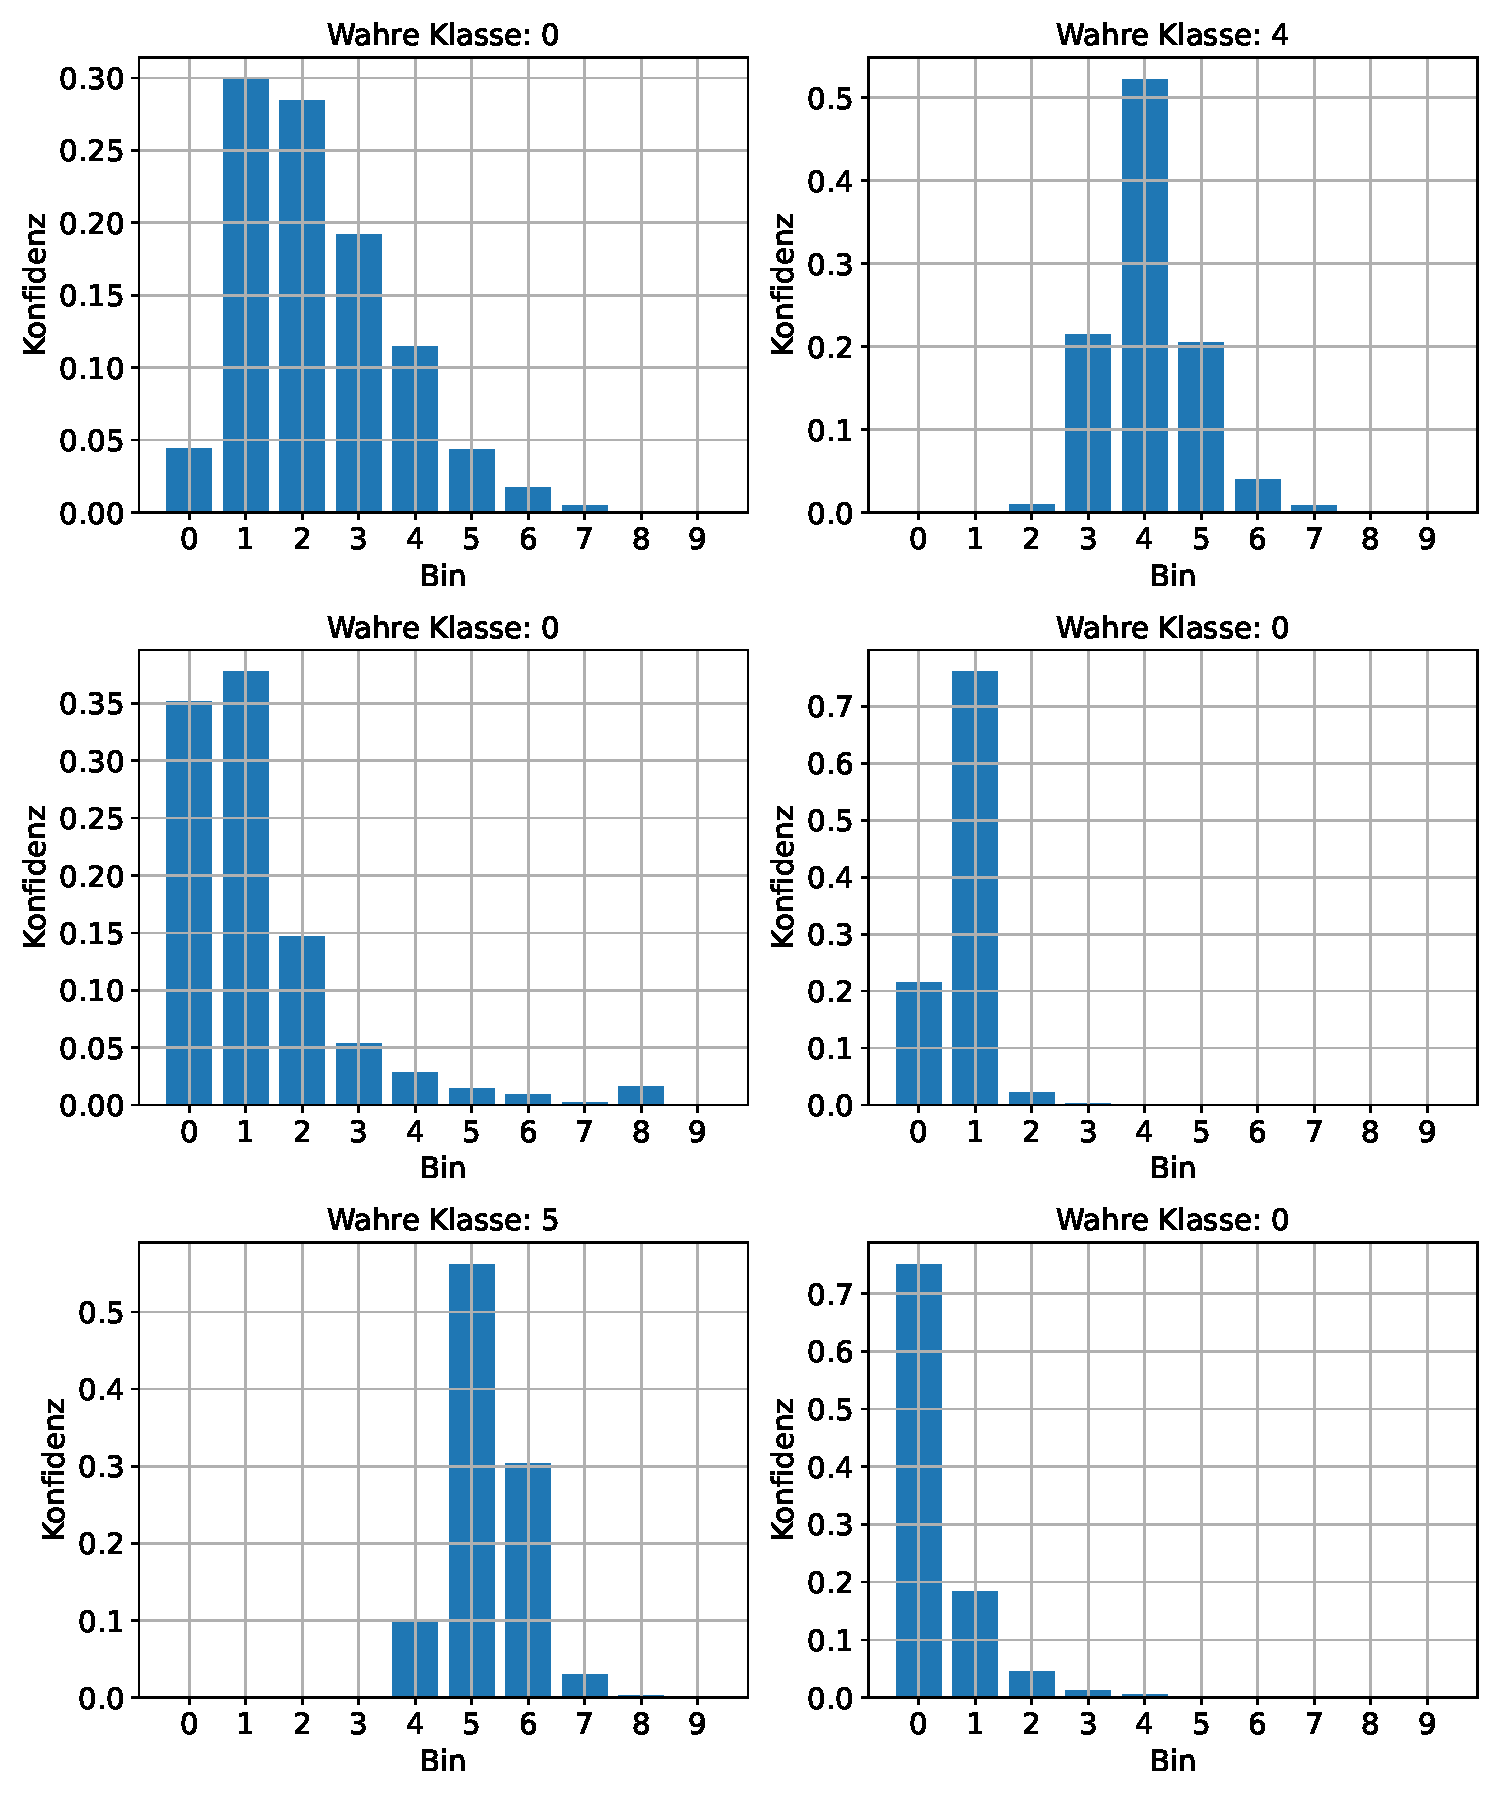
\includegraphics[width=\textwidth]{Plots/DSEA/True/SingleEvents_10bins_60ep_500000samples_200pulls.pdf}%
    \caption[Vorhersage einzelner Events des 2. Modells in DSEA]{Vorhersage einzelner Events des 2. Modells (\textit{one\_model=True}).
    Jedem Energie-Bin wird eine Konfidenz zugewiesen.
    Sie gibt die Zugehörigkeit des Events zu diesem Bin an.
    }%
    \label{fig:dsea_single_events_true}%
\end{figure}

% correlation matrix: model 1 (one_model=True)
\begin{figure}
    \centering
    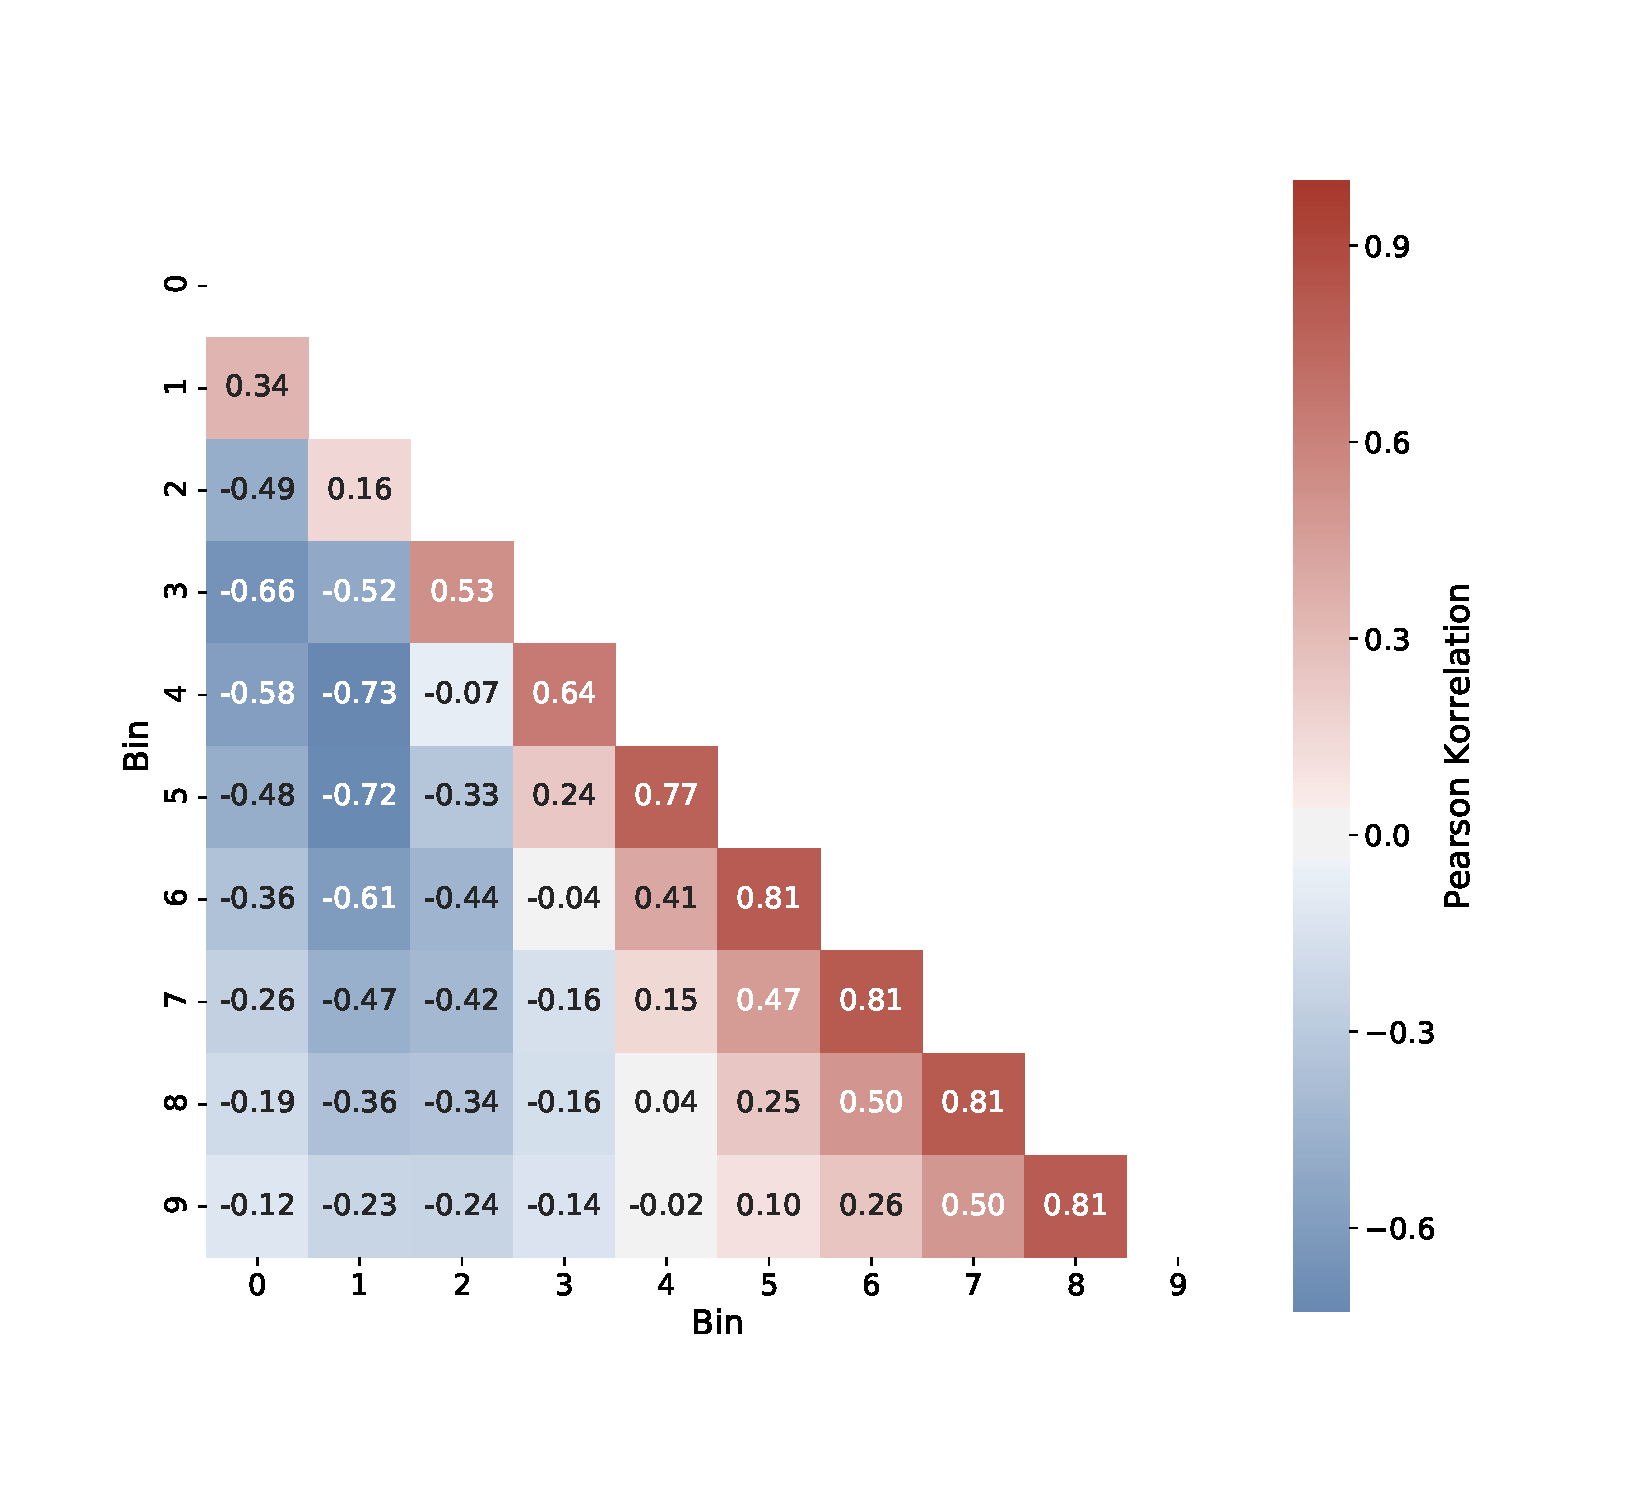
\includegraphics[width=1\textwidth]{Plots/DSEA/False/correlation_matrix.pdf}
    \caption[Korrelationsmatrix des 1. Modells in DSEA]{Die Korrelationsmatrix gibt die Korrelationen zwischen den entfalteten Energie-Bins an.
    Es handelt sich um das 1. Modell (\textit{one\_model=False}).
    }
    \label{fig:dsea_correlation_false}
\end{figure}
\chapter{Abhängigkeit der Entfaltung vom Trainingsspektrum}

\begin{figure}
    \centering
    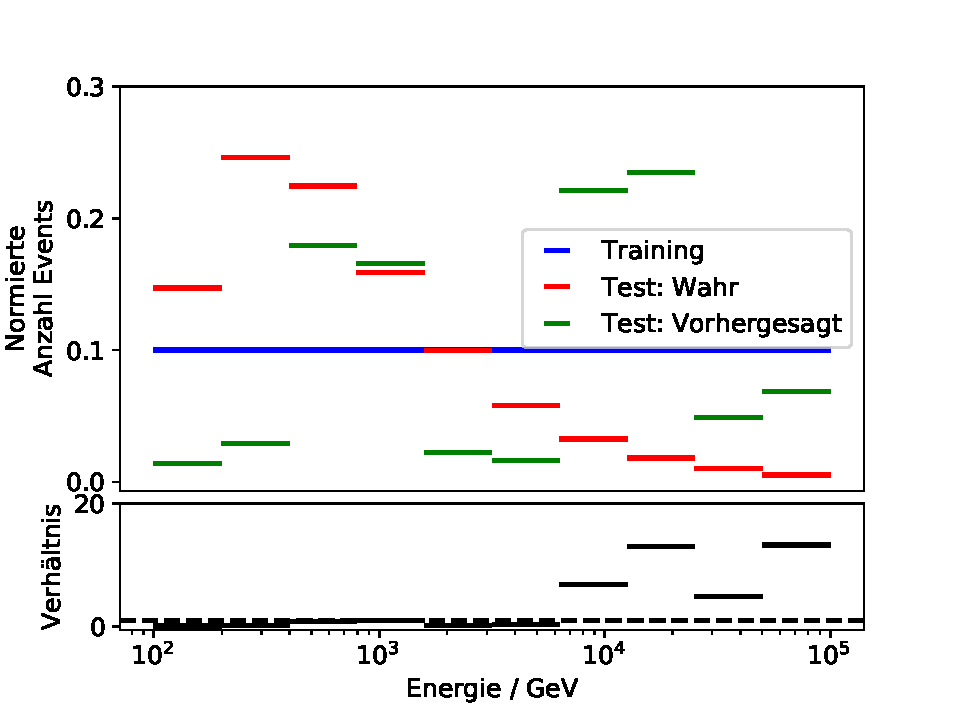
\includegraphics[width=0.9\textwidth]{Plots/BIAS/DSEA/spectrum_16it_60ep_True.pdf}
    \caption[Überprüfung des Bias: Spektrum des 2. Modells in DSEA]{Das mit einem NN in DSEA entfaltete Energiespektrum der Neutrinos.
    Das NN (Modell 2) wird in DSEA auf einem Datensatz mit gleichverteilten Klassen trainiert.
    Zum Vergleich der Spektren der Trainingsdaten (Blau), der wahren Evaluationsdaten (Rot) und der entfalteten Evaluationsdaten (Grün).
    }
    \label{fig:bias_dsea_true}
\end{figure}

\cleardoublepage
% \phantomsection

\listoffigures
\addcontentsline{toc}{chapter}{\listfigurename}
\backmatter
\printbibliography

\chapter{Danksagung}
Ich möchte mich bei dem gesamten Lehrstuhl bedanken, bei dem ich mich die letzten Monate sehr gut aufgehoben gefühlt habe.
Besonderen Dank gilt dabei Prof. Dr. Dr. Wolfgang Rhode und meinen direkten Ansprechpartnern Karolin Hymon, Leonora Kardum und Tim Ruhe, die mir bei jeglichen Fragen weitergeholfen haben.
\\
Die Diskussionen und Anregungen im wöchentlichen Meeting mit der DSEA-Gruppe haben die Arbeit erst ermöglicht.
Auch möchte ich Mirko Bunse für die Einbringung der technischen Seite danken.
\\
Mein Dank gilt ebenfalls Nicolai Weitkämper, der seine Bachelorarbeit parallel zu einem ähnlichen Thema geschrieben hat.
So konnten wir uns bei organisatorischen Dingen und technischen Problemen unterstützen und über inhaltliche Aspekte diskutieren.

\cleardoublepage
% From https://www.tu-dortmund.de/studierende/im-studium/pruefungsangelegenheiten/allgemeine-vordrucke/
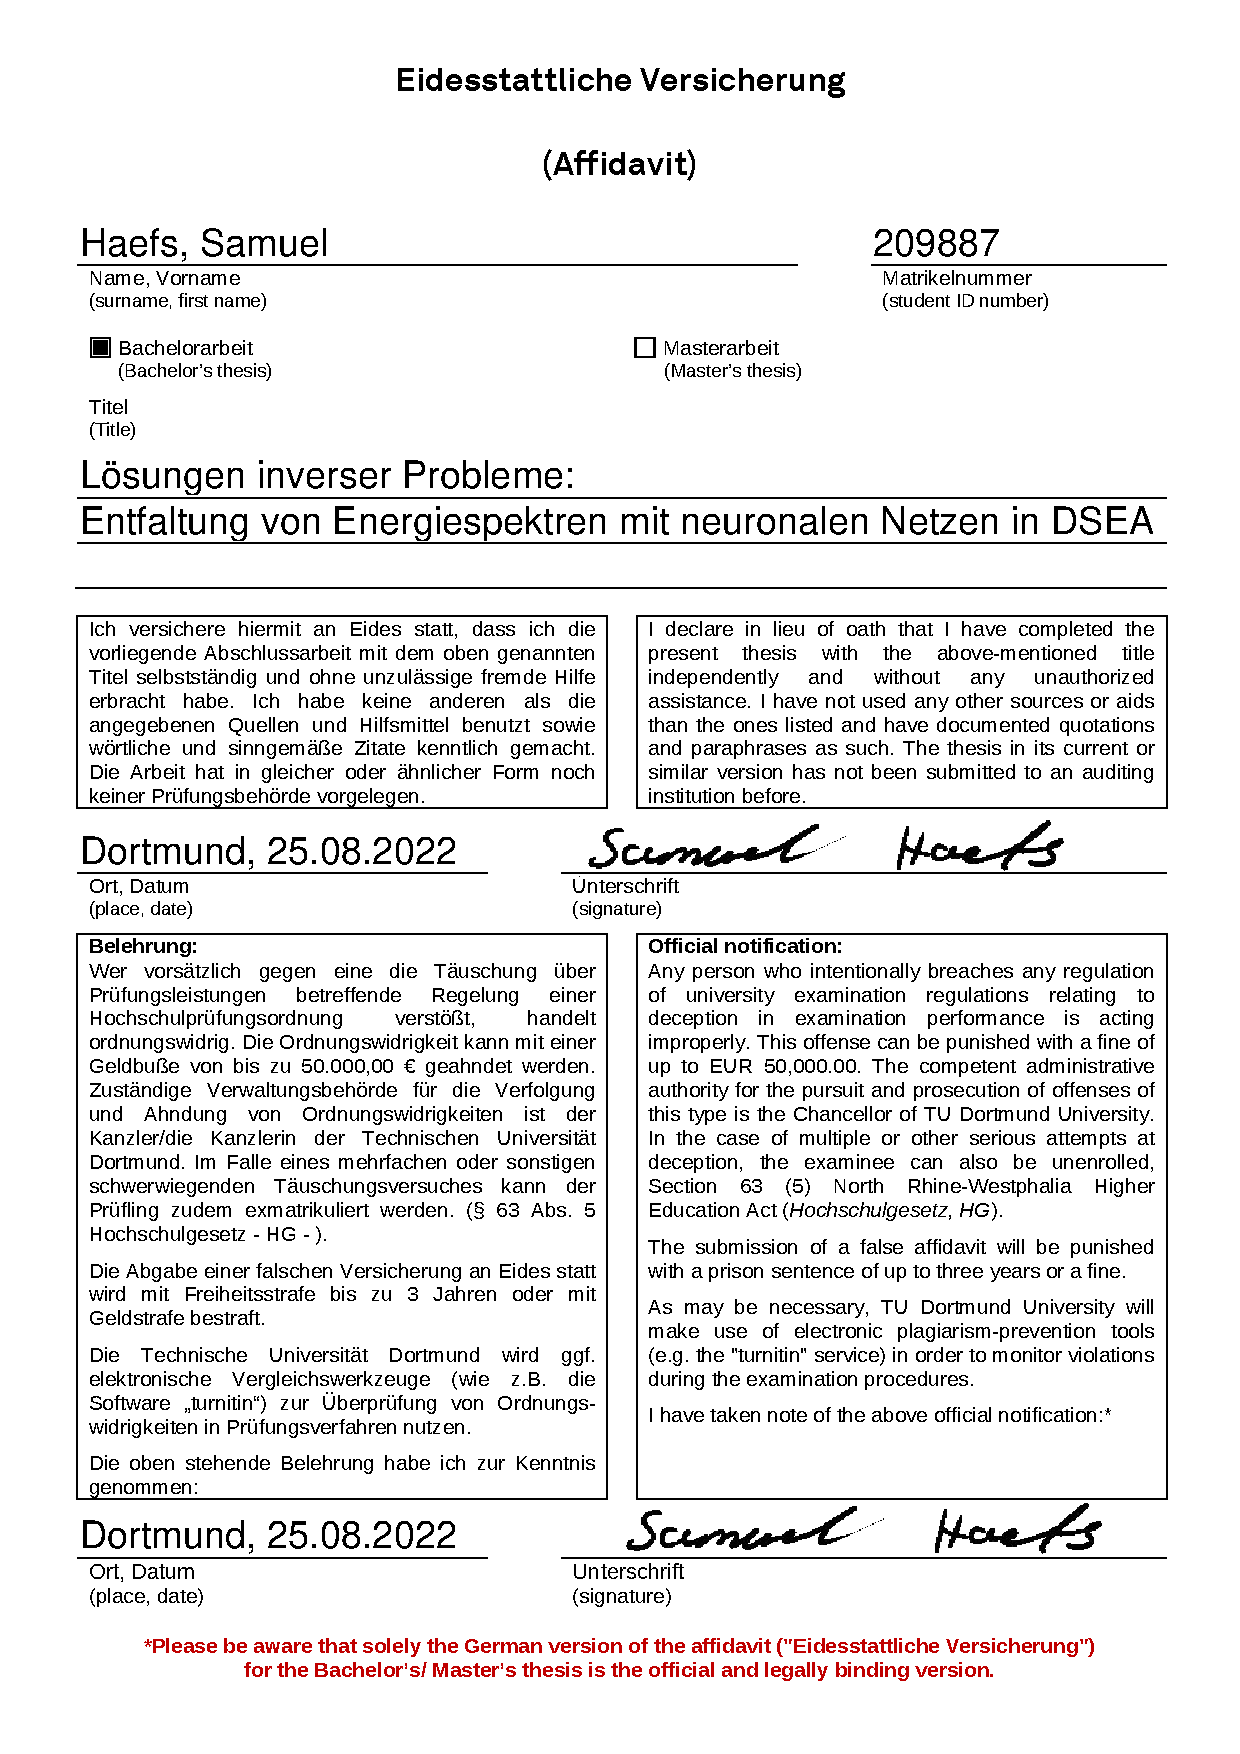
\includepdf{content/Eidesstattliche_Versicherung.pdf}

\end{document}
